%%%%%%%%%%%%%%%%%%%%%%%%%%%%%%%%%%%%%%%%%%%%%%%%%%%%%%%%%%%%%%%%%%%%%%%%%%%%%
%%%
%%% File: thesis.tex, version 1.9, May 2016
%%%
%%% =============================================
%%% This file contains a template that can be used with the package
%%% cs.sty and LaTeX2e to produce a thesis that meets the requirements
%%% of the Computer Science Department from the Technical University of Cluj-Napoca
%%%%%%%%%%%%%%%%%%%%%%%%%%%%%%%%%%%%%%%%%%%%%%%%%%%%%%%%%%%%%%%%%%%%%%%%%%%%%

\documentclass[12pt,a4paper,twoside]{report}         
\usepackage{cs}              
\usepackage{times}
\usepackage{graphicx}
\usepackage{latexsym}
\usepackage{amsmath,amsbsy}
\usepackage{amssymb}
\usepackage[matrix,arrow]{xy}
\usepackage[T1]{fontenc}
\usepackage{ae,aecompl}
\usepackage{romanian} %definitii pentru diacritice; 
\usepackage{amstext}
\usepackage{graphics}
\usepackage[T1]{fontenc}
\usepackage{ae,aecompl}
%\usepackage{algorithm}
%\usepackage{algorithmic}
\usepackage{color}
\usepackage{color}
\usepackage{listings}
\usepackage{verbatim}
\usepackage{subcaption}
\usepackage[final]{pdfpages}

\usepackage{algorithm2e}
\usepackage{tabularx}

% \mastersthesis
\diplomathesis
% \leftchapter
\centerchapter
% \rightchapter
\singlespace
% \oneandhalfspace
% \doublespace

\renewcommand{\thesisauthor}{Nicoleta COROCEA}    %% Your name.
\renewcommand{\thesismonth}{Iunie}     %% Your month of graduation.
\renewcommand{\thesisyear}{2019}      %% Your year of graduation.
\renewcommand{\thesistitle}{EXPLICAREA 'INV'A'T'ARII AUTOMATE FOLOSIND LIMBAJ NATURAL 'SI ONTOLOGII} % Title
\renewcommand{\thesissupervisor}{Conf.Dr.Eng. Adrian GROZA}
\newcommand{\department}{FACULTATEA DE AUTOMATIC'A 'SI CALCULATOARE\\
DEPARTAMENTUL CALCULATOARE}
\newcommand{\thesis}{LUCRARE DE LICEN'T'A}
\newcommand{\uline}[1]{\rule[0pt]{#1}{0.4pt}}
%\renewcommand{\thesisdedication}{P'arin'tilor mei}
\newcommand{\utcnlogo}{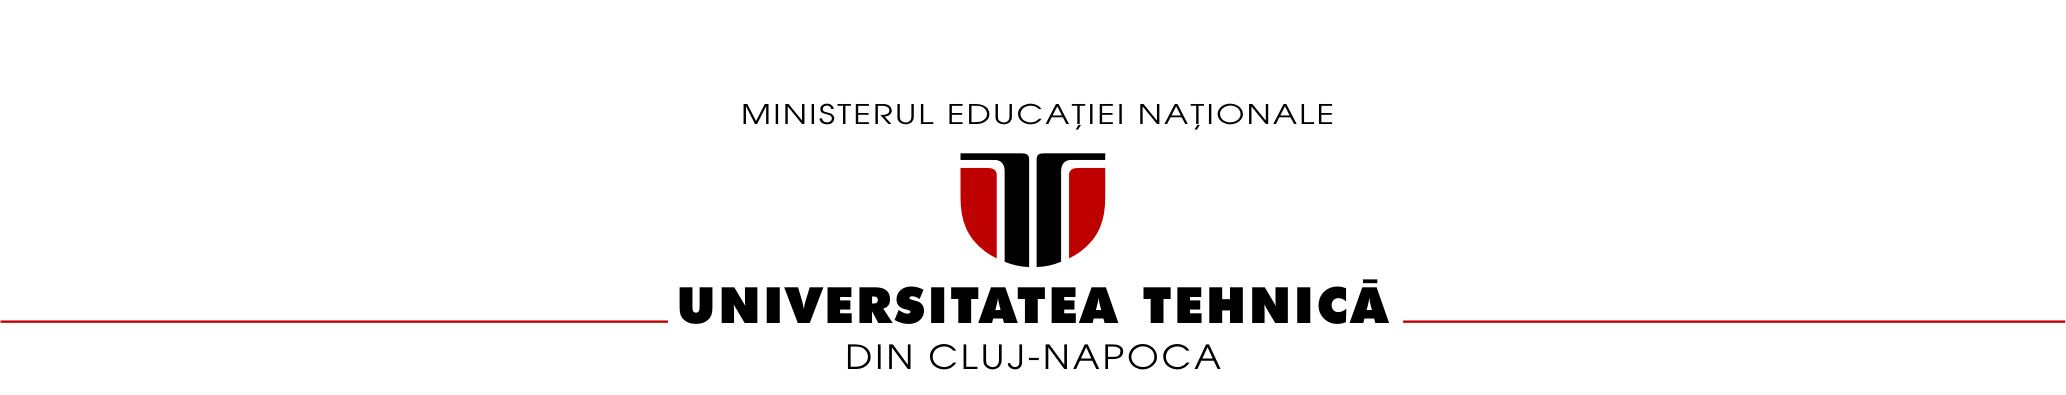
\includegraphics[width=15cm]{img/utcn.jpg}}
\newtheorem{example}{Exemplu}
\begin{document}

%\frontmatter
%\pagestyle{headings}

\newenvironment{definition}[1][Defini'tie.]{\begin{trivlist}
\item[\hskip \labelsep {\bfseries #1}]}{\end{trivlist}}



%\thesistitle                    %% Generate the title page.
%\authordeclarationpage                %% Generate the declaration page.


\begin{center}
%\includegraphics[width=15cm]{img/tucn.jpg}  
\utcnlogo

{\bf \department}

\vspace{4cm}

{\bf \thesistitle} %LICENSE THESIS TITLE}

\vspace{1.5cm}

\thesis

\vspace{6cm}

Absolvent: {\bf \thesisauthor} 

Conduc'ator 'stiin'tific: {\bf \thesissupervisor}

\vspace{3cm}
{\bf \thesisyear}
\end{center}

\thispagestyle{empty}
\newpage

\begin{center}
\utcnlogo

{\bf \department}
\end{center}
\vspace{0.5cm}

%\begin{small}
\begin{tabular}{p{7cm}p{8cm}}
 %\hspace{-1cm}& VIZAT,\\
 \hspace{-1cm}DECAN, & DIRECTOR DEPARTAMENT,\\
\hspace{-1cm}{\bf Prof. dr. ing. Liviu MICLEA} & {\bf Prof. dr. ing. Rodica POTOLEA}\\  
\end{tabular}
 
\vspace{2cm}

\begin{center}
Absolvent: {\bf \thesisauthor}

\vspace{1cm}

{\bf \thesistitle}
\end{center}

\vspace{1cm}

\begin{enumerate}
 \item {\bf Enun'tul temei:} {\it Scurt'a descriere a temei lucr'arii de licen't'a 'si datele ini'tiale}
\item {\bf Con'tinutul lucr'arii:} {\it (enumerarea p'ar'tilor componente) Exemplu: Pagina de prezentare, aprecierile coordonatorului de lucrare, titlul capitolului 1, titlul capitolului 2, titlul capitolului n, bibliografie, anexe.}
\item {\bf Locul document'arii:} {\it Exemplu}: Universitatea Tehnic'a din Cluj-Napoca, Departamentul Calculatoare
\item {\bf Consultan'ti:}
\item {\bf Data emiterii temei:} 1 Noiembrie 2018
\item {\bf Data pred'arii:} 8 iulie 2019 {\it (se va completa data pred'arii)}
  \end{enumerate}
\vspace{1.2cm}

\hspace{6cm} Absolvent: \uline{6cm} 

\vspace{0.5cm}
\hspace{6cm} Coordonator 'stiin'tific: \uline{5cm} 
%\end{small}

\thispagestyle{empty}

\newpage

\begin{center}
\utcnlogo

{\bf \department}
\end{center}

\vspace{0.5cm}

\begin{center}
{\bf
Declara'tie pe proprie r'aspundere privind\\ 
autenticitatea lucr'arii de licen't'a}
\end{center}
\vspace{1cm}



Subsemnatul(a) \\
\uline{14.8cm}, 
legitimat('a) cu \uline{4cm} seria \uline{3cm} nr. \uline{4cm}\\
CNP \uline{9cm}, autorul lucr'arii \uline{2.8cm}\\
\uline{16cm}\\
\uline{16cm}\\
elaborat'a 'in vederea sus'tinerii examenului de finalizare a studiilor de licen't'a la Facultatea de Automatic'a 'si Calculatoare, Specializarea \uline{7cm} din cadrul Universit'a'tii Tehnice din Cluj-Napoca, sesiunea \uline{4cm} a anului universitar \uline{3cm}, declar pe proprie r'aspundere, c'a aceast'a lucrare este rezultatul propriei activit'a'ti intelectuale, pe baza cercet'arilor mele 'si pe baza informa'tiilor ob'tinute din surse care au fost citate, 'in textul lucr'arii 'si 'in bibliografie.

Declar, c'a aceast'a lucrare nu con'tine por'tiuni plagiate, iar sursele bibliografice au fost folosite cu respectarea legisla'tiei rom\ia ne 'si a conven'tiilor interna'tionale privind drepturile de autor.

Declar, de asemenea, c'a aceast'a lucrare nu a mai fost prezentat'a 'in fa'ta unei alte comisii de examen de licen't'a.

'In cazul constat'arii ulterioare a unor declara'tii false, voi suporta sanc'tiunile administrative, respectiv, \emph{anularea examenului de licen't'a}.

\vspace{1.5cm}

Data \hspace{8cm} Nume, Prenume

\vspace{0.5cm}

\uline{3cm} \hspace{5cm} \uline{5cm}

\vspace{1cm}
\hspace{9.4cm}Semn'atura

\thispagestyle{empty}

\newpage

%\clearpage 
%\newpage

%\begin{comment}
{\color{red}{\bf De citit 'inainte} (aceast'a pagin'a se va elimina din versiunea final'a)}:
\begin{enumerate}
 \item Cele trei pagini anterioare (foaie de cap'at, foaie sumar, declara'tie) se vor lista pe foi separate (nu fa't'a-verso), fiind incluse 'in lucrarea listat'a. 
 Foaia de sumar (a doua) necesit'a semn'atura absolventului, respectiv a coordonatorului.
 Pe declara'tie se trece data c\ia nd se pred'a lucrarea la secretarii de comisie.
 \item Pe foaia de cap'at, se va trece corect titulatura cadrului didactic 'indrum'ator, 'in englez'a (consulta'ti pagina de unde a'ti desc'arcat acest document pentru lista cadrelor didactice cu titulaturile lor).
 \item Documentul curent {\bf nu} a fost creat 'in MS Office. E posibil sa fie mici diferen'te de formatare. 
\item Cuprinsul 'incepe pe pagina nou'a, impar'a (dac'a se face listare fa't'a-verso), prima pagin'a din capitolul Introducere tot a'sa, fiind numerotat'a cu 1. % Pentru actualizarea cuprinsului, click dreapta pe cuprins (zona cuprinsului va apare cu gri), Update field-$>$Update entire table.
\item Vizualiza'ti (recomandabil 'si 'in timpul edit'arii) acest document % după ce activaţi vizualizarea simbolurilor ascunse de formatare (apăsaţi simbolul  din Home/Paragraph).
\item Fiecare capitol 'incepe pe pagin'a nou'a. % datorită simbolului ascuns Section Break (Next Page) care este deja introdus la capitolul precedent. Dacă ştergeţi din greşeală simbolul, se reintroduce (Page Layout -> Breaks).
\item Folosi'ti stilurile predefinite (Headings, Figure, Table, Normal, etc.)
\item Marginile la pagini nu se modific'a.
\item Respecta'ti restul instruc'tiunilor din fiecare capitol.
\end{enumerate}
\thispagestyle{empty} 
%\end{comment}

\pagenumbering{roman}
\setcounter{page}{1}

\newpage

\tableofcontents

\newpage

%\listoftables
%\listoffigures

\pagenumbering{arabic}
\setcounter{page}{1}

%%%%%%%%%%%%%%%%%%%%%%%%%%%%%%%%%%%%%%%%%%%%%%%%%%%%%%%%%%%%%%%%%%%%%%%
\chapter{Introducere - Contextul proiectului}

\pagestyle{headings}

 Interac'tiunile cu agen'tii inteligen'ti sunt privite cu ne'incredere datorit'a structurii de cutie neagr'a. Nevoia de a crea sisteme explicabile pentru a diminua scepticismul are 'si influen'te legale. 'In acest sens, Uniunea European'a sus'tine dreptul de a nu fi supus exclusiv unei decizii luate 'in totalitate de un algoritm. 'In capitolul curent se va descrie 'in prima parte cererea pentru explicabilitate pentru algoritmii de 'inv'a'tare. A doua parte abordeaz'a o conturare a solu'tiei problemei, c'at 'si impactul pe care 'il are asupra acesteia.
 
\section{Descrierea problemei}

C'autarea cuvintelor cheie $"machine\ learning"$ 'in cadrul motorului de c'autare Google a crescut de patru ori 'in ultimii 5 ani, ajun\ia nd la noi valori maxime 'in anul 2019, potrivit statisticilor\footnote{https://trends.google.com/trends/}. Amplificarea interesului pentru aria 'inv'a't'arii automate 'si dezvoltarea acestui domeniu este 'incurajat'a de cre'sterea num'arului de date disponibile folosite pentru antrenarea algoritmilor, aproxim\ia ndu-se c'a p\ia n'a 'in 2020, universul digital va atinge 44 de zettabytes. Mai mult de at\ia t, oamenii sunt interesa'ti, dar 'si sceptici cu privire la rezultatele pe care le poate da un algoritm. Acest fapt a condus la $Explainable AI$ (XAI), pentru explicarea procesului prin care un algoritm de 'inv'a'tare automat'a sau orice sistem inteligent ob'tine r'aspunsul.

Scopul XAI este de a oferi r'aspuns utilizatorului la 'intreb'arile care apar pentru sistemele de tipul cutie neagr'a, cum ar fi 'inv'a'tarea automat'a: "De ce ai f'acut asta? De ce nu ai f'acut altceva? C\ia nd reu'se'sti? C\ia nd e'suezi? C\ia nd e'suezi? C\ia nd pot avea 'incredere 'in tine? Cum corectez o eroare?". Aceste 'intreb'ari se afl'a 'in concordant'a cu urm'atorul citat ~\cite{monroe2018ai} din CACM (tradus): {\it "Este timpul ca inteligen'ta artificial'a s'a dep'a'seasc'a perioada de adolescen't'a, de joc, 'si s'a ia 'in serios no'tiunile de calitate 'si fiabilitate."}.

'In acela'si sens, politica Uniunii Europene 'in ceea ce prive'ste prodec'tia datelor pledeaz'a pentru dreptul la explica'tie. Prin urmare, nu este surprinz'ator faptul c'a articolul 22 din GDPR include "Dreptul de a nu fi supus unei decizii bazate exclusiv pe prelucrarea automat'a". Tot pe acest plan, inclusiv Facebook explic'a utilizatorilor de ce fac parte din grupul 'tint'a al reclamelor pe care le v'ad. 

Domeniul 'stiin'tei datelor responsive~\cite{van2017responsible} este un prim exemplu de aria ce poate beneficia pe urm XAI. Opinia noastr'a este ca numai 'inv'at'area automat'a 'in sine nu este suficient'a pentru a lua o decizie. Chiar 'si cu clasificare foarte exact'a, este nevoie de un fel de garan'tie sau ra'tionament penntrua lua decizii.

Multe abord'ari ale explicabilit'a'tii sunt disponibile din ultimii ani, cum ar fi cercetarea lui Toni et al. pentru argumentare 'si explicare~\cite{ANNWithXAI}. 'In mod similar, Gilpin et al.~\cite{Gilpin2019ExplainingLearning} se concentreaz'a asupra metodelor explicabile 'in arhitecturile neurale ad\ia nci, oferind o imagine de anslamblu a interpretabilit'a'tii 'inv'a't'arii automate. Aceste realiz'ari nu se opresc la explicarea 'inv'a't'arii automate, ci se extind 'si spre alte domenii, cum ar fi medicina, biologia 'si limbajul natural. 
'In domeniul biomedical, Holzinger et al. \cite{Holzinger2018FromAI} sus'tin implementarea 'inv'a't'ari automate interactive, {\it iML}. Aceast'a abordare pune omul 'in bucla algoritmului, combin\ia nd cuno'stin'tele umane cu seturi de date biomedicale incomplete, pentru a ob'tine ceea ce nici un om, nici un computer nu ar putea sa fac'a singur. 'In acest sens, este de 'in'teles necesitatea pentru XAI, explicarea deciziilor sistemelor inteligente. 

'In paralel cu aceste aspecte, odat'a cu tehnologia evolueaz'a 'intreaga popula'tie. Oamenii au devenit din ce 'in ce mai atra'si de tehnologie, iar internetul le ofer'a o multitudine de surse de informare, cum ar fi motoarele de c'autare, forumuri 'si platforme de 'inv'a'tare online. Platforme precum  Coursera\footnote{https://www.coursera.org/} sau Udemy\footnote{https://www.udemy.com/} furnizeaz'a informa'tii care pot fi accesate 'in orice moment, fiind prezentate 'in mod pl'acut 'si 'incuraj\ia nd utilizatorii s'a se 'imbun'at'a'teasc'a. 'In acest domeniu, sistemele de tip $Question\ Answering$ precum Stack Overflow\footnote{https://stackoverflow.com/} au ca scop complementarea platformelor de 'inv'a'tare online, prin extragerea de informa'tii structurate pe baza 'intreb'arilor.

\section{Conturarea solu'tiei}
'In domeniul  exist'a diferite abord'ari ale sistemelelor care r'aspund la 'intreb'ari, c\ia t 'si a agen'tilor conversa'tionali. Din perspectiva popularit'a'tii, agen'tii conversa'tionali sunt mult mai populari datorit'a simul'arii conversa'tiei mai aproopiate de cea a oamenilor. Mai mult, ace'stia pot 'indeplini sarcini precum rezerv'ari sau apeluri telefonice. Asisten'ti virtuali precum Cortana 'si Google Assistant sus'tin activit'a'tile utilizatorilor 'in fiecare zi. Ace'stia dau r'aspunsuri scurte 'si nu neap'arat complexe, din domenii variate. Pe de alt'a parte, sistemele de tip $Question Answering$, precum Mind the Book (cu 'intreb'ari despre c'ar'ti) au un avantaj pe planul r'aspunsurilor mai detaliate, concentrate pe un anumit domeniu.

'In lucrarea de fa't'a se dezvolt'a un sistem de tip $Question Answering$ pentru no'tiuni de 'inv'a'tare automat'a care permite utilizatorilor s'a adreseze 'intreb'ari 'in limbaj natural pentru a ob'tine r'aspunsuri. Sistemul este unul explicativ-educativ, oferind transparen't'a 'in ceea ce prive'ste procedeul de extragere al r'aspunsului. Utilizatorilor le este permis s'a vizualizeze elementele ontologiei, s'a introduc'a intreb'ari 'in limbaj natural, s'a editeze interogarea aferent'a 'si sa ob'tin'a r'aspunsul prin dou'a metode. Arhitectura proiectului este dezvoltat'a pe nivele. Framework-ul Quepy este utilizat penntru a asigura translatarea din limbaj natural 'in limbaj de interogare SPARQL. Pentru extragerea r'aspunsului din ontologia OWL se utilizeaz'a ra'tionatorul Pellet 'si libr'aria pentru lucru cu structuri RDF, RDFLib. Interfa'ta utilizator este realizat'a 'in Angular, 'si un modul Spring Boot pune la dispozi'tie puncte terminale pentru utilizarea aplica'tiei.

'In continuare, capitolul~\ref{sec:objectives} cuprinde o descriere detaliat'a a obiectivelor 'si a pozi'tion'arii  sistemului. Studiul bibliografic al domenului problemei este cuprins de capitolul~\ref{sec:bibliographic_research}. Capitolul~\ref{ch:analysis} con'tine o ampl'a descriere a analizei 'si fundament'arii teoretice , urm\ia nd ca 'in capitlul~\ref{sec:proiectare} s'a se descrie arhitectura sistemului 'si implementarea acestuia, solu'tii alternative ale arhitecturii 'si scenarii de utilizare. Capitolul~\ref{sec:testing} 'inglobeaz'a testarea 'si validarea sistemului, capitolul~\ref{sec:instalare} cuprinde instruc'tiuni pentru instalarea sistemului 'si utilizarea acestuia. Capitolul~\ref{sec:concluzii} concluzioneaz'a lucrarea.



%%%%%%%%%%%%%%%%%%%%%%%%%%%%%%%%%%%%%%%%%%%%%%%%%%%%%%%%%%%%%%%%%%%%%%%%%
\chapter{Obiectivele Proiectului}
\label{sec:objectives}

'In acest capitol se vor descrie obiectivele sistemului dezvoltat, c\ia t 'si pozi'tionarea solu'tiei alese. De asemenea, sunt prezentate 'si descrise pe scurt 'si cerin'tele sistemului.

\section{Contextul sistemului}

Num'arul de informa'tii din cadrul internetului a crescut, acestea fiind nestructurate 'si contradictorii 'in multe cazuri. Acest fenomen este 'int\ia lnit 'si 'intr-un domeniu restr\ia ns ca {\it 'inv\ia 'tarea automat'a}. Mai mult de at\ia t, interac'tiunile cu un agen'tii inteligen'ti sunt privite cu scepticism 'si ne'incredere datorit'a r'aspunsurilor provenite dintr-o logic'a 'incapsulat'a 'intr-o cutie neagr'a. Ne'increderea 'in inteligen'ta artificial'a 'si necunoa'sterea principiilor de baz'a ale 'inv'at'arii automate determin'a oamenii s'a utilizeze sistemele 'invechite 'in detrimentul solu'tiilor noi, inteligente. Ace'stia continu'a s'a 'indeplineasc'a sarcini repetitive care ar putea fi u'surate utiliz'and 'inv'a'tarea automat'a. Tototdat'a, lipsa explica'tiilor poate avea un impact asupra legalit'a'tii deciziilor luate. Lipsa explica'tiilor 'si lipsa implic'arii utilizatorului 'in procesul de luare a deciziilor care 'il privesc 'indeaproape este un drept 'inc'alcat. Datorit'a acestor fapte, progresul sistemelor inteligente este 'incetinit. 
'In tabelul ~\ref{tab:pb_table} se prezint'a o descriere a problemei, al'aturi de solu'tii posibile ale acesteia.

\begin{table}
    \centering
    \begin{tabular}{p{3.5cm}|p{8.5cm}}
Problema &  Ne'increderea 'si scepticismul cu privire la solu'tiile inteligente datorate necunoa'sterii domeniului 'si al func'tion'arii 'inv'a't'arii automate. \\[1ex]
    \hline
afecteaz'a & Utilizatorii, dezvoltatorii de aplica'tii 'in domeniul 'inv'a't'arii automate.\\[1ex]
    \hline
efectele sunt & Supunerea la decizii luate 'in totalitate de un agent inteligent, c\ia t 'si sc'aderea utiliz'arii 'si dezvolt'arii solu'tiilor bazate pe inteligen'ta artificial'a.\\[1ex]
    \hline
o solu'tie de succes  ar trebui s'a fie& Capabil'a s'a r'aspund'a 'intreb'arilor 'in limbaj natural 'si s'a ofere transparen't'a 'in modul de ob'tinere a r'aspunsului.\\[1ex]
    \end{tabular}
     \caption{Declara'tia problemei}
    \label{tab:pb_table}
\end{table}

Politica Uniunii Europene privind protec'tia datelor oblig'a la acordarea explica'tiilor 'in cazul r'aspunsurilor date de agen'tii inteligen'ti. 'In articolul 22 din GDPR se sus'tine "Dreptul de a nu fi supus unei decizii bazate exclusiv pe prelucrarea automat'a". Astfel Uniunea European'a identific'a o surs'a a ne'increderii ca fiind lipsa explica'tiilor in contextul deciziilor bazate pe 'inv'a'tare automat'a, c\ia t 'si problema supunerii la deciziile luate de un agent inteligent. Sistemul dezvoltat dore'ste s'a rezolve problema ne'increderii 'si sa reduc'a scepticismul 'in utilizarea solu'tiilor inteligente existente. Acesta este bazat pe un agent explicativ al 'inv'a't'arii automate, care este disponibil prin intermediul unei interfe'te. Proiectul creat pune la dispozi'tie comunit'a'tii dezvoltatorilor de sisteme inteligente o solu'tie prin care pot s'a 'imp'art'a'seasc'a func'tionarea sistemelor automate, separat de mediul influen'tabil al diverselor pagini web. Sistemul explicativ va fi disponibil online 'si to'ti utilizatorii vor putea avea acces. 'In tabelul ~\ref{tab:solution_table} este prezentat'a o descriere a solu'tiei.


\begin{table}[]
    \centering
    \begin{tabular}{p{3.5cm}|p{8.5cm}}
Pentru &  Persoanele care doresc s'a 'inteleag'a domeniul 'inv'a't'arii automate. \\[1ex]
    \hline
Care & Doresc s'a acceseze informa'tii structurate 'si clare ale domeniului. \\[1ex]
    \hline
Sistemul & Explainable ML\\[1ex]
    \hline
Ofer'a & R'aspunsuri la 'intreb'ari 'in limbaj natural despre 'inv'a'tarea automat'a \\[1ex]
\hline
Spre deosebire de & Informa'tiile disponibile pe internet care nu sunt structurate, pot fi contradictorii 'si provin din surse nesigure.\\[1ex]
\hline
Sistemul dezvoltat & Ofer'a un mediu de documentare 'si 'inv'a'tare supravegheat, 'in care datele introduse sunt cele corecte 'si nu sunt contradictorii. \\[1ex]
    \end{tabular}
     \caption{Solu'tia propus'a}
    \label{tab:solution_table}
\end{table}

Aplica'tia va fi implementat'a utiliz\ia nd solu'tii de dezvoltare a sistemelor de tipul 'intrebare-r'aspuns. Pentru procesarea limbajului natural se vor utiliza Quepy sau AutoSPARQL, iar pentru dezvoltarea ontologiei 'si pentru ra'tionare se vor folosi Protege sau Racer, respectiv Pellet sau HermiT. Acest sistem va fi pus la dispozi'tie printr-o interfa't'a care va fi accesibil'a pe internet. 'In tabelul ~\ref{tab:stakeholders} sunt prezentate persoanele care interac'tioneaz'a cu sistemul. Utilizatorii reprezint'a persoanele care doresc s'a pun'a 'intreb'ari, iar administratorul reprezint'a persoana care va 'intre'tine sistemul.

\begin{table}
    \centering
    \begin{tabular}{p{2.5cm}|p{5cm}|p{4.5cm}}
    Nume & Descriere & Responsabilitate \\
    \hline
Administrator & Persoan'a calificat'a s'a 'intre'tin'a ontologia sistemului 'si sistemul de identificare a 'intreb'arilor.  & Actualizeaz'a ontologia cu date noi 'si adaug'a eventuale 'intreb'ari noi permise.\\[1ex]
    \hline
Utilizator & Persoan'a care dore'ste s'a in'teleag'a modul de func'tionare  al 'inv'a'tarii automate & S'a acceseze sistemul 'si s'a adreseze 'intreb'ari.\\[1ex]
    \end{tabular}
     \caption{Persoanele care interac'tioneaz'a cu sistemul}
    \label{tab:stakeholders}
\end{table}

Domeniul aplica'tiei cuprinde o multitudine de sisteme pentru r'aspunderea la 'intreb'ari. Acestea acoper'a diverse domenii de aplicabilitate, de la medicin'a p'ana la economie. Sistemele care ofer'a r'aspuns la 'intreb'arile adresate 'in limbaj natural nu sunt la fel de populare ca agen'ti conversa'tionali, dar sunt utilizate 'in arii extinse. Pe pia'ta agen'tilor conversa'tionali, cei mai populari sunt Siri, oferit de Apple, Cortana, oferit de Microsoft, Google Assistant 'si IBV Watson. Un sistem sub forma de agent conversa'tional asem'an'ator cu al nostru din punctul de vedere al domeniului este cel construit de Goel \cite{WatsonAEducation} pentru propriul curs de inteligen'ta artificial'a. Gilpin \cite{Gilpin2019ExplainingLearning} propune metode de explicare ale arhitecturilor re'telelor neurale, d\ia nd o vedere de ansamblu asupra 'inv'a't'arii automate.

\section{Descrierea obiectivelor}

Obiectivul principal al sistemului este diminuarea ne'increderii 'si al scepticismului pentru folosirea sistemelor inteligente. Acest lucru se va ob'tine prin indepmnarea utilizatorilor spre 'in'telegerea domeniului 'inv'at'arii automate cu ajutorul unui mediu prietenos 'si 'tin\ia nd cont de standardele pentru explicarea ob'tinerii r'aspunsului. Sistemul pune la dispozi'tie un mecanism pentru ob'tinerea r'aspunsurilor la 'intrebari 'in limbaj natural din domeniul 'inv'a't'arii automate, implic'and 'si utilizatorul 'in acest proces. Un avantaj al acestei aplica'tii este experien'ta oferit'a utilizatorului, asem'an'atoare cu a unui motor de c'autare. To'ti utilizatorii sunt familiariza'ti cu formularea cerin'telor 'in limbaj natural, 'si astfel acomodarea cu sistemul pentru detalierea 'inv'a't'arii automate va fi rapid'a. Un alt avantaj const'a 'in interfa'ta prietenoas'a 'si minimalist'a de care utilizatorul va face uz. Datorit'a simplit'a'tii 'si clarit'a'tii fluxului, utilizatorul nu va fi distras. Informa'tiile sunt centralizate 'intr-o ontologie, ceea ce duce la rapiditate 'in extragerea datelor, nefiind necesar'a chestionarea mai multor scheme. Implicarea utilizatorului 'in procesul de ob'tinere a r'aspunsului este un pas c'atre explicarea 'si 'intelegerea sistemului, c\ia t 'si a diminu'arii scepticismului in privin'ta corectitudinii r'aspunsurilor. Datorit'a utiliz'arii intensive a internetului 'si a num'arului de informa'tii 'in cre'stere, aplica'tia se va integra cu u'surin't'a 'in r\ia ndul surselor de documentare, c'at 'si 'in r\ia ndul agen'tilor conversa'tionali. Privind din perspectiv'a tehnic'a, sistemul propune ca utilizatorul s'a exprime 'in limbaj natural cerin'tele fa't'a de sistem, s'a implementeze doua metode de extragere a r'aspunsurilor 'in care utilizatorul este implicat 'in mod direct, c\ia t 'si s'a ofere transparen't'a in privin'ta elementelor ontologiei .

Tratarea limbajului natural 'in aplica'tiile care implic'a formularea de cereri c'atre un sistem nu este o noutate 'in cele mai multe aplica'tii ale zilelor noastre. O bar'a de c'autare implic'a at'at identificarea cuvintelor importante, c'at 'si pozi'tionarea lor pentru a r'am\ia ne relevante. Utilizarea limbajului natural 'in formularea cererilor spore'ste confortul utilizatorului, care nu trebuie s'a fie nevoit s'a recurg'a la interog'ari complexe. Astfel, atunci c\ia nd sistemul 'intelege limbajul natural, va comunica cu clientul 'in acest limbaj. Cu toate acestea, mecanismul care duce la 'intelegerea cererii nu este deloc at\ia t de simplu. Acest proces implic'a identificarea p'ar'tilor vorbirii, a structurii 'si, de cele mai multe ori, identificarea unui context 'in care se situeaz'a 'intrebarea sau translatarea cerin'tei 'intr-o form'a mai u'sor de 'inteles de c'atre calculator.
Sistemul propune ca utilizatorul s'a introduc'a cererea pentru r'aspuns 'in limbaj natural. Acest fapt implic'a 'si folosirea variantelor multiple ale unei singure 'intreb'ari, c'at 'si varia'tii ale cuvintelor. Un avantaj major al utiliz'arii limbajului natural ca punct de plecare 'in interogarea ontologiei const'a 'in introducerea unui nivel suplimentar, cu care utilizatorul este acomodat deja. Interogarea ontologiei nu mai implic'a astfel cunoa'sterea mandatorie a unui limbaj de interogare specific 'si aplica'tia poate fi utilizat'a cu ceea ce utilizatorul cunoa'ste deja. Acest fapt ajut'a utiliatorii noi s'a foloseasc'a sistemul 'si, asigur\ia nd func'tionalitatea de baz'a.

Explicarea ac'tiunilor agen'tilor inteligen'ti este o problem'a at\ia t de natur'a legal'a, c'at 'si de natur'a tehnic'a. Legisla'tia prevede ca Facebook s'a explice de ce apar unele reclame pentru care am fost targeta'ti, pun'and la dispozi'tie o func'tionalitate din interfa'ta pentru a fi accesat'a de utilizator. 'In acela'si timp, legisla'tia GDPR sus'tine ca a nu fi supus unei decizii luate exclusiv de un sistem inteligent este un drept ce trebuie respectat. Astfel, explicarea procesului de ob'tinere a unui r'aspuns, c\ia t 'si explicarea unui domeniu ce este considerat ambiguu 'si asem'an'ator unei cutii negre, este o sarcin'a ce trebuie 'indeplinit'a.
Implicarea utilizatorului 'in ciclul de execu'tie al unui algoritm nu este un lucru nou 'in domeniul inteligen'tei artificiale. Sisteme asem'an'atoare au fost dezvoltate pentru a complementa algoritmul de 'inv'at'are 'si a ajuta la luarea unei decizii atunci c'and datele domeniului sunt neclare 'si au lipsuri. Sistemul 'isi propune implementarea a dou'a metode prin care r'aspunsul s'a fie extras din ontologie. Aceste metode ofer'a flexibilitate ontologiei, put\ia nd fi implementat'a 'in formate diferite ce sunt compatibile cu aceste solu'tii. Cele dou'a solu'tii trebuie s'a fie cel pu'tin par'tial complementare astfel 'inc\ia t dac'a una e'sueaz'a, cealalt'a s'a poat'a oferi un r'aspuns. Pentru ob'tinerea r'aspunsului, utilizatorul este 'incurajat s'a editeze interogarea 'in cazul 'in care nu este mul'tumit de cea afi'sat'a de sistem sau rezultatele ob'tinute nu sunt cele a'steptate. Aceast'a facilitate 'incurajeaz'a utilizatorii s'a exploreze 'in continuare, f'ara a fi limita'ti de setul de 'intreb'ari disponibile pentru clien'tii novici. Beneficiul principal al edit'arii interog'arii este acela c'a utilizatorul este implicat 'in proces 'si poate decide singur, 'in cunostiin't'a de cauz'a, dac'a dore'ste o alt'a form'a a interog'arii pentru a ob'tine un r'aspuns mai specific. 

Oferirea transparen'tei 'in aplica'tii este o problem'a des 'int\ia lnit'a, mai ales 'in contextul explic'arii deciziilor sistemelor inteligente. Av\ia nd la vedere ceea ce 'si sistemul cunoa'ste, utilizatorul va avea mai mult'a 'incredere 'in r'aspunsurile date de acesta. Sporirea 'increderii este unul din obiectivele principale ale acestui sitem. Problema scepticispumului 'si a ne'increderii 'in ceea ce prive'ste sistemele inteligente este str\ia ns legat'a de lipsa transparen'tei, a afis'are cu claritate a procesului prin care sunt ob'tinute rezultatele sau schema de provenien't'a a acestora. Transparen'ta aduce cu sine numeroase avantaje. Un avantaj major este acela c'a utilizatorul va cunoa'ste sistemul 'si va 'intelege cum s'a 'il utilizeze mult mai rapid ca 'in alte cazuri. Pentru 'indeplinirea obiectivului principal al acestui proiect, este necesar'a respectarea transparen'tei ontologiei. Prin aceasta se 'intelege expunerea pentru vizualizare a tuturor elementelor din care ontologia este constituit'a, facilitate implementat'a prin intermediul interfe'tei utilizator. Aceast'a detaliere suplimentar'a va 'incuraja utilizatorul s'a descopere noi leg'aturi 'intre date 'si noi mecanisme de exploatare a aplica'tiei. A'sadar, transparen'ta nu aduce neajunsuri sistemului, ci 'indeamn'a utilizatorii spre explorare 'si descoperire.


\section{Cerin'tele sistemului}

Cerin'tele sistemului constau 'in cerin'te func'tionale ce trebuie 'indeplinite pentru o bun'a experien't'a de utilizare 'si pentru a fi 'in concordan'ta cu obiectivele proiectului. Acestea sunt:

\begin{itemize}
    \item {\it Translatarea limbajului natural 'in SPARQL} - Sistemul trebuie s'a pun'a la dispozi'tie un mecanism de translatare a 'intreb'arilor din limbaj natural 'in limbaj de interogare SPARQL, precum 'si o modalitate de editare ulterioar'a a interog'arilor.
    \item {\it Interogarea\ ontologiei} -  Sistemul trebuie s'a permit'a interogarea ontologiei utiliz\ia nd limbajul de interogare SPARQL destinat ontologiilor 'si s'a ofere r'aspunsuri pe baza resurselor conceptualizate 'in baza de cuno'stin'te, utiliz\ia nd libr'aria Pellet 'si libr'aria RDFLib.
    \item {\it Facilitarea\ vizualiz'arii} - Sistemul trebuie s'a ofere capabilitatea de a expune, prin intermediul interfe'tei utilizator, a tuturor elementelor din care este constituit'a ontologia.
\end{itemize}

%%%%%%%%%%%%%%%%%%%%%%%%%%%%%%%%%%%%%%%%%%%%%%%%%%%%%%%%%%%%%%%%%%%%%%%%
\chapter{Studiu Bibliografic}
\label{sec:bibliographic_research}

\section{Explicarea deciziilor sistemelor inteligente}
'In ultima decad'a, mai ales 'incep\ia nd cu anul 2012, sistemele bazate pe inteligen't'a artificial'a 'si 'inv'a'tare automat'a au evoluat 'si au atins performan'te care oamenii ar fi crezut c'a sunt de neatins. Cre'sterea cantit'a'tii de informa'tii disponibile pentru a antrena algoritmi, c\ia t 'si cre'sterea puterii computa'tionale a calculatoarelor 'si optimiz'ari noi aduse algoritmilor au condus la avansarea domeniului.

$Explainable\ AI$, prescurtat $XAI$, este o tehnic'a din ce 'in ce mai 'int\ia lnit'a 'in domenul inteligen'te artificiale. Propune ca procesele sistemelor inteligente s'a fie expuse pentru a fi 'in'telese de oamenii care le folosesc. Deschide cutia neagr'a a 'inv'a't'arii automate pentru a c'a'stiga 'increderea utilizatorilor 'si a putea face modele mai evoluate prin integrarea omului 'in procesul de luare a deciziilor. 

Problema explic'arii deciziilor luate de sistemele inteligente a devenit o problema de legisla'tie, 'intruc\ia t autorit'a'tile de reglementare 'si utilizatorii depind de agen'tii inteligen'ti. 'In acest sens, trebuie privit'a cu aten'tia problema lu'arii deciziilor 'in exclusivitate de un agent. Atunci c\^and un sistem inteligent 'i'ti propune o list'a de filme de vizionat pe baza celor v'azute anterior, este un lucru minunat ce nu necesit'a supraveghere. Datorit'a extinderii aplicabilit'a'tii inteligen'tei artificiale 'in domenii diverse 'si sarcinile 'indeplinite de aceasta au devenit din ce 'in ce mai importante. 'In momentul 'in care un agent inteligent propune un tratament invaziv pe baza simptomelor acuzate, decizia luat'a trebuie pus'a sub semnul 'intreb'arii 'si explicat'a. 'In acest context, a ap'arut nevoia de a explica de ce se ob'tin anumite r'aspunsuri, c'and se poate avea 'incredere 'intr-un agent, c'and acesta gre'se'ste 'si cum pot fi prevenite sau corectate erorile. Explicarea deciziilor este o necesitate pentru a asigura 'increderea 'si transparen'ta.

Filip Karlo \cite{Dosilovic2018ExplainableSurvey} indetific'a diferen'ta 'intre $interpretabil$ 'si $explicabil$, cele dou'a concepte fiind asem'an'atoare 'si uneori folosite interschimbabil. Prin $interpretabil$ se 'in'telege asocierea unui concept abstract cu un model din care oamenii pot 'in'telege procesul. A fi $explicabil$ 'inseamn'a a asigura o colec'tie de caracteristici a domeniilor interpretabile care au contribuit 'in luarea unei decizii. {\it Transparen'ta
} este un alt termen des utilizat 'in leg'atur'a cu XAI 'si rela'tionat cu interpretabilitatea, 'insemn\ia nd c'a exista un sens 'in care se poate 'in'telege felul de ac'tionare a unui model. Tot aici sunt identificate tehnicile de punere 'in practic'a a 'interpretabilit'a'tii 'si explicabilit'a'tii: $intergrat$ (bazat pe tansparen't'a) 'si $post-hoc$.
\begin{itemize}


    \item {\it Interpretabilitatea\ integrat'a} este cel mai bine pus'a 'in eviden't'a de transparen't'a. Cea mai bun'a metod'a de explicare a unui model simplu este modelul 'in sine. Pentru modelele complexe cum ar fi re'telele neurale sau SVM, se 'incearca aplicarea unei transparen'te par'tiale, pentru a p'astra un echilibru 'intre interpretabilitate 'si performan't'a. 'In aceast'a direc'tie, Tony Van Gestel et al. \cite{VanGestel2016LinearMachines} au combinat un model transparent cu un model de tip cutie neagr'a. Ace'stia au folosit drept model transparent regresia logistic'a 'si ca model 'inchis SVM pentru a evalua creditul. 

    \item  Metodele $post-hoc$ sunt aplicabile at\ia t pentru interpretabilitate, c'at 'si pentru explicabilitate. Aceste metode 'incep cu utilizarea unui sistem 'inchis 'si, eventual, datele utilizate pentru antrenare. Din perspectiva interpretabilit'a'tii, metodele post-hoc extrag informa'tii din modelele deja 'inv'a'tate 'si nu depind 'in mod strict de modul de func'tionare al modelului. Din punctul de vedere al explicabilit'a'tii, metoda are ca ies'ire pentru fiecare predic'tie o explica'tie bazat'a pe importan'ta caracteristicilor care au dus la o decizie.
\end{itemize}


DARPA ({\it Defense\ Advanced\ Research\ Project\ Agency} \cite{darpaXAI} este un exemplu de agen'tie ce deruleaz'a un progam p\ia n'a 'in anul 2021 pentru a permite ca sistemele s'a poat'a construi modele explicative pentru a descrie fenomene ce apar'tin lumii reale baz\ia ndu-se pe 'in'telegerea lor asupra contextului 'si a mediului de lucru. Ace'stia 'i'si doresc ca omul s'a fac'a parte din ciclul de execu'tie al algoritmului 'si 'in acela'si timpp s'a p'astreze perfoorman'ta de top a inteligen'tei artificiale. 

Ca aplicabilitate 'in domeniul conducerii autonome, NEXYAD dezvolt'a sistemul SafetyNex \cite{safetyNex} pentru a calcula riscul 'in  timpul condusului 'in timp real. De dou'azeci 'si dou'a de ri pe secund'a, sistemul calculeaz'a riscul. Pentru conduc'atorul auto uman, sistemul emite avertiz'ari c\ia nd este pericol de accident. Pentru un conduc'ator autonom reprezentat de un program, utilizeaz'a riscul ca variabil'a pentru a controla sistestemul. 'In acest fel, sistemul autonom se adapteaz'a la riscul de accident. 'In acest fel, SafetyNex este un XAI.

Cererea pentru XAI a c\ia 'stigat 'si mai mult'a for'ta odat'a cu prima conferin'ta global'a dedicat'a explic'arii deciziilor :$IJCAI:\ Workshop\ on\ Explainable\ Artificial\ Intelligence$\footnote{IJCAI Workshop on XAI http://home.earthlink.net/~dwaha/research/meetings/faim18-xai/}, 'incep\ia nd cu anul 2017. Conferin'ta dore'ste 'incurajarea cercet'arii metodelor pentru implementarea XAI, c\ia t 'si eviden'tierea unor abord'ari interesante 'in domeniu. Se axeaz'a pe explicarea problemelor agen'tilor, motivate de nevoile de a face echip'a 'intre oameni 'si calculatoare. 

'In cadarul acestei conferin'te, Shruti Joshi et al. \cite{BharadhwajExplanationsRecommendations}, a prezentat un sistem de recomandare a filmelor pe baza rating-ului pe care 'il au. Tot rating-ul este folosit pentru a explica rezultatul ob'tinut. O schema explicativ'a pe baza vecinilor a fost construit'a. Modelul lor se bazeaz'a pe re'tele neurale recurente. Explica'tiile au fost inserate cu ajutorul unui graf bipartit ce variaz'a 'in func'tie de timp, din moment ce st'arile utilizaotrului 'si filmului variaz'a 'si acestea 'in timp. Rezultatul ob'tinut de ei este c'a 'in cazul 'in care dou'a filme sunt susceptibile de a fi preferate de un utilizator, va fi recomandat cel ce este mai explicabil.

Lawrence Phillips et. al \cite{PhillipsWorkshopIN-TERPRETABILITY} a dezvoltat m'a'sti explanatorii pentru a explica re'telele neurale. M'a'stile explanatorii indic'a ce date sunt responsabile pentru decizie, care sunt p'ar'tile de input care sunt cele mai importante pentru a genera o predic'tie precis'a. Pentru a crea m'a'stile, a fost utilizat'a o a doua re'tea care creeaz'a explica'tiii c\ia t mai mici posibile pentru a nu afecta acurate'tea predic'tiei. Abilit'a'tile metodei identificate au fost demonstrate pe clasificarea imaginilor folosind re'tele neural convolu'tionale, analiza sentimentelor cu re'tele neurale recurente.

'In aria de lucru a sistemelor inteligente, Uniunea European'a a introdus dreptul la explicare 'in legisla'tia GDPR. Prrin aceasta, UE dore'ste s'a rezolve problemele ce provin din algoritmii care iau decizii. Legisla'tia GDPR cu privire la dreptul la explica'tie acoper'a doar interpretabilitatea. Tot pe acest plan, Statele Unite ale Americii oblig'a prin lege companiile de asigur'ari s'a explice ratele 'si deciziile de acoperire. 'In privin'ta reclamelor ce sunt destinate unui grup 'tint'a de persoane, Facebook pune la dispozi'tie dreptul de explicare. Un utilizator poate cere s'a i se explice de ce vede o reclam'a.



%%%%%%%%%%%%%%%%%%%%%%%%%%%%%%%%%%%%%%%%%
\section{Structurarea 'si interogarea cuno'stin'telor}


\subsection{Reprezentarea cuno'stin'telor}
\label{sec:rep_Cun}

Reprezentarea cuno'stin'telor(KR) reprezint'a un subdomeniu la inteligen'tei artificale care se ocup'a cu structurarea informa'tiilor cu scopul de a fi utilizate mai departe de calculatoare pentru a rezolva probleme complexe. Datorit'a structur'arii informa'tiilor algoritmii pot fi mai u'sor implementa'ti 'si men'tinu'ti.

Potrivit \cite{SharmaATechniques},\cite{javap_kr} tehnicile de reprezentare a cuno'stin'telor sunt: 

\begin{itemize}
    \item {\it Reprezent'arile\ logice} - utilizeaza {\it propositional\ logic} sau {\it predicate\ logic}, fiind implementat'a cu reguli concrete, cu sintaxa precis'a. Aceast'a reprezentare permite inferen'ta logic'a, de'si nu este foarte eficient'a.. 
    \item {\it Re'telele\ Semantice} - structureaz'a informa'tia  'in forma unor grafuri. Componentele grafului sunt nodurile care reprezint'a obiectele, iar arcele sunt rolurile care leag'a aceste obiecte. Acest gen de reprezentare 'incearc'a s'a modeleze modul de memorare al oamenilor. Principalul mod de ra'tionare este bazat pe mo'stenirea dat'a de rela'tia de apartenen't'a $is-a$.
    \item {\it Regulile} - constau 'in perechi de tipul condi'tie-ac'tiune. 'In momentul apari'tiei unei situa'tii, regula corespunz'atoare se activeaz'a 'si determin'a ac'tiunea. Un avantaj al acestei reprezen'ari este exprimarea regulilor 'in limbaj natural.
    \item {\it Cadrele} - sunt structuri asem'an'atoare cu 'inregistr'arile ce constau 'intr-o colec'tie de atribute 'si valori care descriu toate informa'tiile domeniului. Un dezavantaj al acestei reprezent'ari aste acela c'a nu se poate realiza inferen't'a u'sor.
\end{itemize}


\subsection{Logici de descriere}

Logica descriptiv'a (DL) reprezint'a un limbaj formal  pentru reprezentarea cuno'stin'telor 'si ra'tionarea asupra acestora.
Franz Baader prezint'a bazele acesteia 'in \cite{BaaderBasicLogics}. DL estte un formalism pentru reprezentarea cuno'stin'telor domeniului unei aplica'tii. 'In primul r\ia nd define'ste conceptele relevante ale domeniului, iar apoi, pe baza conceptelor, se definesc propriet'a'tile obiectelor 'si indivizii. 
Logicile de descriere sunt descenden'ti ai re'telelor structurate de mo'stenire care 'incercau 'sa dep'a'seasc'a neajunsurile re'telelor 'si cadrelor, amintite 'in sec'tiunea~\ref{sec:rep_Cun}.

DL este bazat pe urm'atoarele concepte ce 'il definesc:
\begin{itemize}
    \item Elementele de baz'a sintactice sunt $conceptele\ atomice$, sub form'a de predicate unare.
    \item Puterea expresiv'a a limbajului DL este limitat'a prin folosirea unui set restr\ia ns de constructori pentru a construi concepte 'si roluri complexe.
    \item Cuno'stin'tele implicite despre concepte 'si indivizi pot fi deduse automat cu ajutorul procedurilor de inferen't'a.
\end{itemize}

Sistemele de reprezentare a cuno'stin'telor care sunt bazate pe logici de descriere pun la dispozi'tie facilit'a'ti pentru a dezvolta baze de cuno'stin'te 'si pentru a le manipula. 

Limbajele din familia $AL$(attributive language) fac parte din limbajele de descriere 'si sunt utilizate 'in dezvoltarea bazelor de cuno'stin'te.
O baz'a de cuno'stin'te este format'a din ABox si TBox. TBox cuprinde $terminologia$, adic'a vocabularul domeniului aplica'tiei. ABox cuprinde {\it aser'tii}, adic'a indivizi. Indivizii sunt repartiza'ti 'in seturi numite $concepte$. 'Intre ace'stia exist'a leg'aturi binare numite $roluri$. Pe l\ia nga cuno'stin'tele pe care le memoreaz'a, o baz'a de cuno'stin'te ofer'a servicii pentru a ra'tiona pe aceste cuno'stin'te. Principalele ra'tionamente sunt testarea {\it satisfiabilit'a'tii} 'si a {\it consisten'tei}. Prin satisfiabilitate se asigur'a c'a baza de cuno'stin'te nu con'tine elemente contradictorii. Consisten'ta asigur'a c'a instan'tele bazei de cuno'stin'te apar'tin unui concept.

Problemele de inferen't'a por fi reduse la probleme de consisten'ta pentru ABox, cu condi'tia ca logica de descriere s'a permit'a utilizarea conjunc'tiei sau neg'arii. Pentru sistemele DL care nu permit negarea, se utilizeaz'a $algoritmi\ de\ subsumare$ pentru a realiza inferen'ta. Ace'sti algoritmi compar'a structura sintactic'a a descrierilor conceptelor. Pentru bazele de cuno'stin'te cu DL care au nega'tie 'si conjunc'tie, nu se pot utiliza algoritmii de subsumare. 'In aceste cazuri, se folosesc $algoritmii\ tableau$. Acest tip de algoritmi folosesc negarea pentru a reduce subsump'tiile la insatisfiabilitatea descrierilor conceptelor.



\subsection{Ra'tionamentul pe cuno'stin'te}

Dezvoltarea ra'tionamentului pe cuno'stin'te a ap'arut din nevoia de a deduce c'at mai multe informa'tii din datele existente. Ra'tionamentul automat dispune de dou'a tipuri de mecanisme: mecanisme de inferen't'a 'si demonstratoare de teoreme. 

Mecanismele de inferen'ta sunt sisteme care utilizeaz'a axiome logice asupra unei baze de cuno'stin'te pentru a ob'tine informa'tii noi, pe baza celor existente. Pellet\cite{SirinPellet:Reasoner} este un ra'tionator semantic, iar acesta, la baz'a, are un mecanism pentru inferen't'a. 'in plus fa't'a de acestea, un ra'tiontor semantic folose'ste mai multe mecanisme 'si, de multe ori, exprim'a regulile de inferen't'a 'in limbajul unei ontologii sau in logic'a descriptiv'a. O alt'a perspectiv'a asupra ra'tionatoarelor include ra'tionatoarele probabilistice, cum ar fi sistemul non-axiomatic pentru ra'tionament al lui Pey Wang \cite{nonaxiomaticreasoner}. Ra'tionatorul lui Pey Wang r'aspunde 'intreb'arilor pe baza cuno'stin'telor insertate original de c'atre user. Acest sistem, deosebit fa't'a de abord'arile obi'snuite, are abliltatea de a 'inv'a'ta din expereien't'a 'si de a func'tiona cu informa'tii 'si resurse insuficiente.

Demostratoarele de teoreme reprezint'a o metod'a slab'a comparativ cu mecanismele pentru inferen'ta deoarece nu fac uz de cuno'stin'tele din domeniu. Acestea func'tioneaz'a corect atunci c'and datele sunt reprezentate de axiome logice. 'In acest domeniu, Prover9\footnote{Prover9 https://www.cs.unm.edu/~mccune/prover9/manual/2009-11A/} este un demonstrator de teoreme pentru $first\ order\ logic$ 'si $equational\ logic$.


%%%%%%%%%%%%%%%%%%%%%%%%%%%%%%%%%%%%%%%%%%%%%%%%%%%%%%%%%%%%%%%%%%%%%%%%%%%%%%%%


%%%%%%%%%%%%%%%%%%%%%%%%%%%%%%%%%%%%%%%%%%%%%%%%%%%%%%%%%%%%%%%
\section{Limbajul natural ca interfa't'a pentru interogarea ontologiilor}

Multiple studii arat'a c'a utilizatorii au preferin't'a spre interfe'tele 'in care utilizeaz'a limbajul natural pentru ob'tinerea informa'tiilor, 'in detrimentul altora. De-a lungul timpului au fost implementate multe interfe'te pentru ontologii bazate pe limbaj natural. Cele care sunt u'sor de utilizat, au nevoie de mult'a customizare 'si sunt greu de men'tinut 'in timp. 'In acest context, Danica Damjlanovic a dezvoltat FREyA \cite{DamljanovicNaturalInteraction}, un sistem destinat interog'arii ontologiilor pe baza limbajului natural. Ssitemul prezentat combin'a parsarea sintactic'a cu cuno'stin'tele din ontologii pentru a reduce efortul de adaptare al 'intreb'arilor. Sistemul asigur'a generarea avertismentelor pentru a clarifica motivul de e'sec dac'a acest lucru are loc. Pentru a 'imbun'at'a'ti performant'a 'in timp, sistemul folose'ste ca set de antrenament 'intreb'arile utilizatorului. Aceas'ta abordare poate fi costisitoare pentru 'inceput, dar pe parcursul utiliz'arii sistemul va fi 'imbun'at'a'tit. 

Camille Pradel et al. \cite{PradelNaturalPatterns} sus'tine c'a 'intreb'arile adresate de utilizatorii obi'snui'ti sunt varia'tii ale unor familii de interog'ari. Pornin de la acest fapt, studiaz'a translatarea limbajului natural 'in SPARQL utiliz\ia nd modele de interog'ari care sunt predefinite pentru fiecare familie de 'intreb'ari. Pentru translatare, se utilizeaz'a o interogare-pivot ob'tinut'a 'in urma indetific'arii elementelor principale ale 'intreb'arii. Interogarea pivot este apoi asociat'a unui model de interogare predefinit 'si se ob'tine o list'a de interpret'ari ordonate dup'a relevan't'a. Aceast'a abordare permite dep'a'sirea situa'tiei 'in care utilizatorul pune 'intreb'ari 'in afara domeniului de acoperire al sistemului, iar apoi nu realizeaz'a c'a r'aspunsul nu este cel c'autat. Un avantaj major al acestui sistem este c'a, prin intermediul limbajului pivot utilizat, sistemul poate fi extins pentru a traduce interog'ari din mai multe limbi.



Linked Data\footnote{http://linkeddata.org/}  reprezint'a o metod'a de a agrega datele structurate 'in triple astfel 'inc\ia t pot fi ra'sp\ia ndite pe mai multe site-uri. Dezvoltarea sistemelor de tip QA pe Linked Data este dificil'a datorit'a duplic'arii datelor 'si fragment'arii 'in num'ar mare de  domenii. 'In aceste condi'tii, construirea unei interog'ari din cuvinte cheie localizate 'in fragmente diferite necesit'a exploatarea at\ia t a leg'aturilor dintre acestea. Dat fiind acest context, Edgard Marx et al. a dezvoltat SINA \cite{sina}, un sistem de interpretare semantic'a a interog'arilor utilizatorilor pentru r'aspunsul la 'intreb'ari pe Linked Data.  SINA r'aspunde 'intreb'arilor prin traducerea cuvintelor cheie oferite de utilizator 'in interog'ari SPARQL conjunctive peste un set de resurse interconectate. Pentru determinarea celei mai potrivite resurse pe baza cuvintelor cheie date de utilizator, SINA folose'ste lan'turi Markov. 

Quepy \cite{quepyCite}, dezvoltat de Machinalis, este un framework care permite transformarea 'intreb'arilor din limbaj natural 'in interog'ari SPARQL sau MQL. Customizarea acestuia se face utiliz\ia nd elemente ale ontologiei 'si reguli de parsare.

%%%%%%%%%%%%%%%%%%%%%%%%%%%%%%%%%%%%%%%%%%%%%%%%%%%%%%%%%%%%%%%%%%%%%%%%%%%%%

\section{Sisteme care r'aspund la 'intreb'ari}

Motoarele de c'autare reprezint'a sursa principal'a de ob'tinere a informa'tiilor. Sistemele care r'apund la 'intreb'ari, numite $Question\ Answering$ sunt puse la dispozi'tie utilizatorilor ca o alternativ'a pentru motoarele de c'autare. Aceste sisteme promit s'a selecteze datele 'si s'a le structureze pentru a 'imbun'at'a'ti experien'ta utilizatorului. Exist'a sisteme dedicate diferitelor domenii. Dac'a 'intreb'arile sunt ni'sate pe un anumit domeniu, cum ar fi $Stack\ Overflow$ pentru a r'aspunde la diferite 'intreb'ari referitoare la programare, atunci sistemul se nume'ste cu $domeniu 'inchis$. Un sistem de tip QA cu domeniu deschis este Quora.

De'si diferi'ti, agen'tii conversa'tionali sunt prin natur'a tot sisteme care r'aspund la 'intreb'ari, iar 'in plus fa't'a de acestea, $chatbotii$ 'intre'tin o conversa'tie c\ia t mai apropiat'a de a fiin'telor umane. Alexa este solu'tia dezvoltat'a de c'atre Amazon pentru a pentru a 'indeplini scopul de asistent virtual. Siri este o alt'a solu'tie de asistent virtual implementat'a de Apple.

'In continuare urmeaz'a a fi prezentate abord'ari interesante pentru agen'ti, categorizate 'in: agen'ti configurabili 'si educa'tionali. 


% \subsection{Surse de informa'tie 'si metode de interogare}

% Toniuc identific'a in \cite{toniuc2017climebot} o alt'a abordare 'in structurarea 'si interogarea cuno'stin'telor 'in ceea ce prive'ste platformele de tip Question Answering. Aceste sisteme r'aspund la 'intreb'ari, extr'ag'and informa'tiile prin {\it similaritate\ textual'a} sau {\it Resurse semantice}.

% \subsubsection{Similaritatea textual'a}

% \subsubsection{Resurse semantice}

\subsection{Agen'ti configurabili}

Agen'tii configurabili utilizeaz'a arhitecturi existente pentru a pune la dispozi'tie capabilitatea de a conversa. 
Diferite programe soft sunt puse la dispozi'tia publicului, gratis sau contra cost, pentru a dezvolta cu u'surin't'a 'si rapid agen'ti conversa'tionali. Aceste platforme permit configurarea agen'tilor inteligen'ti 'in diferite domenii. 'In aceast'a zon'a exist'a trei mari platforme: IBM Watson (dezvoltat de IBM), Api.ai (de'tinut de Google) 'si Wit.ai. 


IBM Watson este un sistem destinat s'a r'aspund'a 'intreb'arilor adresate 'in limbaj natural. Este eficient 'in manipularea resurselor de date mari 'si r'aspunde eficient la un set vast de 'intreb'ari. Pentru a atinge adev'arata putere a IBM Watson, Janho Lee et al. \cite{LeeTrainingPairs} au antrenat sistemul cu perechi 'intreb'are-r'aspuns generate automat pentru a cre'ste precizia agentului conversa'tional. Primul pas al realiz'arii lor a constat 'in formarea unui set de 'intreb'ari corespunz'ator, din care au eliminat 'intreb'arile care nu aveau sens. AL doilea pas este reprezentat de antrenarea sistemului IBM Watson. 'In acest pas au verificat fiecare r'aspuns dat de agent 'si au semnalat care este r'aspunsul cel mai bun select\ia ndu-l. Faza a treia const'a 'in testarea sistemului antrenat cu perechi 'intrebare-r'aspuns. 'In urma acesteia, s-a observat c'a IBM Watson este mai precis atunci c'and este antrenat cu 'intreb'ari generate automat, fa't'a de cazul clasic.


\subsection{Agen'ti educa'tionali}


Cursurile online au devenit din ce 'in ce mai populare odat'a cu extinderea interentului 'si dezvoltarea tehnologiilor. Milioane de utilizatori urm'aresc cursuri la care s-au 'inscriis online. Datorit'a lipsei de interac'tiune fa't'a 'in fa't'a cu profesorii, 'intreb'arile se adreseaz'a tot online, pe forumurile destinate cursurilor. Profesorii se confrunt'a 'in asemenea cazuri cu o multitudine de 'intreb'ari la care trebuie 'sa le r'aspund'a, multe dintre acestea fiind repetitive. 'In acest context, Goel et al. \cite{WatsonAEducation} a dezvoltat o serie de asisten'ti de laborator care au drept scop r'aspunderea la 'intreb'arile des 'int\ia lnite de pe forumul de 'intreb'ari cursului s'au de inteligen't'a artificial'a. 
Primul asistent de laborator din seria de trei este bazat pe IBM Watson 'si a fost denumit Jill Watson 1 (JW1). Acesta de'tine o memorie de perechi 'intrebare-r'aspuns extrase din datele existente pe forum. Aceste 'intreb'ari sunt 'imp'ar'tite 'in categorii, 'in func'tie de domeniul 'intreb'arii. 'in urma unei evalu'ari, s-a constatat c'a JW1 r'aspundea corect la 'intreb'ari cu mici erori, dar 'r'aspundea la un num'ar foarte mic 'si necesita verificare periodic'a. Reprezentantul celei de-a doua genera'tii, JW2, a fost construit 'in laboratorul lui Goel, utiliz'and libr'arii existente open source. Spre deosebire de JW1, JW2 nu mai folose'ste memorie episodic'a bazat'a pe un set de 'intreb'ari. JW2 utilizeaz'a procesaare semantic'a bazat'a pe reprezent'ari conceptuale. Asociaz'a introducerea 'intreb'arii pe concepte relevante 'si extrage un r'aspuns precompilat.


Climebot \cite{toniuc2017climebot} este un agent educa'tional ce are ca scop diminuarea scepticismului 'in ceea ce prive'ste 'inc'alzirea global'a. Agentul este construit pe baza platformei Api.ai, care permite o mare varietate de resurse ce pot fi integrate 'in sistem. Agentul utilizeaz'a dou'a modalit'a'ti pentru extragerea r'aspunsului din baza de cuno'stin'te. Prima modalitate utilizeaz'a resurse structurate din care se extrage informa'tia. Aceasta se traduce apoi 'in forma de limbaj natural pentru a u'sura lizibilitatea. Este implementat'a 'si o alt'a abordare, aceea a extragerii informa'tiilor de pe forumuri. Informa'tiile sunt structurate sub form'a de perechi 'intrebare-r'aspuns, iar 'iin momentul 'in care utilizatorul adreseaz'a o 'intrebare aceasta va fi mapat'a cu una din perechi. Sistemul dezvoltat de Toniuc implementeaz'a un agent conversa'tional menit s'a poarte o conversa'tie cu un utilizator pe tema 'inc'alzirii globale.
%%%%%%%%%%%%%%%%%%%%%%%%%%%%%%%%%%%%%%%%%%%%%%%%%%%%%%%%%%%%%%%%%

\section{Ontologii ale domeniului 'inv'a't'arii automate}

Un domeniu vast ca cel al 'inv'a't'arii automate nu duce lips'a de ontologii structurate pentru a curpinde cuno'stin'tele. 'In majoritatea cazurilor, ontologiile din acest domeniu au fost create pentru a cuprinde experimentele efectuate cu ajutorul algoritmilor de 'inv'a'tare, dar 'si pentru data mining. Problema interpretabilit'a'tii este o problem'a major'a cunoscut'a 'in domeniul 'inv't'arii automate, 'incerc\ia nd s'a fac'a explicit'a semantica diferitelor ac'tiuni. 'In acest sens, pentru a combate lipsa de 'incredere 'si a spori trasabilitatea s-a dezvoltat ontologia PROV-O \cite{provo}. Aceasta propune un set de clase, propriet'a'ti si restric'tii pentru a reprezenta provenien'ta diferitelor date generate de diferite procese 'in anumite contexte. 'In acest context, am identificat c\ia teva ontologii disponibile utilizatorilor pentru acest domeniu.


 
 DMOP~\cite{KeetTheOntology} este o schem'a destinat'a optimiz'arii procesului de data mining. Aceast'a implementare dore'ste s'a pun'a la dispozi'tie suport pentru etapele de luare a deciziilor care au un impact direct asupra a ceea ce rezult'a 'in urma procesului de descoperire al cuno'stin'telor. Cuprinde selec'tia algoritmului 'si selec'tia modelului, focus\ia ndu-se pe sarcini care nu necesit'a c'autarea altor metode alternative: selectarea feature-urilor 'si 'inv'a't'are. O alt'a func'tionalitate a DMOP este analiza metadatelor care descriu 'inv'a't'area pentru a observa modele, 'si astfel a 'imbun'at'a'ti procesul. Ontologia DMOP este structurat'a pentru a cuprinde activit'a'ti specifice pentru data mining, cum ar fi algoritmi, modele, fluxuri de date 'si task-uri. Analiza datelor cuprinse de DMOP poate fi utilizat'a pentru a 'imbun'at'a'ti predic'tiile.
 
 
 O ontologie care sus'tine generealizarea 'si interpretabilitatea este Expose ~\cite{PDFExperiments}. Aceasta este construit'a pentru a cuprinde experimente 'si fluxuri ale proceselor 'intr-un mod standardizat, independent, pentru a putea fi reutilizate. Aceasta descrie experimente petru machine learning, c'at 'si analiza algoritmilor de 'inv'a'tare. Expose este dezvoltat'a 'in limbajul specfic ontologiilor, OWL-DL 'si se concentreaz'a pe algoritmi superviza'ti pentru clasificare. Expose este construit'a pe baza OntoDM 'si este utilizat'a 'in cadrul libr'ariei OpenML, aduc\ia nd ca serviciu principal o cale de structurare a datelor. Expose completeaz'a celelalte ontologii existente: OntoDM 'si DMOP.

 
 
 MEX Vocabulary~\cite{Esteves2015MEXVocabulary} este o ontologie care 'incorporeaz'a caracteristici ale PROV-O pentru a descrie experimente generale de ale algoritmilor de machine learning, m'asur'atori pentru clasificare, regresie 'si clustering, c'at 'si m'asur'atori statistice. A fost dezvoltat'a pentru a acoperi golul datorat lipsei specifica'tiilor pentru interschimbarea metadatelor 'inv'a't'arii automate dintre diverse arhitecturi. MEX Vocabulary este alc'atuit din $MEX-Core$, $MEX-Algorithm$ 'si $MEX-Performance$. $MEX-Core$ con'tine entit'a'ti cheie 'in machine learning. Aceasta descrie execu'tii, dar 'si informa'tii privind provenien'ta metadatelor generate. De'tine detalii despre setul de date folosit, faza 'in care s-a efectuat experimentul, configura'tii hardware 'si modelul care cons'ta 'in clasificatorul generat.
 $MEX-Algorithm$ este destinat reprezent'arii contextului algoritmilor de 'inv'a'tare 'si caracteristicile acestora. Cuprinde clase pentru metoda de 'inv'a'tare care poate fi supervizat'a sau de tip reinfocement, problema de 'inv'a'tare rezolvat'a, numele parametrilor 'si valorile lor asociate, implement'ari 'si referin'te c'atre algoritm. 
 $MEX-Performance$ pune la dispozi'tie concepte pentru a reprezenta experimentele realizate cu algoritmi de 'inv'a'tare.Cuprinde clase pentru ddescrierea m'asur'atorilor de performan't'a obi'snuite pentru algoritmii de clasificare, clustering, c'at 'si pentru algoritmii de regresie. Pune la dispozi'tie o clas'a pentru m'asur'atori statistice des 'int\ia lnite.

  
 Onto-DM~\cite{Panov2008OntoDM:Mining} este dezvoltat'a pentru a cuprinde reprezent'ari pentru data mining. Acoper'a defini'tii de baz'a despre data-mining, algoritmi pentru data mining 'si concepte complexe bazate pe constr\ia ngeri. Este construit'a utiliz'nd bunele practici 'in ceea ce prive'ste dezvoltarea ontologiilor. Este alc'atuit'a din alte trei ontologii pentru a curpinde aspecte diferite pentru data mining: $OntoDT$, $OntoDM-core$, $OntoDM-KDD$. $OntoDT$ este dezvoltat'a pentru a cuprinde informa'tii despre tipuri de date. $OntoDM-core$ formalizeaz'a concepte cheie 'in data mining. $OntoDM-KDD$ include detalii despre procesul bazat pe descoperirea informa'tiilor importante.
 
 
 
De'si s-au f'acut multe demersuri pentru a atinge un nivel de interoperabilitate 'intre abord'arile existente, acestea nu au putut fi realizate complet pentru a acoperi lipsurile. Astfel, s-a dezvoltat ML-Schema ~\cite{CorreaPublioML-Schema:Ontologies}. Aceasta este o ontologie top-level dezvoltat'a pentru a cuprinde informa'tii despre algoritmii de machine learning, cum ar fi implementare, parametrii, detalii software 'si particularit'a'ti ale implemen'tarii. Abstractizeaz'a detalii despre seturile de date utilizate de algoritmi, cum ar fi particularit'a'ti ale setului de date 'si alte caracteristici. 'In ML-Schema este inclus 'si suport pentru experimente, precum specifica'tiile evalu'arii, proceduri 'si m'asur'atori. Pentru dezvoltarea acestei scheme s-au utilizat ontologii existente, cum ar fi Expose, DMOP, MEX 'si OntoDM-core. 

%%%%%%%%%%%%%%%%%%%%%%%%%%%%%%%%%%%%%%%%%%%%%%%%%%%%%%%%%%%%%%%%%%%%%%
\chapter{Analiz'a 'si Fundamentare Teoretic'a}
\label{ch:analysis}

\section{Fundamentare conceptual'a}
%%%%========================================
\subsection{Dezvoltarea 'si utilizarea ontologiilor}


O ontologie reprezint'a o specificarea  conceptualiz'arii, 'in domeniul 'imp'art'a'sirii cuno'stin'telor. Este o descriere a conceptelor 'si a rela'tiilor care pot exista 'intr-un domeniu. Termenul de $ontologie$ este 'imprumutat din filozofie unde se refer'a la {\it existen't'a}. 'Intr-adev'ar, ceea ce exist'a poate fi reprezentat: o mul'time de obiecte care apar'tin unor concepte (numite 'si concepte) diferite 'si au 'intre ele roluri(numite 'si propriet'a'ti) care le leag'a.

Motiva'tia dezvolt'arii unei ontologii este descris'a de Deborah L. McGuinness et al. 'in ghidul \cite{protege_ontology}, propus de universitatea Standford. Principalul motiv al dezvolt'arii unei ontologiii este distribuirea unei structuri a informa'tiei 'intre oamneni sau agen'ti software. Astfel, agen'tii ar putea s'a r'spund'a 'intreb'arilor oamenilor, am\ia ndou'a p'ar'tile cunosc'and aceea'si schem'a. Un alt motiv al dezvolt'arii ontologiilor amintit 'in acest document este reutilizarea cuno'stin'telor. Prin acesta, se 'in'telege c'a mai mul'ti agen'ti pot refolosi domenii complexe, f'ar'a a fi necesar'a redefinirea acestora. 

O ontologie este format'a din $ABox$, $TBox$  'si $RBox$. $TBox$ reprezint'a un set de axiome terminologice, cum ar fi indivizii. $ABox$ reprezint'a un set de axiome sub form'a de aser'tii, cum ar fi clasele. $RBox$ con'tine rolurile care leag'a 'intre ele elementele din $TBox$. 

% Un exemplu de ontologie este figura ~\ref{fig:onto_ex}. Clasele sunt $Audience$, $Artist$ 'si $Song$. $Spectator$, $Pianist$, $Piano\ Song$  sunt instan'te ale acestor clase. Pianistul c\ia nt'a un c\ia ntec la pian, iar spectatorul 'il ascult'a. Spectatorul 'si pianistul se pot vedea reciproc.

% \begin{figure}
%     \centering
%     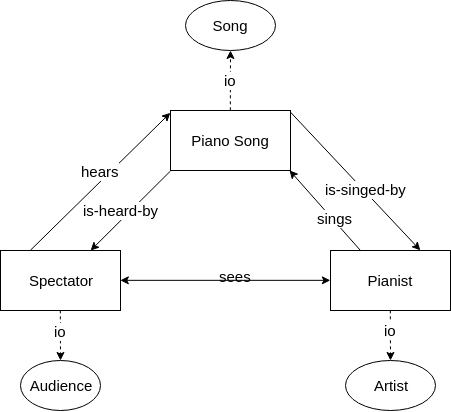
\includegraphics[width = 0.6\linewidth]{img/onto_example.png}
%         \caption{Exemplu de ontologie}
%     \label{fig:onto_ex}
% \end{figure}

'In \cite{Press2014AdrianApproach}, Adrian Groza identific'a practicile rele care trebuie evitate 'in design-ul ontologiilor. O prim'a practic'a defectuoas'a este utilizarea rela'tiei $is$ deoarece se poate produce confuzie 'intre rela'tia de apartenen't'a 'si rela'tia ce define'ste o subclas'a. Trebuie evitate rela'tiile inverse care nu sunt declarate 'si clasele care nu au indivizi. Clasele care de'tin un num'ar mult prea mare de subclase trebuie re-evaluate deoarece se poate realiza o nou'a ierarhie, mai specific'a. Indivizii nu trebuie trata'ti ca 'si clasele: unele elemente, cum ar fi un nume de ora's, trebuie tratate ca indivizi.

Diana Kalibatiene \cite{owl_languages} face o clasificare a limbajelor de implementare a ontologiilor. Sunt identificate dou'a categorii de limbaje pentru ontologii, 'si anume: limbaje tradi'tionale 'si limbaje bazate pe Web. 

Din prima categorie, a limbajelor tradi'tionale, face parte KIF\footnote{http://www-ksl.stanford.edu/knowledge-sharing/kif/}. Acesta este un limbaj cu semantic'a declarativ'a, este cuprinz'ator din punct de vedere logic. Pune la dispozi'tie defini'tii pentru obiecte, func'tii 'si rela'tii.

Din categoria a doua, a limbajelor destinate web-ului semantic, fac parte urm'atoarele:

\begin{itemize}
    \item OWL ({\it Web Ontology Language}) - include exprimarea conjunc'tiilor, a disjunc'tiilor, a variabileleor cuatificate universal. Acestea pot fi folosite pentru a ob'tine cunos'tin'te noi prin realizarea inferen'telor logice. Con'tine $OWL\ Lite$, $OWL\ DL$ 'si $OWL\ Full$ ca sublimbaje.
    \item RDF({\it Resource\ Description\ Language}). Este scris 'in XML 'si este destinat 'in'telegerii de c'atre calculatoare, nu de c'atre oameni. Resursele identificate sunt exprimate sub form'a de triple: subiect, predicat 'si un obiect. 
    \item OIL ({\it Ontology Interchange Language}) este bazat pe RDFS 'si DL. A fost creat pentru a fi 'in'teles 'in mod intuitiv de utilizatori. 
    \item DARPA Agent Markup Language (DAML) - const'a 'in dou'a p'ar'ti: limbajul ontologiei  'si un limbaj pentru exprimarea constr\ia ngerilor 'si pentru ad'augarea regulilor de inferen't'a.
\end{itemize}

'Intr-o ierarhie a limbajelor de dezvoltare a ontologiilor, OWL se afl'a mai sus ca RDF, reprezent\ia nd un nivel de expresivitate mai 'inalt ca RDF. OWL adaug'a semantic'a schemei 'si permite specificarea mai multor detalii despre propriet'a'ti 'si clase. Av\ia nd urm'atoarele axiome exprimate 'in DL:

\begin{tabular}{ll}
          &  {\it (A, B):\ ancestorOf}\\
          &  {\it (B, C):\ ancestorOf}\\
\end{tabular}

OWL, spre deosebire de RDF, va implica 'si axioma {\it (A, C): ancestorOf}. 

Pentru a genera concluzii din cuno'stin'tele valabile folosind tehncii logice precum deduc'tia, se folose'ste un ra'tionator. Pellet, Racer, HermiT sunt unele dintre sistemele disponibile pentru ra'tionare. Acestea sunt detaliate 'in sec'tiunea ~\ref{sec:pellet}.

Pentru ob'tinerea informa'tiilor din ontologie, este necesar'a utilizarea limbajelor de interogare specifice. Pentru interogarea ontologiilor dezvoltate 'in OWL, sunt cunoscute limbajele de interogare SQWRL 'si SPARQL. Printre limbajele de interogare utilizate pentru ontologiile dezvoltate cu RDF se num'ar'a: RQL, SeRQL 'si RDQL.



%%%%%%%%=================================
\subsection{Procesarea limbajului natural}

Limbajul natural este complex 'si divers, av\ia nd particularit'a'ti care difer'a de la limb'a la alta, de la o regiune la alt'a regiune. Procesarea limbajului natural 'incearc'a s'a g'aseasc'a o solu'tie pentru a ajuta sistemele computerizate s'a 'inteleag'a limbajul scris sau vorbit al unui om. 

'In procesarea limbajului natural, exist'a dou'a tehnici utilizate: {\it analiza\ sintactic'a} 'si {\it analiza\ semantic'a}.

Analiza sintactic'a se refer'a la modul 'in care sunt aranjate cuvintele 'intr-o propozi'tie astfel 'inc'at sa aib'a semns din punct de vedere gramatic. Aceasta este utilizat'a in procesarea limbajului natural pentru a studia 'in ce mod se aliniaz'a acesta cu regulile gramaticale. 'In acest context, sunt utiliza'ti algoritmi pentru a aplica regulile gramaicale unor propozi'tii 'in vederea deriv'arii unui 'in'teles din acestea. C'ateva procedee pentru analiza sintactic'a sunt: lemmatizarea, segmentarea, etichetarea p'ar'tilor vorbirii, parsarea 'si stemming-ul.

{\it Lemmatizarea} implic'a reducerea unui cuv\ia nt la forma de baz'a, din dic'tionar, a acestuia: 

\begin{center}
{\it Lemma("is") = be}
\end{center}

{\it Segmentarea} presupune divizarea textului 'in unit'a'ti precum cuvinte sau propozi'tii. 

{\it Etichetarea p'ar'tilor vorbirii} const'a 'in identificarea p'ar'tilor sintactice ale vorbirii pentru fiecare cuv\ia nt al propozi'tiei. De exemplu, pentru propozi'tia {\it What are the advantages of QLearn?}., felul 'in care p'ar'tile vorbirii sunt etichetate pot fi observate 'in tabelul ~\ref{table:pos_Tag}.


\begin{table}
\caption{Etichetarea p'ar'tilor vorbirii}
\centering                          % tabel centrat 
\begin{tabular}{|c|c|c|}          % 4 coloane centrate 
\hline\hline                        % linie orizontala dubla
Cuv\i ant& POS & Denumire\\ [0.5ex]   % inserare tabel
%heading
\hline                              % linie orizontal simpla
What & WP & pronume\\[1ex]    
are & VBP & verb persoana a 2-a singular\\[1ex]% [1ex] 
the & DT & determinant\\[1ex]
advantages & NNS & substantiv la plural\\[1ex]
of & IN & prepozi'tie\\[1ex]
QLearn & NNP & substantiv propriu \\[1ex]
\hline                              
\end{tabular}
\label{table:pos_Tag} 
\end{table}


\begin{figure}
    \centering
    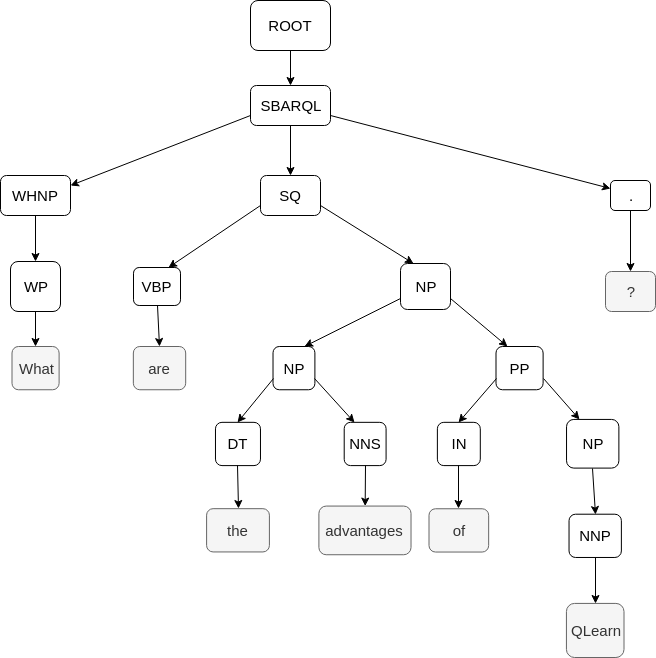
\includegraphics[width = 0.5\linewidth]{img/alice_parse.png}
        \caption{Exemplu de arbore sintactic}
    \label{fig:alice_parse}
\end{figure}

$Parsarea$ reprezint'a analiza automat'a a propozi'tiilor, 'tin\ia nd cont de strucura lor gramatic'a. Se atribuie etichete cu p'ar'ti de vorbire 'si se structureaz'a, 'in general, sub form'a de arbore sintactic. 'In figura ~\ref{fig:alice_parse} poate fi observat un exemplu al arborelui sintactic pentru propozi'tia {\it What are the advantages of QLearn?}.


$Stemming-ul$ const'a 'in reducerea cuvintelor la forma dat'a de r'ad'acina lor. Aceast'a form'a nu trebuie s'a reprezinte un cuv\ia nt valid.

Analiza semantic'a presupune extragerea 'in'telesului din text. Analiza semantic'a a textului cuprinde determinarea p'ar'tilor de text 'si asocierea unei categorii acestora, oferirea sensului unui cuv\ia nt pe baza contextului, utilizarea bazelor de date pentru a ob'tine rela'tii semantice 'si pentru convertirea 'in limbaj natural a acestora.


Procesarea limbajului natural sus'tine interac'tiunile 'intre om 'si sistemele informatice. Un avantaj al utiliz'arii limbajului natural pentru exprimarea cerin'telor este acela c'a utilizatorii nu sunt nevoi'ti s'a se adapteze unui anumit mod de utilizare sau limbaj al sistemului.

%%%%%%%================================
\subsection{Protocol de transfer}
HTTP ({\it HyperText\ Transfer\ Protocol}) este un protocol an nivelului aplica'tie destinat transferului de informa'tii pe internet.
Acesta utilizeaza URI ({\it Uniform\ Resource\ Indentifier}) pentru identificarea resurselor 'si pentru stabilirea unei conexiuni cu acestea. HTTP este bazat pe o arhitectura client-server 'si interschimba informa'tii de-a lungul uncei conexiunii sigure TCP/IP.

Informa'tiile interschimbate au denumirea de mesaje 'si pot fi request-uri sau r'aspunsuri. Un request este f'acut de un client c'atre server pentru a ob'tine informa'tii, iar r'aspunsul este un mesaj trimis de la server c'atre client ca urmare a request-ului. 

Un mesaj este format din antet 'si corp. 'In antetul mesajului sunt puse la dispozi'tie informa'tii despre request sau r'aspuns, sau despre datele con'tinute de corp. Antetele pot fi generale, pentru request-uri, pentru r'aspunsuri sau de tip entitate. Corpul mesajului con'tine datele transmise odat'a cu request-ul sau r'aspunsul 'si poate fi op'tional 'intr-un mesaj HTTP. 

Cele mai importante metode HTTP pentru request sunt $GET$, $POST$, $PUT$, $DELETE$.
 $GET$ este utilizat'a pentru a ob'tine informa'tii, acesta neav\ia nd niciun efect colateral asupra datelor.
 $POST$ este folosit pentru a trimite date c'atre server. Datele sunt con'tinute de corpul request-ului.
 Pentru a 'inlocui anumite date pe server se folose'ste $PUT$. 'In acest caz, resursele sunt identificate printr-un URI. $DELETE$ este utilizat pentru a 'sterge datele identificate de URI de pe server.
La acestea se mai adaug'a 'si altele: $HEAD$, $CONNECT$, $OPTIONS$, $TRACE$.

Ca r'aspuns, pe l\ia nga resursele identificate, un mesaj HTTP mai con'tine si codul de status care anun'ta cum s-a efectuat request-ul. Un cod $1xx$ este un cod care anun't'a c'a request-ul a fost primit 'si procesarea datelor continu'a. Codul $2xx$ anun't'a succesul request-ului. 'In cazul 'in care este necesar s'a se fac'a o alt'a ac'tiune ce cons't'a 'intr-o redirec'tionare pentru a se duce la cap'at request-ul, se va primi un cod de tipul $3xx$. Eroarea unui client, cum ar fi sintaxa incorect'a, se rezum'a la codul de eroare din seria $4xx$. O eroare de server, 'in care acesta nu a reu'sit s'a 'indeplineasc'a cerin'ta datorit'a unor probleme interne chiar dac'a request-ul este valid, este semnalat'a prin codurile $5xx$

HTTP reprezint'a un protocol de comunicare de 'incredere utilizat pentru a transmite date peste protocolul TCP/IP. O extensie a HTTP este HTTPS care reprezint'a o versiune sigur'a, 'in care datele transmise sunt criptate.


\subsection{Inteligen'ta artificial'a explicativ'a}

XAI ($Explainable\ Artificial\ Intelligence$) reprezint'a o tehnic'a prin care deciziile sau comportamnetul unui agent inteligent pot fi u'sor de 'inteles de oameni. A ap'arut ca necesitate 'impotriva sistemelor $black\ box$ care cauzeaz'a scepticism 'si ne'incredere 'in r\ia ndul utilizatorilor.

Potrivit DARPA \cite{darpaXAI}, un agent inteligent ar trebui s'a raspund'a la 'intreb'ari precum 
"{\it De\ ce\ ai\ f'acut\ asta?}", 
"{\it C\ia nd\ reu'se'sti?}", 
"{\it C\ia nd e'suezi?}", 
"{\it C\ia nd pot avea 'incredere 'in tine?}", 
"{\it Cum\ corectez o eroare?}". Programul $XAI$ dore'ste s'a creeze tehnici 'in special pentru machine-learning pentru a produce mai multe modele care pot fi explicate, p'astr\ia nd o bun'a performan't'a. Un alt obiectiv al acestui program este de a permite utilizatorilor s'a 'inteleag'a 'si s'a aib'a 'incredere 'in agen'tii inteligen'ti.

Explainable AI este esen'tial pentru a stabili 'increderea 'si a expune prin transparen'ta procesele care au loc pentru a genera un r'aspuns. Prin acesta, se poate garanta corectitudinea, iar utilizatorii pot 'intelege un output 'in func'tie de inputul utilizat.

\section{Tehnologii 'si unelte folosite}
\subsection{Angular}

Angular\footnote{Angular website https://angular.io/} este o unealt'a pentru construirea interfe'telor utilizator dinamice. Este u'sor de controlat 'si propune reutilizarea codului. Interfe'tele sunt construite pe baza HTML 'si TypeScript. 


% \begin{figure}
%     \centering
%     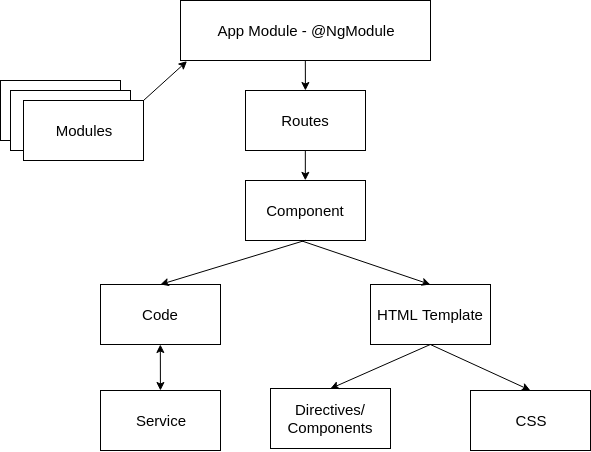
\includegraphics[width = 0.6\linewidth]{img/angular_schema.png}
%         \caption{Arhitectura unei aplica'tii Angular}
%     \label{fig:ang}
% \end{figure}


% O vedere de ansamblu a arhitecurii este prezentat'a 'in figura ~\ref{fig:ang} 'si este detaliat'a pe pagina oficial'a \cite{AngularCite}. 

Un $NgModule$ este cel mai de baz'a bloc al unei aplica'tii Angular, aceasta fiind definit'a de un set format din mai multe $NgModule$. Modulele sunt un context de compilare, func'tionalit'a'ti de baz'a, pentru componente. Pentru a forma unit'a'ti func'tionale, componentele sunt asociate cu codul corespunz'ator (servicii).

Prin rutare, se pot defini c'ai de navigare prin diferite st'ari ale aplica'tiei sau view-uri. 'In loc de a mapa c'aile URL spre pagini, un $Router$ le va mapa spre view-uri. Pentru a defini noi reguli de navigare, se asociaz'a cai de navigare componentelor. Se poate utiliza logic'a 'in program pentru a restric'tiona sau a alege ce view-uri vor fi afis'ate.

Componentele sunt structuri importante care definesc o clas'a destinat'a logicii 'si datelor aplica'tiei. O component'a este asociat'a unui template HTML care reprezint'a un view ce va fi afi'sat. Orice aplica'tie Angular con'tine cel pu'tin o component'a, aceasta fiind componenta r'ad'acin'a. Aceasta define'ste o ierarhie care con'tine toate celelalte componente.

Un template HTML este scheletul ce con'tine elementele grafice disponibile utilizatorului. Acesta poate s'a con'tina, pe l\ia nga cod HTML propriu-zis, 'si directive Angular sau alte componente refolosite. Template-ul HTML este stilizat cu ajutorul unui fi'sier CSS.

\subsection{Spring Boot}
Spring Boot\footnote{Spring Boot https://spring.io/projects/spring-boot} este un framework Java, open-source, utilizat pentru crearea de microservicii. Un microserviciu implic'a o arhitectur'a care permite developerilor s'a dezvolte servicii independent.

Cu ajutorul Spring Boot se poate realiza cu u'surin'ta inversiunea controlului prin injectarea dependen'telor, ceea ce duce la dezvolarea unei aplica'tii cu cuplare joas'a. Alte beneficii aduse de Spring Boot sunt u'surin'ta 'in managementul dependen'telor, auto configurarea, disponibilitatea unui container pentru servleturi inclus 'si utilizarea adnot'arilor.

Adnor'arile sunt unul din punctele forte ale framework-ului, acestea permit'and configurarea aplica'tiei cu u'surin't'a. $@SpringBootApplication$ se num'ar'a printre adnot'arile utilizate des. Se folose'ste 'in clasa ce reprezint'a punctul de start al aplica'tiei Spring Boot. Conform documenta'tiei oficiale \cite{springBootCite}, $@ComponentScan$ este utilizat pentru a semnala aplica'tiei care pachete con'tin clase ce ar trebui manageriate de Spring. Aceste clase pot include adnot'arile: 

\begin{itemize}
    \item $@Component$ - este utilizat sa denote o clas'a ca component'a. Astfel de clase sunt considerate $bean-uri$ 'si vor fi introduse 'in contextul aplica'tiei.
    \item $@Repository$ - este o specializare a adnot'arii $@Component$, fiind specific'a nivelului de $DAO$ al aplica'tiei. Excep'tiile ce sunt aruncate din nivelul de DAO vor fi traduse 'in $DataAccessException$, din Spring.
    \item $@Service$ - este o specializare a adnot'arii $@Component$ 'si nu pune la dispozi'tie alt comportament suplimentar fa't'a de aceasta. Este folosit'a pentru a exprima inten'tia de a realiza o clas'a din nivelul de service.
    \item $@Controller$ marcheaz'a o clas'a ca controller Spring MVC, fiind 'si aceasta o specializare a adnot'ariii $@Component$.
    \item $@RestController$ - este la baz'a o combina'tie 'intre $@ResponseBody$ 'si $@Controller$,  pentru a permite facilit'a'tile date de acestea dou'a.
\end{itemize}

Alte adnot'ari des utilizate sunt $@RequestBody$, $@ResponseBody$, $@Autowired$ 'si $@RequestMapping$. $@RequestBody$ indic'a faptul c'a parametrul metodei trebuie s'a fie legat de corpul request-ului web. $@ResponseBody$ este utilizat'a pentru a lega valoarea de return a metodei de corpul r'aspunsului dat de request-ul web. $@RequestMapping$ este folosit'a pentru a mapa request-urile web pe metode 'in clasele controller. Aceasta poate fi folosit'a at'at la nivel de clas'a, c\ia t 'si de metod'a, dar se prefer'a ca la nivel de metod'a se se foloseasc'a $@GetMapping$, $@PostMapping$, $@PutMapping$ sau $@DeleteMapping$. Adnotarea $@Autowired$ este utilizat'a pentru a injecta un bean 'intr-un atribut al clasei.

Fa'ta de framework-ul Spring original\footnote{Framework-ul Spring https://spring.io/}, Spring Boot pune la dispozi'tie autoconfigurarea. Acest lucru u'sureaz'a procesul de dezvoltare al aplica'tiei, ajung'and mult mai repede la un sistem executabil. Cu ajutorul $SpringBoot$, aplica'tia nu mai necesit'a a fi configurat'a prin XML, aceasta fiind auto-configurat'a prin adnot'ari.

\subsection{SPARQL}

SPARQL este un limbaj orientat pe date, acesta execut\ia nd interog'ari pe datele de'tinute 'intr-un model. Acesta identific'a informa'tiile pe baza constr\ia ngerilor 'si o returneaz'a sub forma de graf RDF sau a unui set de leg'aturi variabil'a-r'aspuns.

Potrivit \cite{sparql_tutorial}, o interogare SPARQL este format'a din declara'tii de prefix, definirea setului de date, clauza rezultatului, modelul de interogare 'si modificatori ai interog'arii.

Utilizarea operatorului $FILTER$ reprezint'a o practic'a 'int\ia lnit'a 'in interog'arile de tip SPARQL. Acesta permite restric'tionarea valorilor dintr-un r'aspuns. $FILTER$ are aceea'si func'tioalitate ca operatorul $LIKE$ din limbajul SQL. 

Un exemplu care utilizeaz'a ontologia $Friend\ of\ a\ Friend$\footnote{FOAF http://www.foaf-project.org/} 'si cuprinde $FILTER$ este relatat 'in exemplul ~\ref{ex:sparql_ex}.



\begin{example}[Interogare SPARQL]
\begin{lstlisting}[basicstyle=\footnotesize, numbers=left, firstnumber = 0]

PREFIX foaf:  <http://xmlns.com/foaf/0.1/>

SELECT ?email
WHERE {
    ?person foaf:mbox ?email .
    ?person foaf:name ?name.
    FILTER(?name = foaf:Mary).
} ORDER BY ASC(?email)
\end{lstlisting}
\label{ex:sparql_ex}
\end{example}

'In acest exemplu, linia (1) reprezint'a declara'tia de prefix a ontlogiei FOAF. Pe linia (3) este se afl'a clauza rezultatului, variabila rezultat pe care o dorim returnat'a este $?email$. Liniile (5)-(7) reprezint'a modelul de interogare: se interogheaz'a dup'a o persoan'a ($?person$) care are emailul ($foaf:mbox$) dat de variabila $?email$. Prin $FILTER$ se reduce mul'timea rezultatelor la acelea 'in care numele persoanei este $Mary$. Linia (8) prezint'a un modificator de interogare, astfel ca lista de email-uri rezultat'a s'a fie ordonat'a asccendent.

Cu ajutorul operatorului $FILTER$ se pot executa 'si opera'tii care implic'a operatorii logici $and$ 'si $or$. Pentru a exprima c'a numele este $Mary$ 'si emailul este $mary@mary.com$, se poate folosi construc'tia: 
\begin{center}
{\it FILTER(?name\ =\ foaf:Mary\ \&\&\ ?email\ =\ foaf:mary@mary.com)}
\end{center}

Dac'a dorim s'a c'aut'am o persoan'a care are numele $Mary$ sau $Alice$, constr\ia ngerea pentru $FILTER$ se rezum'a la:
\begin{center}
{\it FILTER(?name\ IN(foaf:Mary, foaf:Alice))}
\end{center} 

Pentru implementarea unei nega'tii, se utilizeaz'a operatorul $MINUS$, dar aceasta nu este unica variant'a. O interogare 'in care se cer persoanele care nu au numele $Mary$ este ~\ref{ex:ex_minus}.

\begin{example}[Interogare SPARQL care utilizeaz'a operatorul MINUS]
\begin{lstlisting}[basicstyle=\footnotesize, numbers=left, firstnumber = 0]

PREFIX foaf:  <http://xmlns.com/foaf/0.1/>

SELECT ?person
WHERE {
    ?person foaf:name ?name.
    MINUS( ?name = foaf:Mary).
} 
\end{lstlisting}
\label{ex:ex_minus}
\end{example}

'In exemplul men'tionat, se va construi mul'timea tuturor persoanelor $person$ cu numele $name$. Din aceas'ta mul'time se va sc'adea mul'timea celor care au numele $Mary$. Astfel rezult'a mul'timea persoanelor care nua u numele $Mary$. Diferen'ta mul'timilor implementat'a cu $MINUS$ conduce la o nega'tie.

'In plus fa't'a de aceste func'tionalit'a'ti descrise, limbajul SPARQL permite 'si inserarea utiliz\ia nd $INSERT$, updatarea utiliz\ia nd $UPDATE$ 'si 'stergerea datelor folosind $DELETE$.

Utilizarea limbajului de interogare SPARQL implic'a o serie de avantaje. SPARQL permite utilizatorilor s'a interoghezze date de tipul cheie-valoare, cum ar fi date RDF. SPARQL pune la dispozi'tie o serie de unelte pentru a combina r'aspunsurile mai multor scheme. Datorit'a faptului c'a ontologiile sunt puse la dispozi'tie extern, se pot utiliza prefixe f'ara a crea ambiguit'a'ti.

%%%%%%%=========================
\subsection{Protege}
Protege\footnote{Protege http://www.smi.stanford.edu/projects/protege/overview/index.html} este o platform'a disponibil'a pentru dezvoltarea aplica'tiilor bazate pe ontologii sau modele de domeniu. 

Editorul Protege-OWL\footnote{Protege OWL http://www.smi.stanford.edu/projects/protege/overview/protege-owl.html} este o extensie a originalului Protege. Acesta sus'tine dezoltarea 'in limbajul OWL. Acesta pune la dispozi'tie facilit'a'ti importante lucrului cu ontologii, cum ar fi: 'inc'arcarea 'si salvarea ontologiilor 'in diverse formate printre care 'si OWL, RDF, Turte, Manchester-OWL; editarea ierarhiei de clase 'si integrarea propriet'a'tilor; definirea sub forma de expresii OWL a caracteristicilor logice ale claselor; utilizarea ra'tionatoarelor 'si a limbajelor de interogare.

Interfa'ta utilizator grafica a editorului Protege-OWL permite pentru clase ad'augarea claselor echivalente, a subclaselor, crearea de instan'te 'si ad'augarea de clase disjuncte. 

Pentru un individ, Protege-OWL permite semnalarea faptului c'a acesta reprezint'a aceea'si instan't'a sau instan'te diferite cu un alt individ. 'In leg'atur'a cu un individ se pot ad'auga propriet'a'ti-obiect c'atre al'ti indivizi sau propriet'a'ti-dat'a c'atre valori.

Interogarea ontologiei dezvoltate se poate face cu ajutorul interog'arilor SPARQL sau DL 'si a regulilor SWRL sau SQRL. 'In timpul realiz'arii acestor interog'ari, pentru a ob'tine r'aspunsuri complete, este necesar ca un ra'tionator s'a fie activ. Utilizatorul poate face uz de urm'atoarele unelte de ra'tionare: HermiT, Pellet 'si Pellet (Incremental).

'In cadrul interfe'tei grafice, utilizatorul are posibilitatea de a vizualiza ontologia dezvoltat'a prin intermediul unor plugin-uri specifice: GraphViz\footnote{GraphViz https://www.graphviz.org/} 'si OntoGraph\footnote{OntooGraph https://github.com/NinePts/OntoGraph}.


RacerPro este o variant'a alternativ'a pentru Protege-OWL, dar aceast'a variant'a este pus'a la dispozi'tie sub form'a comercial'a. Test'and sistemul accesibil f'ar'a plat'a, am constatat c'a nu permite interog'ari SPARQL.



\subsection{Pellet}
\label{sec:pellet}

Pellet \cite{SirinPellet:Reasoner} este un ra'tionator pentru OWL-DL dezvoltat de Bijan Parsia et al. Este scris 'in Java, iar codul este open-source\footnote{Repository Pellet https://github.com/stardog-union/pellet} 'si de'tine exemple de utilizare. Ofer'a suport extins pentru ra'tionare cu indivizi folosind Jena sau interfe'te OW:-API. Acesta verific'a 'si consistent'a unui document OWL, retun\ia nd un raspuns de $consistent$, $inconsistent$ sau $necunoscut$.

Pellet cuprinde setul standard de servicii de inferen'ta in logic'a descriptiv'a, 'si anume: verificarea consisten'tei, satisfiabilitatea conceptelor, clasificare, realizare:
\begin{itemize}
    \item $Verificarea$ {\it consisten'tei} se asigur'a c'a ontologia nu con'tine fapte contradictorii.
    \item $Satisfiabilitatea$ $conceptelor$ verific'a dac'a exist'a posibilitatea pentru o clas'a s'a aib'a instan'te.
    \item $Clasificarea$ va crea 'intreaga ierarhie de clase pri verificarea tuturor rela'tiilor 'intre acestea. Acest serviciu permite g'asirea unui r'aspuns la interog'arile care implic'a 'si subclasele unei clase.
    \item $Realizarea$ poate fi utiliat'a dup'a $clasificare$ pentru a g'asi tipul direct sau toate tipurile fiec'arui individ, acesta fiind inclus 'in arborele clasific'arii.
\end{itemize}
   

Pentru a da un r'aspuns interog'arilor booleene, Pellet va reduce problema la una de insatisifiabilitate. 'In cazul 'in care un set de r'aspunsuri trebuie returnat, se vor calcula mai 'int\ia i r'aspunsurile evidente care constau 'in instan'te, iar apoi se caut'a non-instan'tele, 'incheind cu verficarea consisten'tei. 

Libr'aria Pellet con'tine un modul {\it Query\ Engine} pentru ABox pentru a r'aspunde interog'arilor conjunctive. Un major avantaj al acestui modul este c'a suport'a interog'ari 'in limbaj SPARQL sau RDQL.


'In \cite{tableau_alg} se aminte'ste c'a algoritmul $Tableau$ st'a la baza ra'tionatorului Pellet. Ra'tionatoarele dezvoltate pe baza algoritmului $tableau$ sunt dezvoltate pentru o logic'a mult mai expresiv'a. Astfel de ra'tionatoare 'incearc'a s'a construiasc'a un model consistent 'si satisfiabil utiliz\ia nd reguli de completare,'incerc\ia nd s'a extind'a modelul p\ia n'a satisface toate axiomele.
%  O alt'a categorie de reasonere, cele care folosesc reasoning determinat de consecin'te, sunt foarte bine optimizate pentru ontologiile OWL care con'tin logic'a Horn. Pentru ob'tinerea r'aspunsului, acestea aplic'a reguli de deducere pentru a infera  entailments (urm'arile) unor axiome din ontologie.

Conform \cite{SirinPellet:Reasoner} unde s-a realizat o compara'tie cu alte ra'tionatoare, Pellet func'tioneaz'a mai bine ca RacerPro, fiind testat pe 3 seturi de date pentru a ajunge la aceast'a concluzie. 'In compara'tie cu FaCT++ 'si cu RacerPro, Pellet nu este la fel de rapid 'in task-uri care implic'a ra'tionatoare pe TBox. 

Un avantaj major al libr'ariei Pellet 'in compara'tie cu RacerPro este acela c'a timpul de extragere al unui r'aspuns nu este influen'tat de dimensiunea r'aspunsului. 

HermiT este un alt ra'tionator pentru OWL 2 care suport'a interog'ari SPARQL. Comparativ cu acesta, Pellet a classificat mai multe ontologii comparativ cu HermiT. Datorit'a suportului extins 'si u'surin'tei de utilizare 'si integrare,  Pellet reprezint'a cea mai bun'a variant'a pentru realizarea extragerii r'aspunsurilor dintr-o ontologie personal'a. 


\subsection{RDFLib}

RDFLib\footnote{https://rdflib.readthedocs.io/en/stable/} este un package Python destinat proces'arii datelor 'in limbaj RDF, limbaj care reprezint'a datele sub form'a de graf. Reprezentarea datelor cu RDF este sub form'a de triple: subiect-predict-obiect. RDFLib are suport pentru interog'ari SPARQL 'si con'tine parsere 'si serializatoare pentru N-Triples, RDF/XML, N-Triples\footnote{https://www.w3.org/TR/n-triples/}, Turtle\footnote{https://www.w3.org/TR/turtle/}.

De mare interes este modulul $Graph$ al acestei libr'arii care pune la dispozi'tie reprezentarea triplelor RDF sub form'a de graf prin func'tia $parse()$. Pe aceste grafuri se pot realiza opera'tii cum ar fi: reuniune, diferen'ta 'sii intersec'tie. 'In plus fa'ta de aceste opera'tii, se pot face itera'tii pe graf.


RDFLib aduce cu sine o implementare a limbajelor SPARQL pentru interogare 'si update. Sunt puse dou'a func'tii, $query()$ 'si $update()$ la dispozi'tie pentru 'indeplinirea acestor avantaje. Func'tiile pentru interogare 'si update utilizeaz'a reprezentarea sub form'a de graf pentru a ob'tine r'aspunsuri. Aceste r'aspunsuri sunt sub forma de leg'aturi varibil'a-obiect.
\subsection{Quepy}

Quepy este un framework Python 2 destinat transform'arii 'intreb'arilor din limbaj natural 'in interog'ari care pot fi utilizate pentru baze de date sau ontologii. Acesta ofer'a suport petru limbajul de interogare SPARQL ($SPARQL\ Protocol\ and\ RDF\ Query\ Language$) 'si MQL ($Model\ Query\ Language$). 

Pentru o bun'a func'tionare a aplica'tiei, trebuie instalate 'in prealabil urm'atoarele libr'arii de care depinde Quepy:  $REfO$\footnote{REfO webpage https://pypi.org/project/REfO/}, $nltk$\footnote{nltk webpage http://www.nltk.org/}, $SPARQLWrapper$\footnote{SPARQLWrapper webpage https://pypi.org/project/SPARQLWrapper/} 'si, op'tional, $graphviz$\footnote{graphviz webpage http://www.graphviz.org/} pentru vizualizarea interog'arilor.
Conform, documenta'tiei acestui framework \cite{quepyCite}, trebuie parcur'si c\ia 'tiva pa'si pentru a realiza o aplica'tie Quepy. 

Libr'aria $REfO$ este utilizat'a pentru oferi suport expresiilor regulate pentru obiecte. Comparativ cu alte libr'arii destinate expresiilor regulate ce identific'a 'siruri de caractere, REfO este utilizat pentru a identifica secven'te arbitrare de obiecte. 

Libr'aria $nltk$ este o platform'a destinat'a aplica'tiilor Python pentru a interac'tiona cu limbajul natural. Pune la dispozi'tie resurse lexicale, dar 'si alte module pentru clasificarea, tokenizarea, etichetarea 'si parsarea propozi'tiilor 'in limbaj natural.

Libr'aria $SPARQLWrapper$ este un layer de interfa'tare pentru serviciile SPARQL. Aceasta este utilizat'a pentru transformarea 'si formatarea interog'arilor SPARQL intr-un format mai u'sor de 'in'teles.

Conform tutorialului oficial prezentat 'in documenta'tia Quepy, structura de baz'a a fiec'arui proiect Quepy con'tine urm'atoarele fi'siere: $parsing.py$, $dsl.py$, $settings.py$, $main.py$. 


'In $dsl.py$ se defineste limbajul specific al domeniului aplica'tiei, adic'a tabele, clase, rela'tii 'si caracteristici specifice unei baze de cuno'stin'te. Se pot folosi ca superclase urm'atoarele: $FixedDataRelation$ pentru a abstractiza o rela'tie c'atre o $Data$, $FixedRelation$ pentru a exprima rela'tia 'intre doua elemente, $FixedType$ pentru a abstractiza faptul c'a un element are un anumit tip, $HasKeyword$ pentru a decide care e cuv'antul cheie dup'a care vrem s'a selectam r'aspunsurile. 

'In exemplul ~\ref{ex:dsl}, folosind $FixedType$, $FixedRelation$ 'si un prefix $kb$ al unei ontologii despre ora'se, am definit doua clase 'in fi'sierul $dsl.py$: $IsPersonName$ 'si $HasAddress$.
\begin{example}[Clase din fisierul dsl.py]
\begin{lstlisting}[basicstyle=\footnotesize, language = Python]

class IsPersonName(FixedType):
    fixedtype = "kb:PersonName"
    
class HasAddress(FixedRelation):
    relation = "kb:has-address"
    reversed = True
\end{lstlisting}
\label{ex:dsl}
\end{example}

$IsPersonName$ define'ste o clas'a cu numele $PersonName$ din ontologia cu prefixul $kb$. $HasAddress$ define'ste o rela'tie fix'a $has-address$ a ontologiei date de prefixul $kb$, rolul variabile $reversed$ fiind de a folosi rela'tia invers'a.

Fi'sierul $parsing.py$ este folosit pentru definirea expresiilor regulate ce vor fi utilizate pentru a se potrivi cu 'intreb'arile 'in limbaj natural. Fiecare 'intrebare are asociat'a o clas'a 'in care expresiile regulate vor fi definite 'si interpretate apoi.

'In exemplul ~\ref{ex:parsing} am definit dou'a clase: $PersonName$ 'si $PersonHasAddress$. Acestea dou'a utilizeaz'a clasele $IsPersonName$ 'si $HasAddress$ din fi'sierul $dsl.py$.
\begin{example}[Clase din fisierul parsing.py]
\begin{lstlisting}[basicstyle=\footnotesize, language = Python]

class PersonName(Particle):
    regex = Pos("NN") | Pos("NNP")

    def interpret(self, match):
        name = match.words.tokens
        return IsPersonName() + HasKeyword(name)
    
class PersonHasAddress(QuestionTemplate):
    optional_opening = Question((Pos("WP") | Pos("WDT")) + Lemma("be") +
                    Pos("DT"))
    regex = optional_opening + Lemma("address") + \
             Pos("IN") + PersonName() + Question(Pos("."))

    def interpret(self, match):
        person = HasAddress(match.personname)
        return person, "enum"

\end{lstlisting}
\label{ex:parsing}
\end{example}

$PersonHasAddress$ define'ste expresia regulat'a pentru 'intrebarea:

\begin{tabular}{ll}
 & $What\ is\ the\ address\ of\ Maria?$
\end{tabular}


$Maria$ se potrive'ste cu expresia regulat'a definit'a de $PersonName$. Rezultatele selectate de interogare trebuie s'a fie nume de persoan'a 'si s'a aib'a cuv\ia ntul cheie $Maria$. Conform func'tiei $interpret$ din $PersonHasAddress$, rezultatele care pot fi date de interogare trebuie s'a aib'a o rela'tie invers'a de $has-address$ c'atre o persoan'a cu numele $Maria$.

'In continuare voi prezenta algoritmul ~\ref{alg:quepy} care reprezint'a fluxul de procesare al unei 'intreb'ari 'in cadrul aplica'tiei Quepy pentru a fi transformat'a 'in limbaj de interogare SPARQL.

  
\begin{algorithm}
\caption{Fluxul de procesare al unei 'intreb'ari folosind Quepy}
\label{alg:quepy}
 \KwData{Query $q$ in natural language}
 
 \KwResult{SPARQL query}
 
 $\mathcal{R} \leftarrow extractRules(\mathcal{Q})$\;
 
 $W_q \leftarrow tokenize(q)$\;
 
 $q_{SPARQL} = "\ "$\;

\ForEach {$r \in \mathcal{R}$}
{\If{$match(r, \mathcal{W}_q)$}{ 
\State $className = provenanceClass(r)$\; 
\State $graph[srcNode, (property, destNode)] = className.interpret(r, \mathcal{W}_q)$\;
\State $q_{SPARQL} = graphToSparql(graph)$
}        
%\EndIf
\textbf{return} $q_{SPARQL}$
}
\end{algorithm}


Inputul algoritmului este o 'intreare 'in limbaj natural, $q$. Primul pas const'a 'in extragerea tuturor regulilor definite 'in aplica'tie. Apoi, 'intrebarea utilizatorului este 'imp'ar'tit'a 'in tokeni, 'si i se atribuie etichete care identific'a ce parte a vorbirii este (substantiv, verb, prepozi'tie etc.), ob'tin\ia nd $W_q$. Rezultatul $q_{SPARQL}$ este 'ini'tializat. Pentru fiecare regul'a definit'a 'in mul'timea de reguli se verific'a dac'a se potrive'ste cu $W_q$. 'In cazul 'in care se potrive'ste, se ob'tine clasa 'in care a fost definit'a regula 'si 'in func'tie de metoda de interpretare, se adaug'a un noduri 'in graf care con'tin o tripl'a surs'a - proprietate - destina'tie. Se returnez'a interogarea SPARQL dup'a ce graful a fost interpretat. 'In cazul 'in care nu a fost indentificat'a o regul'a potrivit'a, se returneaz'a o interogare goal'a.

Potrivit analizei f'acute de Stein Seibu \cite{SteinSaebuOptiqueNLQF:Technologies}, framework-ul Quepy nu este scalabil, datorit'a necesit'a'tii de a introduce expresiile regulate manual. Pe de alt'a parte, un sistem care utilizeaz'a Quepy este mult mai u'sor de realizat fa't'a de celelalte proiecte asem'an'atoare: SINA \cite{Shekarpour2015SINA:Data} 'si Pythia \cite{Unger2011Pythia:Web}. Un alt avantaj al framework-ului Quepy este acela c'a este open source.


%%%%%%%%%%%%%%%%%%%%%%%%%%%%%%%%%%%%%%%%%%%%%%%%%%%%%%%%%%%%%%%%%%%%%%%%
\chapter{Proiectare de Detaliu 'si Implementare}
\label{sec:proiectare}

\section{Arhitectura sistemului}

'In cadrul acestei sec'tiuni se prezint'a o scurt'a descriere a aplica'tiei, iar 'in sec'tiunile urm'atoare vor fi prezentate pe larg fiecare dintre componente. Agentul explicativ pune la dispozi'tie o interfa'ta pentru utilizator 'in care acesta poate introduce 'intrebari, respectiv poate afla rezultatul acestora 'si termeni cheie ai ontologiei. Serverul asigur'a translatarea 'in limbaj de interogare SPARQL a 'intrebarii ini'tiale, rularea interog'arii prin metoda aleas'a de client 'si afi'sarea r'aspunsurilor 'in zona destinata acestuia.

Arhitectura agentului explicativ pe domeniul machine-learning este structurat'a pe niveluri, 'in care fiecare modul este independent si constituie un nivel. Acest lucru permite ca unele func'tionalit'a'ti s'a fie solu'tionate printr-o aplica'tie Java, iar altele cu ajutorul scripturilor Python. Figura ~\ref{fig:arch} ilustreaz'a arhitectura general'a a sistemului 'si maniera 'in care cele patru module comunic'a 'intre ele. 'In cadrul acestor componente, modulul serverului pentru inferen't'a joac'a un rol major, dac'a nu principal, toate apelurile provenite de la interfa'ta utilizator fiind procesate de acesta. Func'tionarea corect'a a serverului este esen'tial'a 'in aceast'a aplica'tie, dar 'si translatorul Quepy 'si ontologia asigur'a comportamentul adecvat al sistemului.

Interac'tiunea utilizatorului cu interfa'ta const'a 'in introducerea unei intreb'ari 'in limbaj natural 'si ac'tionarea comenzii pentru transformarea in limbajul de interogare SPARQL. Apelul va fi tratat de serviciul de inferen't'a {\it Reasoning Service}, prezentat 'in Fig. ~\ref{fig:arch}, care va realiza transformarea cu ajutorul translatorului Quepy, denumit 'in figura citata {\it Quepy translator}. Interogarea SPARQL va fi afi'sat'a 'si clientul are posibilitatea de a o modifica sau de a o executa fie folosind libraria Pellet, fie cu script-ul care utilizeaz'a RDFLib. R'aspunsul va fi prezentat 'in aria destinat'a. Utilizatorul mai are la dispozi'tie 'si o pagin'a 'in care poate solicita detaliile ontologiei: listarea claselor, a indivizilor 'si a propriet'a'tilor care le leag'a.


\begin{figure}
    \centering
    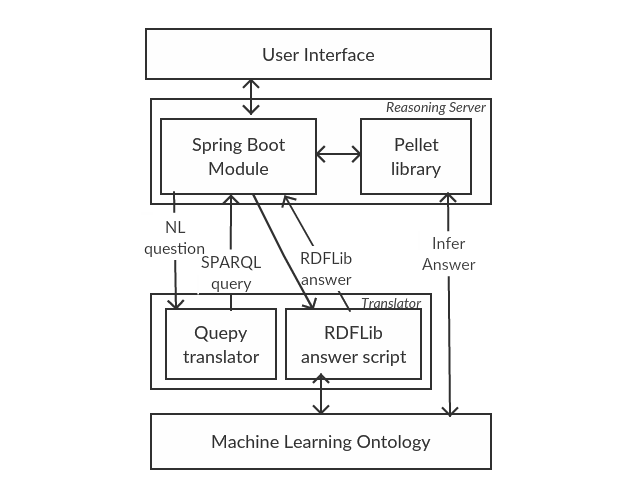
\includegraphics[width = 0.75\linewidth]{img/arhitectura-generala-black.png}
        \caption{Arhitectura sistemului}
    \label{fig:arch}
\end{figure}

Interfa'ta utilizator este construit'a simplu, 'in stil minimalist, astfel 'incat clientul s'a nu se piard'a 'in detalii. Este alc'atuit'a din dou'a pagini cu ajutorul c'arora utilizatorul poate chestiona datele 'in limbaj natural cu ajutorul librariei Pellet sau RDFLib sau poate ob'tine detalii despre ontologie. 

Serverul pentru inferen't'a, 'in imaginea mai sus men'tionat'a {\it Reasoning Service}, este consituit din libr'aria Pellet 'in care am integrat un modul Spring Boot pentru a pune la dispozi'tie sub form'a de endpoint-uri func'tionalit'a'tile necesare. Ca arhitectur'a, este format dintr-un nivel de control, un nivel de  servicii pentru ob'tinerea informa'tiilor de la libr'aria Pellet si de la modulul Python care utilizeaz'a RDFLib, 'si un nivel inferior pe care se afl'a libr'aria pentru inferen't'a.

Pe cel de-al treilea nivel al arhitecturii generale este pozi'tionat modulul Python denumit {\it Translator}. Acesta are doua func'tionalit'a'ti, o func'tionalitate pentru translatarea 'intreb'arilor din limbaj natural 'in SPARQL 'si una pentru interogarea ontologiei folosind libr'aria RDFLib. Translatorul Quepy este generat automat cu ajutorul framework-ului Quepy 'si con'tine clasele standard pentru parsare, pentru 'in'telegerea limbajului specific al domeniului 'si pentru ini'tializarea aplica'tiei. La acestea, se adaug'a un script pentru ob'tinerea unui r'aspuns cu ajutorul libr'ariei RDFLib.

Nivelul inferior const'a 'in ontologie, reprezent'and componenta care asigur'a persisten'ta datelor referitoare la machine learning. Indivizii acesteia sunt structura'ti 'in clase si subclase, depinz\ia nd unul de altul prin propriet'a'ti. O detaliere a arhitecturii ontologiei, c\ia t 'si a func'tionalita'tii 'si implement'arii fiec'arei componente mai sus amintite, va fi prezentat'a 'in cardul acestui capitol, 'in sec'tiunile care urmeaz'a. 

'In Figura~\ref{fig:arch_det} se prezint'a modulele principale ale sistemului, 'impreuna cu modul detaliat de comunicare al acestora. Fluxul de informa'tii porne'ste de la utilizator 'si str'abate serverul pentru inferen't'a, {\it Reasoning Server}. 'In situa'tia 'in care s-a f'acut un apel pentru translatarea unei 'intreb'ari din limbaj natural 'in SPARQL sau pentru ob'tinerea r'aspunsului prin RDFLib, este utilizat 'si modulul {\it Translator}, 'in fun'tie de cerin'te. 

\begin{figure}
    \centering
    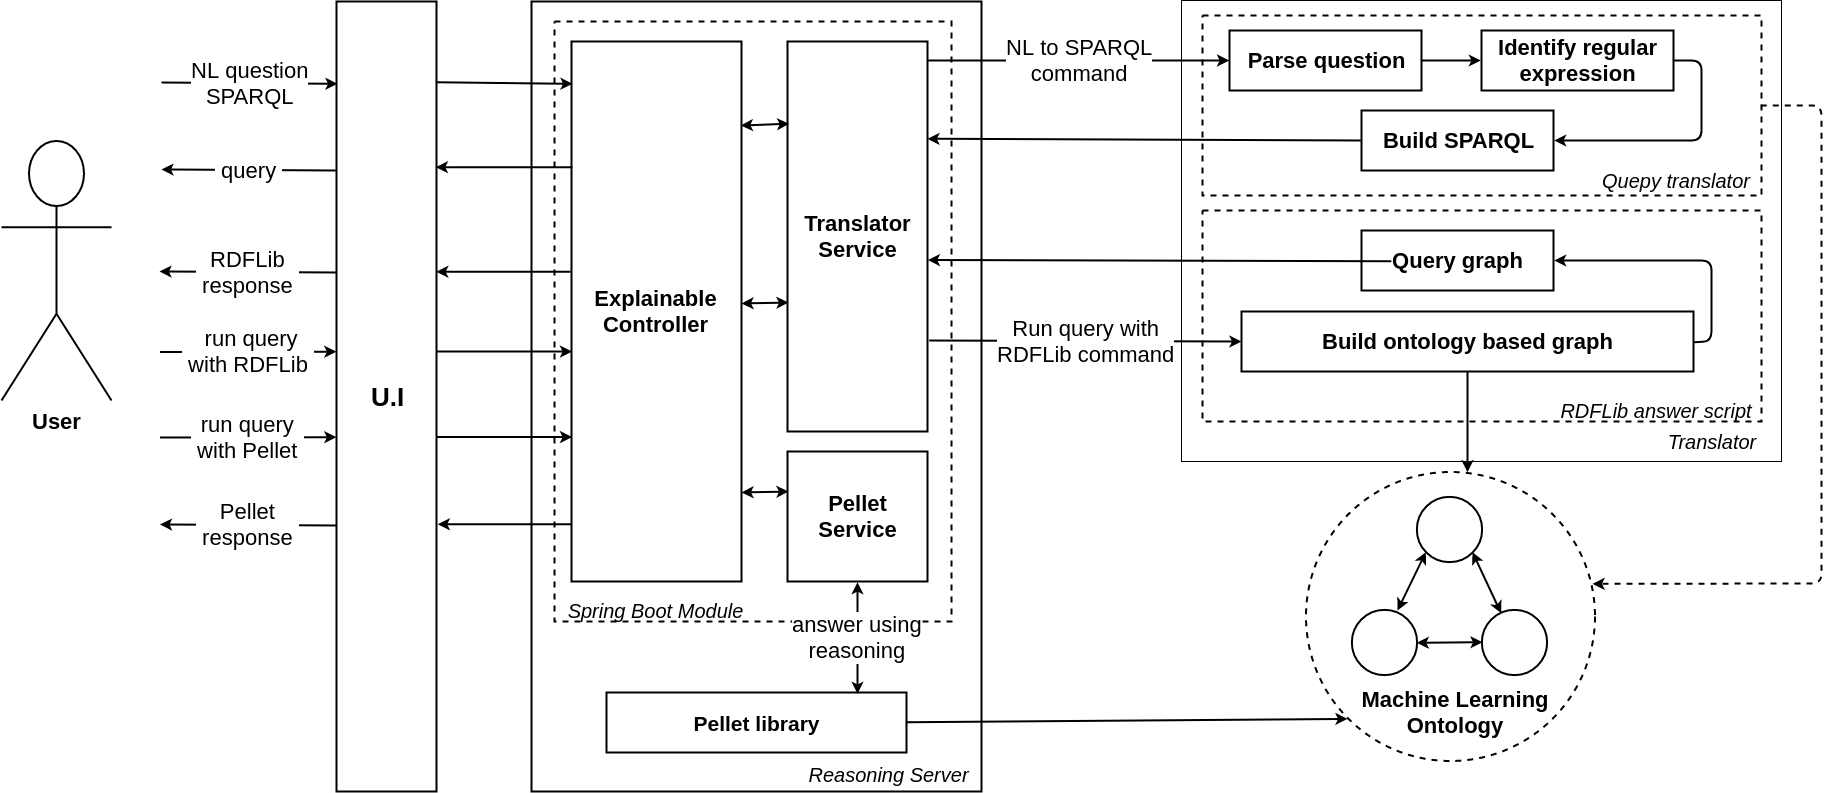
\includegraphics[width = 0.9\linewidth]{img/architecture_details.png}
        \caption{Elemente de comunicare 'in arhitectur'a}
    \label{fig:arch_det}
\end{figure}

Imaginea mai sus amintit'a pune 'in valoare trei situa'tii principale, care sunt folosite 'in mod global: translatarea unei 'intrebari 'in SPARQL cu ajutorul libr'ariei Quepy, interogarea r'aspunsului prin Pellet sau prin RDFLib. 'In toate aceste cazuri, se utilizeaz'a ontologia 'incarcat'a in memoria aplica'tiei sau se face uz de abstractizarea acesteia 'in cod, pentru modulul translatorului Quepy.

Primul pas al utilizatorului este de a insera 'intrebarea si de a activa apelul translat'arii acesteia. Serverul constituit din modulul Spring Boot va intercepta cerint'a 'in {\it Explainable Controller} 'si o va trece mai departe la serviciul dedicat, {\it Translator Service}. Acesta din urm'a execut'a comanda de rulare a modulului {\it Quepy translator}. Translatorul parseaz'a 'intrebarea, identific'a expresia regulat'a cu care se potrive'ste 'si contruie'ste interogarea SPARQL dintr-un graf generat de acest proces, apoi pune la dispozi'tie r'aspunsul pentru a fi preluat de {\it Reasoning Server}. Ca r'aspuns al apelului f'acut de utilizator, serverul va returna interogarea, iar aceasta va fi afi'sat'a 'in interfa'ta utilizator.

De'si primul pas poate fi omis 'si clientul poate s'a introduc'a manual interogarea pe care o dore'ste, rularea interog'arii aferente 'intreb'arii utilizatorului constituie al doilea pas logic 'in execu'tia cerin'tei. Utilizatorul activeaz'a comanda pentru rulare cu Pellet sau cu RDFLib din interfa'ta utilizator. 'In ambele cazuri, 'si atunci c'and dore'ste aflarea r'aspunsului prin inferen'ta sau prin extragere din graf, apelul va fi recep'tionat de controller. 

Dac'a ne afl'am 'in situa'tia 'in care se dore'ste aflarea r'aspunsului prin Pellet, controllerul  va 'inainta cererea la {\it Pellet Service}. Acesta o va solu'tiona cu ajutorul libr'ariei Pellet care de'tine modelul ontologiei 'in memorie 'si va extrage r'aspunsul prin ra'tionare. Astfel, 'si solu'tiile mai pu'tin evidente vor fi incluse 'in r'aspuns. R'aspusul este formatat de c'atre {\it Pellet Service} 'in format JSON pentru o lizibilitate crescut'a.

Solu'tionarea r'aspunsului prin graful RDFLib const'a in 'inaintarea apelului c'atre script-ul de ob'tinere a r'aspunsului bazat pe RDFLib, implementat 'in {\it Translator}. Pentru aflarea r'aspunsului, aceasta func'tie va citi ontologia sub form'a de graf RDF de la locatia precizat'a. Acest model RDF al ontologiei va fi interogat cu ajutorul query-ului transmis ca parametru 'si va returna un JSON cu rezultatele. Serviciul responsabil cu preluarea rezultatului este {\it Translator Service}. Acesta va returna controllerului rezultatul, care mai departe le va transmite interfe'tei utilizator, unde vor fi afi'sate.

Aplica'tia prezentat'a are o arhitectur'a structurat'a pe niveluri, oferind independe't'a 'intre module. Acest fapt aduce cu sine avantaje cum ar fi: func'tionarea aplica'tiei pe baza interogarilor directe 'in SPARQL 'in cazul 'in care modulul {\it Translator} nu func'tioneaz'a; 'inlocuirea ontologiei cu alta dintr-un domeniu diferit; asignarea atribu'tiilor clare 'si separate modulelor. 




\section{Modulul interfe'tei utilizator}

O necesitate a acestei aplica'tii, datorit'a nevoii interac'tiunii unor utilizatori cu aceasta, a fos tinterfa'ta utilizator. Aceasta a fost implementat'a pentru a ajuta clien'tii 'in realizarea opera'tiilor sistemului implementat. Interfa'ta utilizator este implementat'a 'in Angular, fiint constituit'a din doua componente principale, fiecare component'a reprezent\ia nd o pagin'a.

O caracateristic'a cheie a acestei interfe'te este transparen'ta 'in pasii efectua'ti. Astfel, interfa'ta utilizator sus'tine $Exaplainable\ AI$. Datorit'a nevoii de explicare a unui agent inteligent, pentru ca utilizatoriii s'a 'in'teleag'a de ce primesc anumite rezulate 'si de unde provin acestea, am realizat o interfa'ta care sa permit'a utilizatorului sa vizualizeze toate clasele ontologiei, to'ti indivizii acesteia 'si toate regulile.

Interfa'ta utilizatorul pune la dispozi'tie doua pagini responsabile pentru 'indeplinirea cerin'telor sistemului. O prima pagin'a permite utilizatorului inserarea unei cerin'te 'in limbaj natural. Datorit'a nevoii explic'arii unui r'aspuns dat, conform $Explainable\ AI$, am introdus un pas suplimentar pentru afis'area interog'arii SPARQL. Astfel, utilizatorul in'telege una din etapele algoritmului de extragere a r'aspunsului. Acesta poate s'a editeze interogarea, ceea ce ofera flexibilitate 'in extragerea r'aspunsului. 'In aceast'a pagin'a se pune la dispozi'tie op'tiunea de a interoga ontologia cu ajutorul libr'ariei Pellet sau prin RDFLib. R'aspunsul este afi'sat intr-o caset'a special destinat'a.

A doua pagin'a pus'a la dispozi'tie de interfa'ta utilizator permite interogarea tuturor claselor, a indivizilor si a regulilor ontologiei, 'in 'incercarea de a familiariza utilizatorul cu termenii specifici con'tinu'ti de aceasta. Acesta este tot un pas spre $Explainable\ AI$, pentru ca utilizatorii s'a 'inteleag'a deciziile agentului.

Prin intermediul interfe'tei utilizator, clientul poate folosi aplica'tia u'sor 'si sigur, fiind 'in'stiin'tat prin alerte 'in cazul in care 'intrebarea introdus'a nu este corect'a, interogarea SPARQL nu este una valid'a sau a ap'arut o eroare pe parcurs. Interfa'ta utilizator ofer'a un mediu controlat pentru folosirea aplica'tiei.

\section{Modulul de raspuns bazat pe ra'tionare 'in logic'a de descriere}

{\it Reasoning Server} reprezint'a punctul central al aplica'tiei, fiind modulul care rezolv'a cererile utilizatorilor. Acesta este un modul Spring Boot, integrat 'in libr'aria Pellet\footnote{https://github.com/stardog-union/pellet}, ce deleag'a componentele spre a 'indeplini sarcinile cerute de utilizator. 'In figura~\ref{fig:uml_server} este prezentat'a o parte important'a a serverului, respectiv clasele implementate de mine 'impreuna cu cele din libr'aria Pellet de care depind.
\begin{figure}[h!]
    \centering
    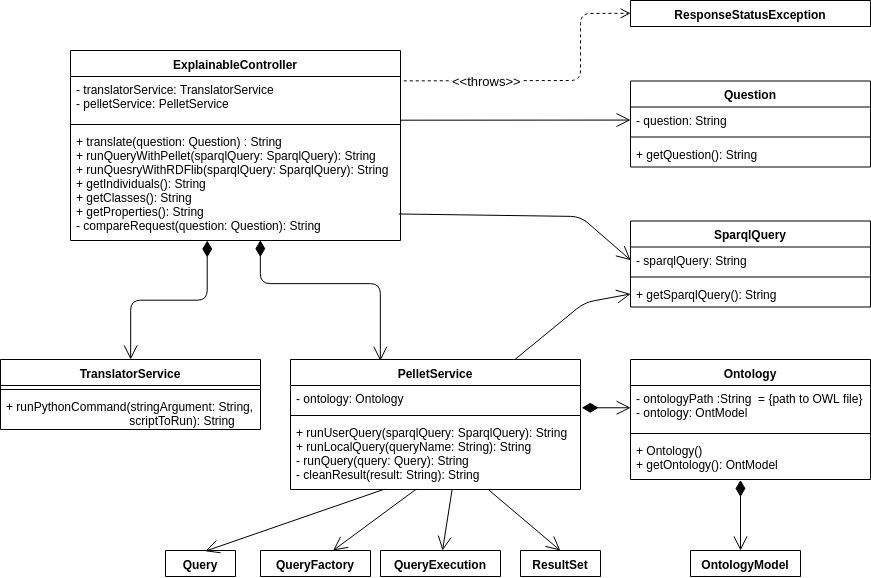
\includegraphics[width = 0.9\linewidth]{img/uml_server.png}
        \caption{Diagrama de clase a serverului {\it Reasoning Server}}
    \label{fig:uml_server}
\end{figure}

'In diagrama din figura ~\ref{fig:uml_server}, {\it ExplainableController} 'indepline'ste func'tia de controller al aplica'tiei. Este format din $translatorService$ 'si $pelletService$ a c'aror instan'te sunt aduse prin injectarea dependin'telor. Acestea au rolul de 'indeplinire a serviciilor, respectiv a logicii mai complexe pentru ob'tinerea r'aspunsurilor. $PelletService$ con'tine o instan't'a a ontologiei, $ontology$. Aceasta, la r\ia ndul ei este ob'tinut'a cu ajutorul fi'sierului OWL 'si a modelului pus la dispozi'tie de Pellet, $OntModel$. 'In plus fa't'a de $Ontology$, consider c'a clasele $Question$, $SparqlQuery$ sunt alte doua clase ce apar'tin modelului aplica'tiei, fiind utile 'in 'incapsularea datelor din request-uri.

$Query$ 'si $QueryFactory$ abstractizeaz'a o interogare 'in forma SPARQL care urmeaz'a a fi utilizat'a de Pellet pentru a ob'tine un r'aspuns de tipul $ResultSet$ prin intermediul $QueryExecution$. Acestea sunt clase care fac parte din libr'aria Pellet 'si nu le vom detalia.

Metoda $translate$ este apelat'a prin intermediul endpoint-ului {\it /translateQuery} 'si con'tinutul datelor transmise este un obiect din clasa $Question$, fiind o abstractizare a 'intreb'arii utilizatorului. Este utilizat'a pentru translatarea 'intreb'arii din limbaj natural 'in limbaj de interogare SPARQL.  Dac'a prin 'intrebare utiliztorul solicit'a compararea a doi algoritmi, se va utiliza metoda $compareRequest$ 'si se va returna o interogare SPARQL construit'a local. Altfel, aceasta apeleaz'a metoda $runPythonCommand$ din $TranslatorService$ 'si returneaz'a rezultatul dat de Quepy c'atre interfa'ta utilizator. Asem'an'ator, $runQueryWithRDFLib$ din controller este atins'a prin intermediul rutei {\it /runQueryWithRDFLib} 'si apeleaz'a aceea'si metod'a pentru rulare a comenzii , preciz\ia nd de data aceasta script-ul de ob'tinere a r'aspunsului cu RDFLib.

Metoda $runQueryWithPellet$ este folosit'a pentru ob'tinerea r'aspunsului la interogarea SPARQL print intermediul Pellet. Utilizeaz'a path-ul {\it /runQueryWithPellet} 'si va apela $runUserQuery$ din $PelletService$. 'In $runUserQuery$ se stabile'ste interogarea SPARQL a utilizatorului 'si se apeleaz'a $runUserQuery$. Prin $runQuery$, r'aspunsul este ob'tinut de la Pellet 'in format JSON utiliz'and clasele $QueryExecution$ 'si $ResultSet$, urm'and ca apoi acesta s'a fie cur'a'tat de prefixuri prin intermediul metodei $cleanResult$.

Metodele $getClasses$, $getIndividuals$ 'si $getProperties$ sunt accestate prin intermediul path-urilor $/classes$, $/individuals$ 'si respectiv $/properties$. Acestea au rolul de a ob'tine toate clasele ontolgiei, to'ti indivizii 'si toate propriet'a'tile. Utilizeaz'a metoda $runLocalQuery$ 'si interog'ari 'in limbaj SPARQL definite local. Pentru ob'tinerea r'aspunsului se folose'ste metoda $runQuery$, asem'an'ator cazului 'in care se utilizeaz'a interogarea utilizatorului.

Libr'aria Pellet reprezint'a suportul pentru modulul $Reasoning\ Server$ 'si realizeaz'a ob'tinerea r'aspunsului prin inferen'ta 'in logic'a descriptiv'a. Prin intermediul $Explainable$ $Controller$, utilizatorul are acces la translatarea din limbaj natural 'in limbaj de interogare SPARQL, c'at 'si la interogarea ontologiei prin Pellet sau prin RDFLib.

Sistemul este dezvoltat astfel 'inc\ia t sa permit'a 'intreruperea cursului aplica'tiei prin aruncarea excep'tiilor 'in cazul 'in care apar evenimente nedorite. Dac'a translatarea interog'arii din limbaj natural 'in limbaj de interogare SPARQL este defectuoas'a, sau dac'a interogarea SPARQL care se folose'ste pentru a chestiona ontologia prezint'a anomalii, din controller se arunc'a $ResponseStatusException$. Aceasta este o clas'a customizat'a pentru a 'ingloba statusul r'aspunsului, c'at 'si motivul 'intreruperii. 'Si 'in alte cazuri, cum ar fi 'in cazul c'ampurilor goale, se arunc'a aceast'a excep'tie, cu un mesaj corespunz'ator.

\section{Modulul de raspuns pe baza de graf}

Acest modul este destinat interog'arii ontologiei aflat'a 'in forma de graf RDF 'si folose'ste RDFLib pentru a pune 'in practic'a acest lucru. Utilizarea libr'ariei RDFLib este simpl'a, fiind necesar'a doar instalarea 'si importarea acesteia. Modulul 'in care am implementat interogarea ontologiei 'in format RDF este un script 'si vine 'in ajutor pentru momentele 'in care un query SPARQL are anumite particularit'a'ti semantice care nu sunt interpretate 'in acela'si mod de Pellet. 

\begin{figure}
\centering
\begin{lstlisting}[language=Python, basicstyle=\footnotesize,numbers=left, xleftmargin=.05\textwidth]
import json, re, sys
from rdflib import Graph

PREFIXES = ["http://www.semanticweb.org/machine-learning-ontology#",  
            "http://www.w3.org/2002/07/owl#"]


def to_json(query_response):
    list_result = []
    for row in query_response:
        dictionary_response = {}
        for i in range(len(row)):
            current_result = row[i]
            for prefix in PREFIXES:
                if prefix in row[i]:
                    current_result = re.sub(prefix, "", row[i])
            index = row.labels.keys()[row.labels.values().index(i)]
            dictionary_response[index] = current_result
            list_result.append(dictionary_response)

    json_result = json.dumps(list_result, sort_keys=False, indent=4)
    return json_result


query = sys.argv[1]
g = Graph()
g.parse(r'../ontologies/machine-learning-ontology.owl', format="xml")
query_response = g.query(query)
json_result = to_json(query_response)
print json_result

\end{lstlisting}
        \caption{Scriptul pentru interogare prin RDFLib}
      \label{fig:rdflib_script}
\end{figure}

'In figura~\ref{fig:rdflib_script} primul pas 'in ob'tinerea unui r'aspuns la o interogare SPARQL este de a citi de la linia de comand'a interogarea SPARQL care a fost transmis'a, 'in cazul aplica'tiei noastre, de c'atre serviciul aferent din {\it Reanoning Service}. La liniile (26)-(25), se formeaz'a un graf 'si ontologia noastr'a este parsat'a si salvat'a sub forma de noduri de triple. 'In continuare, la linia (28), se afl'a r'aspunsul interog'arii SPARQL. R'aspunsul dat de RDFLib nu este compatibil cu formatul JSON 'si con'tine informa'tii despre prefixe care ar putea induce 'in eroare utilizatorul. Astfel c'a, am implementat func'tia $to\_json(query\_response)$, ilustrat'a 'in figura~\ref{fig:rdflib_script} la liniile (8-22), pentru a transforma r'aspunsul in format JSON 'si a-l 'infrumuse'ta. 

'In final, raspunsul $json\_result$ va fi printat 'si preluat de c'atre server. Dup'a cum am mai amintit 'in acest capitol, r'aspunsul este trimis de c'atre server la interfa'a utilizator, unde va fi vizualizat de c'atre client.


\section{Modulul de translatare}
\subsection{Arhitectura 'si func'tionarea translatorului Quepy}

Modulul $Translator$ este construit 'in Python cu ajutorul framework-ului Quepy. Este destinat pars'arii 'si translat'arii 'intreb'arilor din limbaj natural 'in limbaj de interogare SPARQL. Aceste interog'ari SPARQL sunt utilizate pentru a interoga ontologia despre $machine-learning$. Modulul este generat automat de o comand'a quepy, iar 'in figura ~\ref{fig:quepy_files} se pot observa componentele necesare modulului $Translator$ de care facem uz 'in aceast'a aplica'tie. 
\begin{figure}
    \centering
    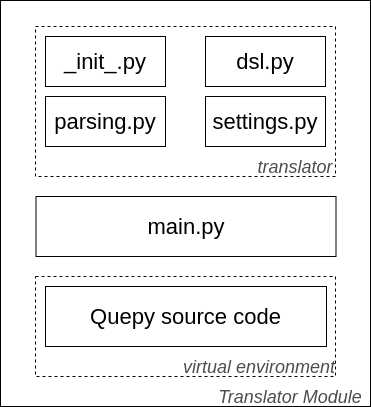
\includegraphics[width = 0.5\linewidth]{img/quepy_schema.png}
    \caption{Componentele modulului $Translator$}
    \label{fig:quepy_files}
\end{figure}

Fi'sierul $\_init\_.py$ constituie punctul de plecare al aplica'tiei, fi'sierul de ini'tializare. 'In acesta se import'a fi'sierul $parsing.py$, iar la instalarea aplica'tiei va fi citit prin intermediul $\_init\_.py$. 

Unul dintre cele mai importante fi'siere ale acestui modul este $parsing.py$. Acesta con'tine toate regulile de parsare ale aplica'tiei. 'In acest fi'sier sunt declarate toate 'intreb'arile permise de sitemul nostru, sub forma de patternuri. 'In sec'tiunea ~\ref{sec:parse} vom detalia acest fi'sier, 'impreuna cu procedeul de dezvoltare.

Fi'sierul $settings.py$ presupune locul 'in care se declara toate prefix-urile necesare unei interog'ari SPARQL, cum ar fi 'in cazul nostru prefixul pentru ontologia noastr'a 'si altele. Tot 'in acest loc, se decide limbajul de interogare, care 'in modulul $Translator$ este SPARQL.

Limbajul specific al domeniului este definit in $dsl.py$, fi'sier 'in care am adaugat toate clasele ontologiei noastre, 'impreuna cu propriet'a'tile acestora. Modul de detaliere al ontologiei, exemple de clase din acest fi'sier 'si o descriere mai larga a acestuia sunt 'in sec'tiunea ~\ref{sec:dsl}. 

Fi'sierul $main.py$ con'tine logica de pornire a aplica'tiei. 'In acesta am apelat ini'tializarea translatorului, am citit 'intrebarea utilizatorului din argumentele liniei de comand'a 'si am solicitat transformarea acesteia 'in SPARQL. 
Datorit'a faptului c'a am modificat 'si unele elemente ale libr'ariei pentru a implementa operatorii logici, este 'si aceasta reprezentat'a 'in imagine, 'in mediu virtual creat la formarea aplica'tiei.

$Translatorul$ este unul dintre cele mai importante module ale sistemului nostru, efectu\ia nd transaltarea din limbaj natural 'in limbaj de interogare SPARQL. Dupa ce utilizatorul introduce o 'intrebare 'in limbaj natural 'si cere traducerea sa 'in SPARQL, modulul este ini'tializat. 'In acest pas, toate regulile definite de noi 'in fi'sierul $parsing.py$ sunt 'inregistrate spre a fi folosite. 
'Intrebarea utilizatorului este 'imp'ar'tit'a 'in cuvinte 'in func'tie de partea de vorbire pe care o reprezint'a. Se decide c'arei reguli se supune 'intrebarea adresat'a. Odat'a identificat'a regula, se folosesc clasele 'si regulile ontologiei definite 'in $dsl.py$ pentru a construi o interogare SPARQL restric'tionat'a de modul de interpretare decis de noi. 


\subsection{'Incorporarea elementelor ontologiei 'in Quepy}
\label{sec:dsl}

Pentru a putea construi interog'ari potrivite pentru o ontologie, modulul Quepy trebui customizat pentru a cunoa'ste clasele 'si propriet'a'tile din ontologie, c\ia t 'si alte reguli care sunt necesare a fi integrate 'in interog'ari. 'In fi'sierul $dsl.py$ am definit clasele asem'an'ator list'arii de cod~\ref{lst:learning_meth_op}: 
\begin{lstlisting}[basicstyle=\footnotesize, language = Python, label = lst:learning_meth_op, caption = Clasa LearningMethod]
   class IsLearningMethod(FixedType):
    fixedtype = "ml:LearningMethod"

    def __init__(self, operator):
        super(IsLearningMethod, self).__init__(operator)
        self.fixedtype = operator + "ml:LearningMethod"

\end{lstlisting}

Acesta este un exemplu 'in care am 'incadrat 'si 'imbun'at'a'tirile aduse libr'ariei, 'si anume suportul pentru o operatorii logici. Propriet'a'tile sunt definite asem'an'ator cu list'arii de cod~\ref{lst:learning_meth_rel}:

\begin{lstlisting}[basicstyle=\footnotesize, language = Python, label = lst:learning_meth_rel, caption = Proprietatea has-learning-method]
class HasLearningMethodReversed(FixedRelation):
    relation = "ml:has-learning-method"
    reverse = True

class NotHasLearningMethod(MinusFixedRelation):
    relation = "ml:has-learning-method"
    reverse = False

class HasLearningMethod(FixedRelation):
    relation = "ml:has-learning-method"
    reverse = False

\end{lstlisting}

'In acest exemplu am 'incadrat rela'tia invers'a, rela'tia implementat'a de mine pentru a sus'tine operatorul $MINUS$ cu func'tia de $not$, 'si rela'tia simpl'a.


\subsection{Parsarea 'intreb'arilor}
\label{sec:parse}

'In fisierul $parsing.py$ am definit toate regulile de parsare ale 'intreb'arilor, un num'ar total de 15 clase asociate ficare c\ia te unei 'intreb'ari. Acestea con'tin regulile de parsare, 'impreuna cu o metod'a $interpret$ care specific'a ordinea 'in care vor fi ad'augate elementele identificate 'in interogare. 

Figura ~\ref{fig:r1} detaliaz'a regula pentru identificarea indivizilor clasei $Algorithm$. 'In aceast'a regul'a, $target$ func'tioneaz'a ca 'inlocuitor pentru conceptul c'aruia dorim s'a 'i afi'sam indivizii. Poate fi substantiv (NN), substantiv propriu (NNP) sau substantiv la plural (NNS). Variabila $optional\_opening$ este un 'inlocuitor pentru {\it"What are the"} sau {\it"Which are the"} 'si este op'tional'a, a'a cum este definit de comportamentul func'tiei $Question$. Prin $Lemma("be")$ 'in'telegem cuv\ia ntul de baz'a 'si inflexiunile sale, adic'a toate formele verbului $"to\ be"$. 'In exemplul~\ref{fig:r1} sunt prezentate expresiile regulate pentru identificarea 'intreb'arii.
Expresiile $regex1$ 'si $regex2$ sunt cuprinse 'in $regex$ 'si reprezint'a toate formele acceptate ale acesteia.

\begin{figure}[h]
\centering
\begin{lstlisting}[basicstyle=\footnotesize, numbers=left, xleftmargin=.05\textwidth]
target = Group (Pos("NN") | 
                Pos("NNP") | 
                Pos("NNS"), "target")
                
opt_opening = Question((Pos("WP") | 
                        Pos("WDT")) + 
                          Lemma("be") + 
                          Pos("DT"))
                          
regex1 = optOpening + 
         Question(Lemma("individual") | 
                  Lemma("instance")) + 
                    Pos("IN") + target + 
                    Question(Pos("."))
                    
regex2 = Question(Lemma("list") | 
                  Lemma("show") | 
                  Lemma("print")) + target +   
                  Question(Lemma("individual") |
                           Lemma("instance"))
                           
regex = regex1 | regex2
  \end{lstlisting}
        \caption{Regula $R_1$ pentru listarea indivizilor}
      \label{fig:r1}
  \end{figure}
  
  \begin{example}[Aplicare $R_1$] 
  Fie 'intrebarea {\it What are the individuals of Algorithm?}. Se potrive'ste pe $regex1$ dup'a cum urmeaz'a:
  
   %\begin{table}[h]
%      \caption{regex and matching words}
 %     \centering
 %\vspace{0.3cm}
    \begin{center}
      \begin{tabular}{ll}
      regex part & word\\ \hline
      
  {\it Pos("WP")} & What\\
  {\it Lemma("be")} & are\\
  {\it Pos("DT")} & the\\
  {\it Lemma("individual")} & individuals\\
  {\it Pos("IN")} & of\\
  {\it target} & Algorithm\\
       \end{tabular}
       \end{center}
        \vspace{0.3cm}
   \end{example}


'Intreb'arile pentru care sunt definite regulile din $dsl.py$ acoper'a 'intreaga ontologie. Sunt 'intreb'ari pentru: listarea indivizilor unei clase, aflarea metodei de 'inv'a'tare, tipului de problem'a rezolvat'a, avantajelor, dezavantajelor, caracteristicilor, parametrilor 'si a performan'tei algoritmilor. Mai mult de at\ia at, cuprinde 'intreb'ari care utilizeaz'a operatori logici, c\ia t 'si structura arborescent'a a ontologiei. O lista complet'a a 'intreb'arilor se afl'a 'in Anexa B. 

\subsection{'Imbun'at'a'tiri aduse libr'ariei Quepy}

'In limbajele de interogare exista necesitatea utiliz'arii operatorilor logici, c'at 'si a unui operator de selec'tie a datelor 'in func'tie de nume. SPARQL ofer'a suport pentru operatorii logici prin intermediul operatorului $FILTER$. Framework-ul de translatarea  'intreb'arilor din limbaj natural 'in limbaj de interogare SPARQL, Quepy, implementeaz'a o solu'tie pentru $FILTER$ numit'a $HasKeyword$ care nu este func'tional'a nici 'in Pellet, 'si nici 'in RDFLib. 

Astfel, din necesitatea de a avea un operator pentru extragerea selectiv'a a datelor am implementat $FILTER$. Pe baza operatorului $FILTER$ am implementat suport 'si pentru operatorii logici: $AND$, $OR$ 'si $NOT$, care este utilizat 'in SPARQL sub numele de $MINUS$. Operatorul $MINUS$ realiza'a negarea prin diferen'ta mul'timilor. To'ti ace'stia se dovedesc a fi extrem de necesari 'in dezvoltarea unor 'intreb'ari mult mai complexe 'si flexibile, cum ar fi:


  
  \begin{example} Utilitatea operatorilor implementa'ti 'in 'intreb'ari
  
 \begin{center}
      \begin{tabular}{ll}
      operator & 'intrebare\\ \hline
      
  {\it FILTER } & What are the learning methods of sarsa?\\
  {\it AND} & algorithm that solves classification problem \\
            & and has supervised learning method \\
            & and has feature complexInteractions \\
  {\it OR } & algorithm suitable for nonLinearModels or shortDocuments\\
  {\it MINUS} & algorithms that do not have supervised learning method\\
       \end{tabular}
       \end{center}
        \vspace{0.3cm}
   \end{example}

La baza operatorului $FILTER$ stau clasele $FixedInstance$ 'si $HasInstance$, prezentate 'in~\ref{lst:fixedinst}. Acestea sunt implementate pentru a oferi suport operatorului $FILTER$, 'impreun'a cu $AND$ 'si $OR$. Clasa $HasInstance$ extinde clasa $FixedInstance$ 'si defineste relatia "FILTER". Clasa $FixedInstance$ este asem'an'atoare clasei $FixedType$ din libr'aria Quepy. Aceasta este subclas'a a clasei $Expression$ din libr'arie 'si implementeaz'a adaugarea operatorului la rela'tie. 

\begin{lstlisting}[basicstyle=\footnotesize, language = Python, caption = Clasa FixedInstance 'si HasInstance, label=lst:fixedinst]
class FixedInstance(Expression):
    relation = None

    def _init_(self, data, operator):
        super(FixedInstance, self)._init_()
        # ...
        self.relation = encoding_flexible_conversion(operator+self.relation)
        self.add_data(self.relation, data)
        
class HasInstance(FixedInstance):
    relation = u"FILTER"

    def _init_(self, data, operator):
        super(HasInstance, self)._init_(data, operator)

\end{lstlisting}

Pentru implementarea rela'tiei $MINUS$ am ad'augat clasa $MinusFixedRelation$ 'in fisierul $dsl.py$. Aceasta este implementat'a dupa modelul $FixedRelation$ 'si este proprietate a libr'ariei. Poate fi observat'a 'in~\ref{lst:fixedrel}. $MinusFixedRelation$ extinde clasa $Expression$ din libr'aria Quepy.'In acceasta am ad'augat suport pentru implementarea operatorului $MINUS$, ad'augat la rela'tia pe care o neag'a. 

\begin{lstlisting}[basicstyle=\footnotesize, language = Python, caption = Clasa MinusFixedRelation, label=lst:fixedrel]
class MinusFixedRelation(Expression):
relation = None
reverse = False

def _init_(self, destination, reverse=None):
    if reverse is None:
        reverse = self.reverse
    super(MinusFixedRelation, self)._init_()
    # ...
    self.relation = "MINUS " + self.relation
    self.nodes = copy(destination.nodes)
    self.head = destination.head
    self.decapitate(self.relation, reverse)

\end{lstlisting}

Datorit'a faptului c'a operatorii noi $FILTER$, $AND\ FILTER$, $OR\ FILTER$ 'si $MINUS$ sunt operatori prefix, iar Quepy implementeaz'a original numai operatori infix, a fost necesar'a modificarea func'tiei de construc'tie a interog'arii SPARQL pentru a realiza construc'tia corect'a a interog'arii. Func'tia respectiv'a se nume'ste $expression\_to\_sparql$ 'si este g'asit'a 'in fi'sierul $sparql\_generation.py$, din libr'aria Quepy. Am extins aceast'a func'tie utiliz'and operatori condi'tionali $if$, ad'aug\ia nd logic'a pentru concatenarea constr\ia ngerilor multiple 'in FILTER.

\section{Modulul ontologiei}
Ontologia noastr'a reprezint'a nivelul de persisten't'a al aplica'tiei, sursa din care sunt extrase informa'tiile pentru r'aspunsul 'intreb'arilor. Aceasta sumarizeaz'a cuno'stin'te despre {\it machine learning} 'si este structurat'a 'in concepte, roluri 'si indivizi. 'In aceast'a sec'tiune, vom relata arhitectura ontologiei, c'at 'si ce con'tine aceasta 'si felul 'in care au fost selectate datele. 

Construc'tia unei ontologii complete pentru machine learning presupune nenum'arate dificult'a'ti de care suntem con'stien'ti. Astfel c'a, am dezvoltat un prototip pentru a ilustra func'tionalit'a'tile sitemului nostru. Am cuprins o vedere de ansamblu a domeniului, informa'tii care stau la baza acestuia si care sunt necesare pentru o baz'a solid'a. Ontologia prezentat'a formalizeaz'a cuno'stin'tele pentru 340 de indivizi, 56 de concepte si 9 roluri din domeniul reprezentat de machine learning.

\begin{figure}[ht]
    \centering
    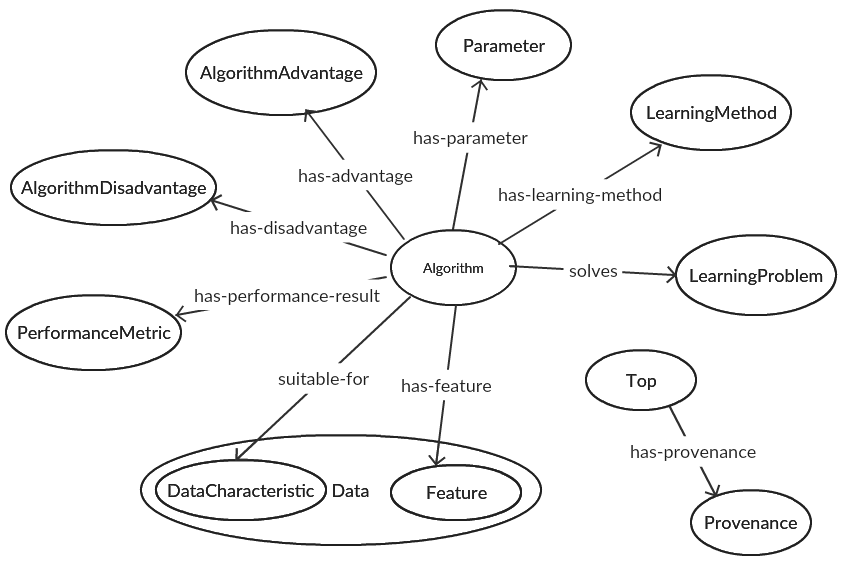
\includegraphics[width = 0.85 \linewidth]{img/ontologie_black.png}
        \caption{Vedere de ansamblu asupra ontologiei pentru machine learning: conceptul {\it Algorithm} 'si rolurile sale c'atre alte concepte.}
    \label{fig:onto}
\end{figure}

O vedere schematic'a asupra ontologiei apare 'in ~\ref{fig:onto}. 'In aceasta se pot observa rolurile care leag'a conceptul ML {\it Algorithm} de celelalte concepte din ontologie. Sunt expuse doar conceptele din primul nivel, excep'tie f'ac\i and clasa {\it Data} care este prezentat'a 'impreun'a cu cele dou'a subclase ale sale: {\it DataCharacteristic} 'si {\it Feature}. Imaginea eviden'tiaz'a datele con'tinute de ontologie: algoritmi, parametrii acestora, metode de 'inv'a'tare, problema de 'inv'a'tare pe care o rezolv'a, metrici de performan't'a, caracteristicile datelor 'si features, avantaje 'si dezavantaje, c\i at 'si informa'tii despre provenien'ta acestora.

\begin{figure}[h!]
    \centering
    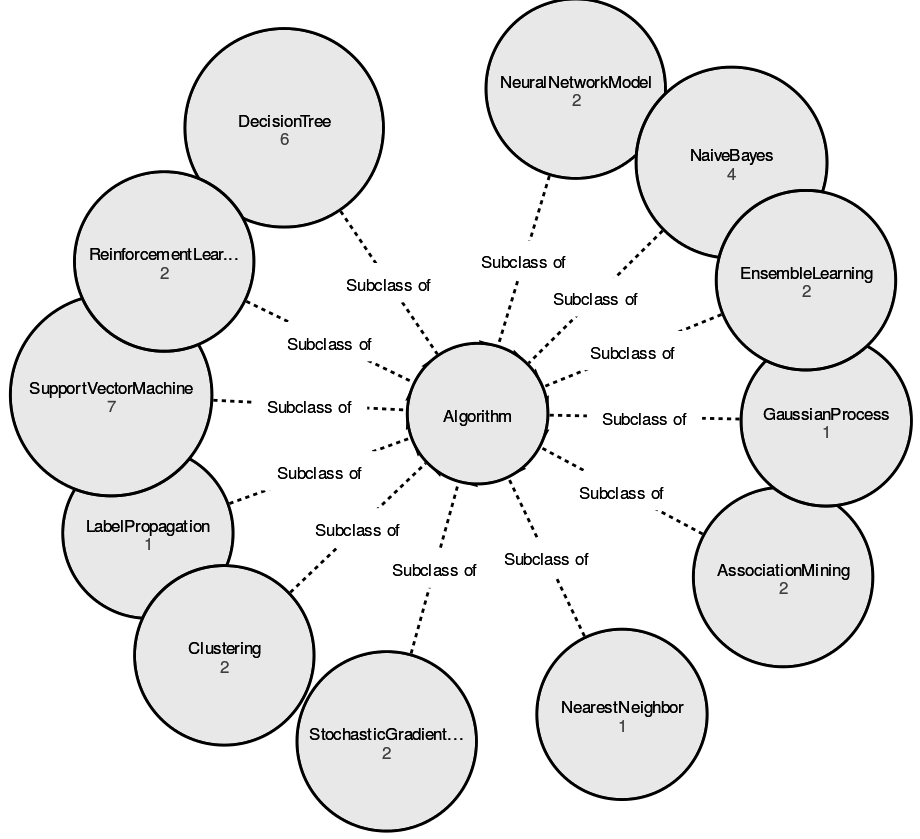
\includegraphics[width = 0.75 \linewidth]{img/algorithm_subclasses.png}
        \caption{Clasa {\it Algorithm}: diferiti algoritmi pentru ML}
    \label{fig:alg_sucls}
\end{figure}

Conceptul {\it Algorithm} este divizat 'in mai multe subconcepte care reprezint'a familii diferite de algoritmi, ce pot fi v'azute 'in Fig.~\ref{fig:alg_sucls}. Aduce 'impreun'a algoritmi care au metode de 'inv'a'tare supervizat'a, nesupervizat'a (cum ar fi clustering sau asociere), semi-supervizat'a 'si reinforcement. Cuprinde diferite varia'tii de algoritmi care sunt structura'ti 'in sublcase 'in func'tie de familia din care apar'tin: $DecisionTree$, $NeuralNetworkModel$, $NaiveBayes$, $SupportVectorMachine$, $LabelPropagation$ etc.

Similar conceptului de {\it Algorithm}, 'si parametrii sunt grupa'ti 'in clasa {\it Parameter} 'in func'tie de algoritmii c'arora le sunt asocia'ti. Figurile ~\ref{fig:subc_1} si ~\ref{fig:subc_2} ilustreaz'a acest fapt. Am ales divizarea parametrilor mai 'int\ia i 'in func'tie de familia de care apar'tin. Dac'a algoritmii din aceea'si familie nu folosesc aceia'si parametrii, am 'imp'ar'tit mai departe ace'sti parametrii 'in func'tie de indivizii c'arora le sunt asocia'ti. Parametrii compu'si apar'tin fiecare clasei c'areia 'ii descrie. 

\begin{figure}
    \centering
    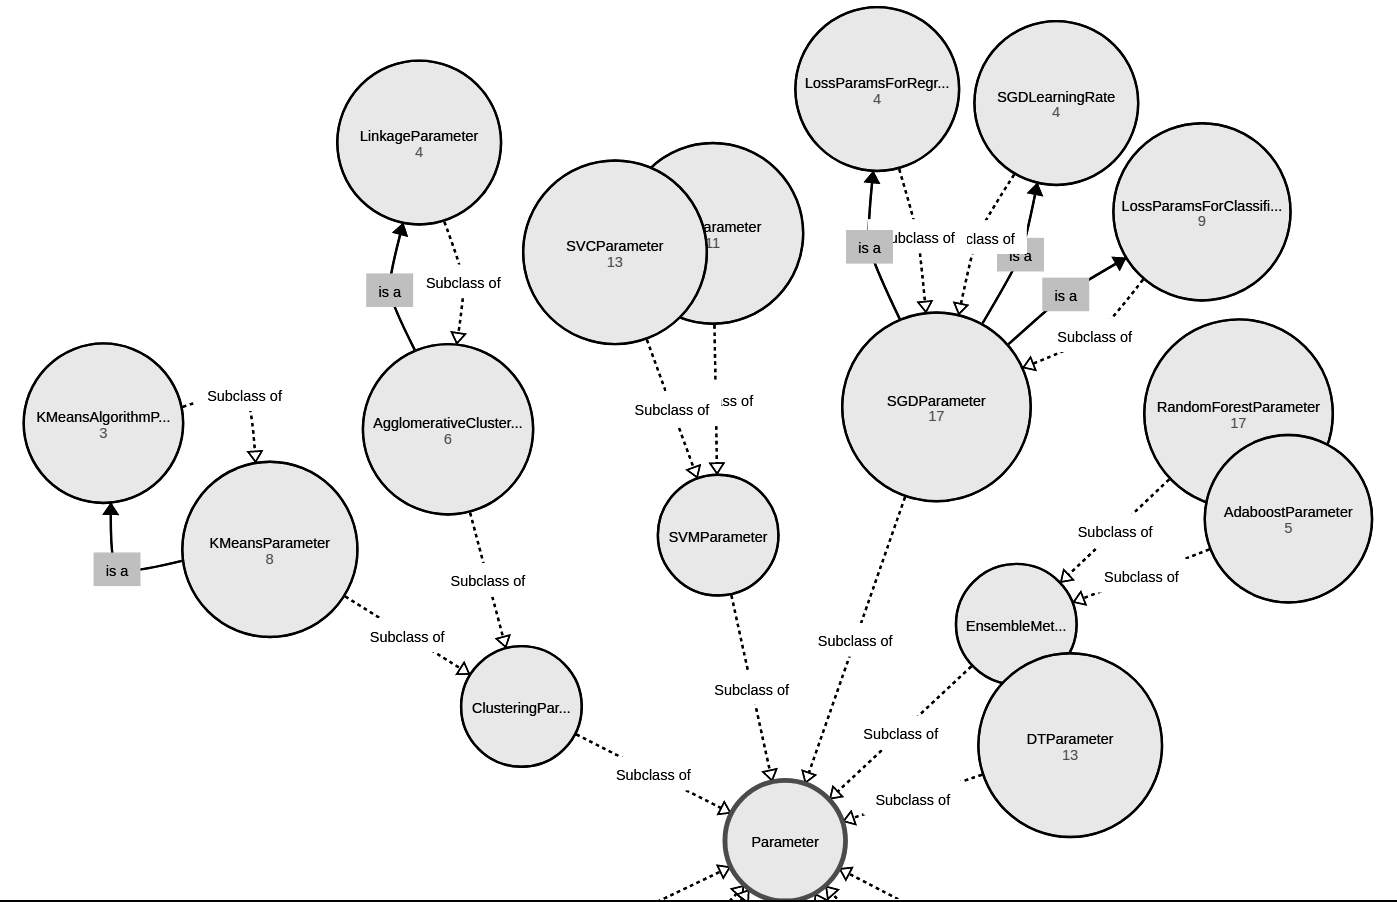
\includegraphics[width = 0.9 \linewidth]{img/properties_subcls_2.png}
        \caption{Prima parte a subconceptelor clasei $Parameter$}
    \label{fig:subc_1}
\end{figure}

\begin{figure}
    \centering
    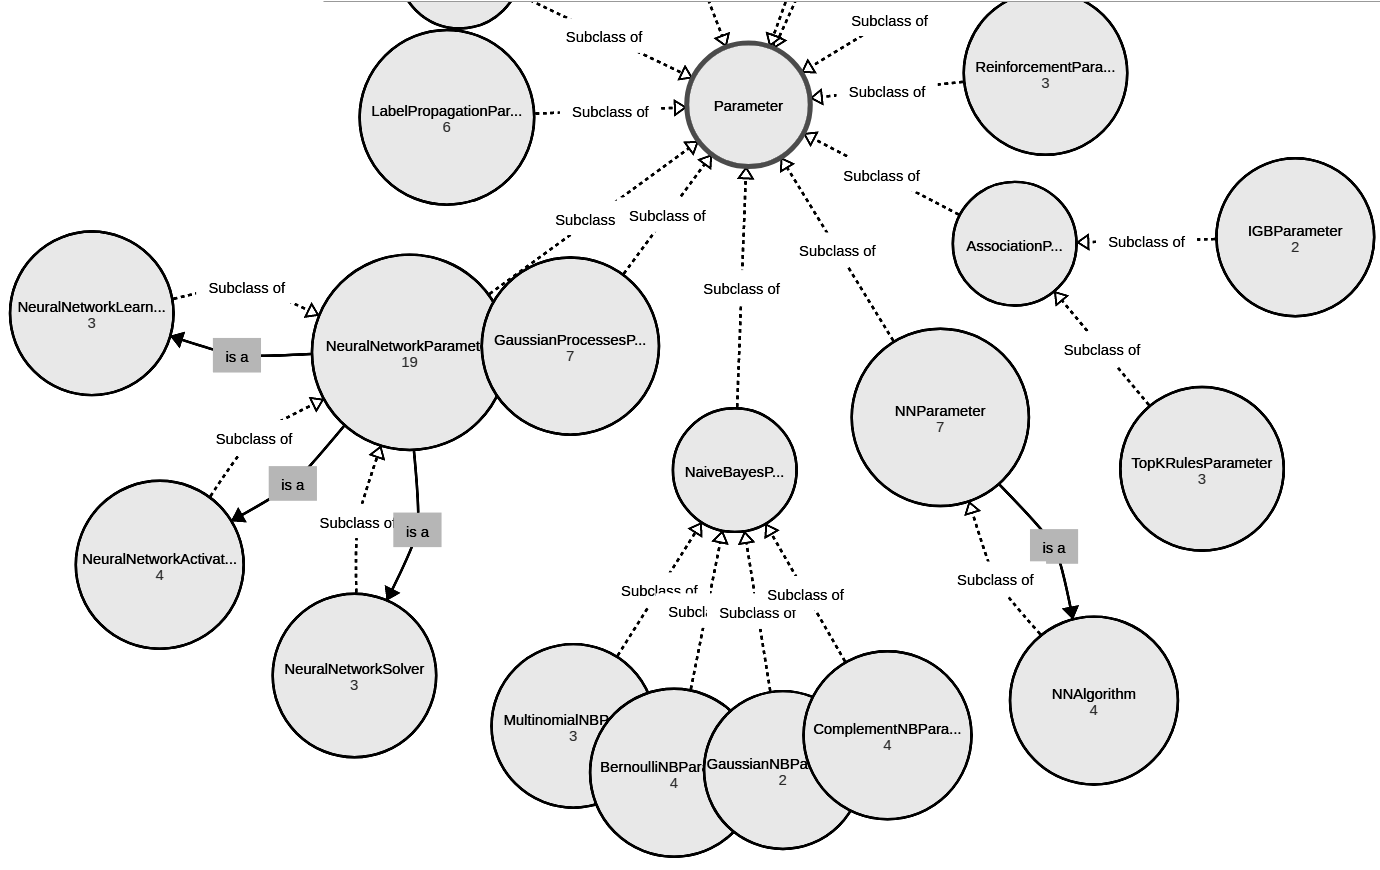
\includegraphics[width = 0.9 \linewidth]{img/properties_subcls_1.png}
        \caption{A doua parte a subconceptelor clasei $Parameter$}
    \label{fig:subc_2}
\end{figure}

Pentru popularea ontologiei ne-am bazat pe diferite tool-uri disponibile pentru ML. Pentru algoritmi pentru clustering, 'inv'a'tare semi-supervizat'a 'si superviza'ta, sursa principal'a de informa'tie este SciKit\footnote{https://scikit-learn.org/stable/}. Pentru association mining, am utilizat spmf\footnote{http://www.philippe-fournier-viger.com/spmf}. Datele despre reinforcement provin de la UNSW Sydney\footnote{https://www.cse.unsw.edu.au/~cs9417ml/RL1/algorithms.html}. 
%Being implemented taking into account good practices, our machine learning ontology can be further extended.


Ontologia a fost populat'a utiliz\ia nd Protege, acesta fiind o unealt'a automat'a pentru construirea ontologiilor. Permite ad'augarea conceptelor, a propriet'a'tilor 'si a indivizilor 'si genereaz'a un fi'sier 'in formatul dorit, OWL. Prezent'am in continuare exemple de implementare, fi'sierul complet fiind disponibil online\footnote{https://bitbucket.org/nicoleta\_corocea/ml\_chatbot/src/master/ontologies/machine-learning-ontology.owl}.

Proprietatea $has-learning-method$ prezint'a domeniul $Algorithm$ 'si codomeniul (range) $LearningMethod$ 'si este definit'a 'in secven'ta de cod~\ref{lst:proprOWL}.
\begin{lstlisting}[basicstyle=\footnotesize, caption = Proprietatea $has-learning-method$ 'in OWL, label=lst:proprOWL]

<owl:ObjectProperty rdf:about="http://www.semanticweb.org/
                                machine-learning-ontology/
                                has-learning-method">
    <rdfs:domain rdf:resource="http://www.semanticweb.org/
                                machine-learning-ontology
                                #Algorithm"/>
    <rdfs:range rdf:resource="http://www.semanticweb.org/
                                machine-learning-ontology
                                #LearningMethod"/>
</owl:ObjectProperty>
\end{lstlisting}


 Clasa $Algorithm$ din fi'sierul OWL este definit'a in secven'ta de cod~\ref{lst:proprClass}.
\begin{lstlisting}[basicstyle=\footnotesize,caption = Clasa $Algorithm$ 'in OWL, label=lst:proprClass]
    <owl:Class rdf:about="http://www.semanticweb.org
                        /machine-learning-ontology
                        #Algorithm"/>
 \end{lstlisting}   

O subclas'a a clasei $Algorithm$, $EnsembleMethod$, con'tine 'in defini'tia sa o leg'atur'a c'atre superclas'a si un comentariu:
\begin{lstlisting}[basicstyle=\footnotesize, caption = Clasa $Algorithm$ 'in OWL, label=lst:proprClass]
    <owl:Class rdf:about="http://www.semanticweb.org/machine-learning-ontology
                        #EnsembleLearning">
        <rdfs:subClassOf rdf:resource="http://www.semanticweb.org
                             /machine-learning-ontology #Algorithm"/>
        <rdfs:comment>
            The goal of ensemble methods is to combine the predictions
            of several base estimators built with a given learning algorithm in
            order to improve generalizability / robustness over a single estimator.
        </rdfs:comment>
    </owl:Class>
    
\end{lstlisting}
Individul $classification$ face parte din clasa $LearningProblem$ 'si este definit astfel: 

\begin{lstlisting}[basicstyle=\footnotesize]
    <owl:NamedIndividual rdf:about="http://www.semanticweb.org
                        /machine-learning-ontology#classification">
        <rdf:type rdf:resource="http://www.semanticweb.org
                        /machine-learning-ontology#LearningProblem"/>
    </owl:NamedIndividual>
    
\end{lstlisting}


'In tabelul ~\ref{table:individuals_table} prezent'am pentru un exemplu de algoritm, $decisionTreeClassifier$, propriet'a'tile 'si indivizii din codomeniul acestora. 

\begin{table}[ht]
\caption{Indivizi ai ontologiei}
\centering                          % tabel centrat 
\begin{tabular}{|c|c|c|c|}          % 4 coloane centrate 
\hline\hline                        % linie orizontala dubla
Proprietate& Indivizi & Clasa indivizilor \\ [0.5ex]   % inserare tabel
%heading
\hline                              % linie orizontal simpla
solves & classification & LearningProblem  \\               % corpul tabelului 
has-learning-method & supervised
& LearningMethod  \\[1ex]           % [1ex] adds vertical space
has-parameter &  \begin{tabular}{@{}c@{}} maxFeature, presort \\ max\_depth, class\_weight\end{tabular} & DTParameter \\[1ex]

suitable-for & nonLinearModels & DataCharacteristic \\[1ex]

has-feature-characteritic & complexInteractions & Feature \\[1ex]

has-advantage & whiteBox, handlesColinearity & AlgorithmAdvantage\\[1ex] 
has-disadvantage & proneToOutliers, proneToOverfitting & AlgorithmDisadvantage \\[1ex]

has-provenance & scikitSupervised & Provenance \\[1ex]

\hline                              
\end{tabular}
  % titlul tabelului
\label{table:individuals_table}                % \label{table:nonlin} introduce eticheta folosita pentru referirea tabelului in text; referirea in text se va face cu \ref{table:nonlin}
\end{table}

'In acest tabel am inserat numai o parte din propriet'a'tile algoritmului $decisionTree$, acestea fiind multe la num'ar. 'In acest fel, am detaliat 'in ontologie o mare majoritate a algoritmilor insera'ti. 


\section{Analiza arhitecturilor echivalente}

Arhitectura propus'a 'si implementat'a reprezint'a numai o solu'tie de rezolvare a problemei agentului explicativ 'in domeniul machine-learning. Are numeroase avantaje, cum ar fi: centralizarea tuturor apelurilor la un singur server, aspect de arhitectur'a pe niveluri 'si u'surin'ta de implementare. Un dezavantaj major al acesteia este acela c'a modulul $Reasoning\ Server$ fun'ctioneaz'a ca un intermediar 'intre $Tranlator$ 'si ontologie. 

'In figura ~\ref{fig:alternative_arh} se prezint'a o solu'tie alternativ'a care 'inl'atur'a dezavantajul men'tionat. Noua structur'a este modular'a 'si propune existen'ta a doua servere: $Reasoning\ Server$ 'si $Translator\ Server$.


\begin{figure}
    \centering
    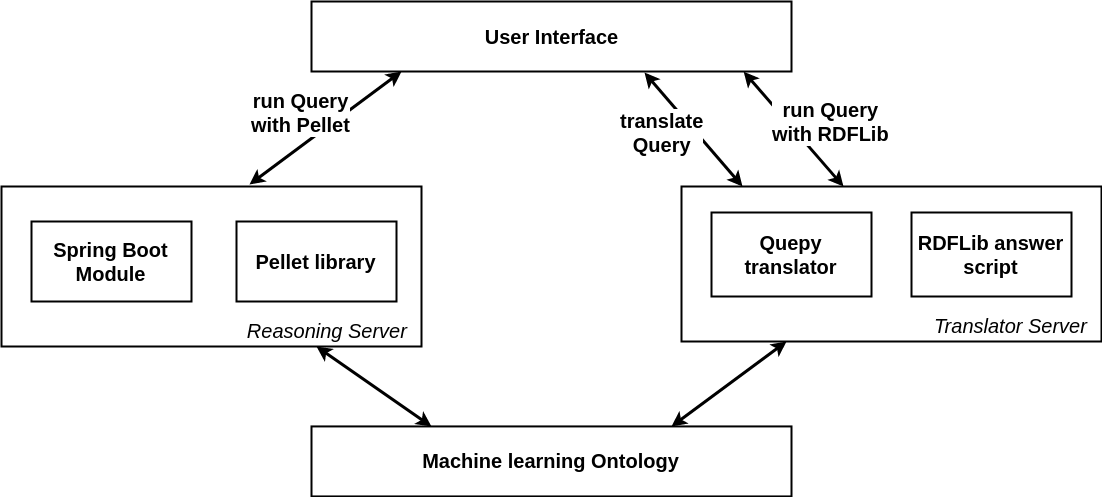
\includegraphics[width = 0.85 \linewidth]{img/arhitectura_alternativa.png}
        \caption{Arhitectur'a alternativ'a a aplica'tiei}
    \label{fig:alternative_arh}
\end{figure}

'In acest caz, $Reasoning\ Server$ va fi responsabil numai pentru request-urile care necesit'a utilizarea libr'ariei Pellet: interogarea ontologiei cu ajutorul Pellet, ob'tinerea claselor, a instan'telor 'si a propriet'a'tilor. $Translator\ Server$ devine responsabil pentru translatarea intreb'arilor din limbaj natural 'in limbaj de interogare SPARQL 'si pentru interogarea ontologiei folosind libr'aria RDFLib.

Arhitectura alternativ'a propus'a permite utilizarea modulului $Translator\ Service$ mult mai direct, f'ar'a 'int\ia rzieri. De'si pare o solu'tie mai potrivit'a pentru sistem, aceasta este dificil de implementat. Am 'incercat punerea 'in practic'a a acesteia 'inainte de varinta final'a din figura ~\ref{fig:arch}, dar am 'intampinat impedimente tehnice ale realiz'arii modulului $Translator$ sub form'a de server.



\section{Scenariu de utilizare}

'In figura ~\ref{fig:usecases} sunt prezentate func'tiile ce pot fi realizate din interfa't'a de c'atre utilizator. Acesta are posibilitatea de a scrie 'intrebarea, 'si, dup'a aceea, de a o translata 'in limbaj de interogare SPARQL. Utilizatorii mai avansa'ti pot edita interogarea SPARQL. Dup'a ace'sti pa'si, utilizatorul poate interoga ontologia utiliz'and Pellet sau RDFLib.  R'aspunsul acestor ac'tiuni poate fi vizualizat. 'In fereastra alternativ'a, utilizatorul poate solicita s'a vizualizeze toate clasele ontologiei, toate rolurile 'si to'ti indivizii.


\begin{figure}
    \centering
    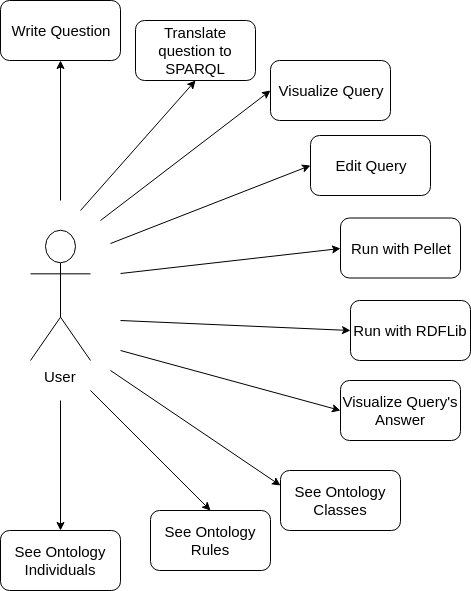
\includegraphics[width = 0.45 \linewidth]{img/use_case.png}
        \caption{Diagrama cazurilor de utilizare}
    \label{fig:usecases}
\end{figure}

'In continuare, vom ilustra capabilit'a'tile sistemului 'in cazurile de utilizare care con'tin 'intreb'ari complexe ce fac uz de 'imbun'at'a'tirile aduse la framework-ul Quepy. Acestea se rezum'a, pe scurt, la afi'sarea instan'telor 'in mod generalizat, afi'sarea algoritmilor care 'indeplinesc o condi'tie care con'tine operatorul $and$, $or$ 'si $not$.

Fie regulile $R_1$-$R_4$ care formalizeaz'a regulile de parsare ale 'intreb'arilor introduse. Semnifica'tia acestora este detaliat'a 'in tabelul ~\ref{tab:rules}.

\begin{table}[]
    \centering
    \begin{tabular}{|c|c|}
    \hline \hline
      Regul'a & Interpretare\\[0.5ex] \hline 
     $R_1$ & afi'seaz'a instan'tele clasei date \\[1ex]
  $R_2$ & algoritmi care rezolv'a problema precizat'a 'SI au metoda de 'inv'a'tare dat'a\\[1ex]
  $R_3$ & algoritmi potrivi'ti pentru o caracteristic'a a setului de date SAU o alt'a caracteristic'a\\[1ex]
  $R_4$ & algoritmi care NU au metoda de 'inv'a'tare cerut'a\\[1ex]
  \hline
    \end{tabular}
    \caption{Semnifica'tia regulilor date}
    \label{tab:rules}
\end{table}

Vom considera urm'atorul 'sir de 'intreb'ari introduse de utilizator, descrise de facilitatea pe care o 'indeplinesc:

\subsubsection{Afi'sarea indivizilor unui concept}
\begin{center}
{\it $Q_1$: Which are the instances of Algorithms?}
\end{center}

'Intrebarea poate fi formulat'a de asemenea ca {\it"individuals of Algorithm"},
       {\it "print Algorithm instances"},
       {\it "show Algorithms individuals"},
        {\it"list Algorithm"} 'si va fi interpretat'a 'si procesat'a 'in acela'si fel.
        
Cuv\ia ntul $individual$ poate fi 'inlocuit cu $instance$, dar poate de asemenea s'a 'si lipseasc'a. Dat fiind faptul c'a pluralul unui concept poate fi utilizat 'in mod obi'snuit, am considerat 'si acest caz.
Bazat pe regula Quepy $R_1$ (formalizat'a 'in sectiunea ~\ref{sec:parse}) interogarea SPARQL corespunz'atoare pentru $Q_1$ apare 'in Listing~\ref{lst:sparql:q1}.

%PREFIX owl:<http://www.w3.org/2002/07/owl#>
%PREFIX rdfs:<http://www.w3.org/2000/01/rdf-schema#>
\begin{figure}
\begin{footnotesize}
\begin{lstlisting}[captionpos=b, caption=Formalizarea SPARQL a interog'arii $Q_1$., label=lst:sparql:q1,
   basicstyle=\ttfamily,frame=single]
PREFIX rdf:<http://www.w3.org/1999/02/
           22-rdf-syntax-ns#>
PREFIX skos:<http://www.w3.org/2004/02/skos/core#>
PREFIX quepy:<http://www.machinalis.com/quepy#>
PREFIX ml:<http://www.semanticweb.org/
           machine-learning-ontology#>

SELECT DISTINCT ?x0 WHERE {
  ?x0 rdf:type ml:Algorithm.
}
\end{lstlisting}
\end{footnotesize}
\end{figure}

Folosind Pellet, r'aspunsul $a_1$ poate fi observat 'in listarea~\ref{lst:a1answ}, unde variabilae $?x0$ 'inlocuie'ste instan'tele conceptului {\it Algorithm}. 

\begin{center}
\begin{lstlisting}[basicstyle=\footnotesize, caption = R'aspunsul $a1$ la 'intrebarea $Q_1$, label=lst:a1answ]
{"head": { "vars": [ "x0" ]} ,
  "results": {
    "bindings": [
      {"x0":{"value":"gaussianProcessRegressor"}},
      {"x0":{"value":"oneClassSVM" }} 
      ...
      {"x0": {"value":"decisionTreeClassifier"}}]}}
\end{lstlisting}
\end{center}


R'aspunsul este ob'tinut pe baza urm'atoarelor axiome generale de incluziune 'in logic'a descriptiv'a:

\vspace*{0.3cm}
\begin{tabular}{ll}
1. & $GaussianProcess  \sqsubseteq Algorithm$\\
2. & $SupportVectorMachine  \sqsubseteq Algorithm$\\
3. & $DecisionTree  \sqsubseteq Algorithm$\\
4. & $gaussianProcessRegressor: GaussianProcess$\\
5. & $oneClassSVM: SupportVectorMachine$\\
6. & $decisionTreeClassifier: DecisionTree$\\
\end{tabular}
\vspace*{0.3cm}

Din axiomele (1) 'si (2) Pellet deduce c'a $GaussianProcess$, $DecisionTree$ 'si $Support$ $VectorMachine$ sunt subconcepte ale clasei $Algorithm$. Fiind date axiomele (4), (5) 'si (6), Pellet infer'a c'a $gaussianProcessRegressor$, $oneCLassSVM$ 'si $decisionTreeClassifier$ sunt de asemenea indivizi ai conceptului $Algorithm$. 

Diferit, utiliz\ia nd RDFLib, r'aspunsul este o lista goal'a deoarece RDFLib nu poate s'a ra'tioneze pe axiomele date 'si nu poate deduce c'a $gaussianProcessRegressor$, $oneCLassSVM$ 'si $decisionTreeClassifier$ sunt indivizi ai clasei $Algorithm$. 
'In acest caz, dac'a am fi dorit indivizii clasei $DecisionTree$ atunci RDFLib ar fi putut r'aspunde corect cu o list'a de indivizi.

De exemplu, fiind dat'a interogarea din secven'ta de cod~\ref{lst:sparql:dt} 'in care cerem instan'tele conceptului $DecisionTree$:


\begin{figure}[h]
\begin{footnotesize}
\begin{lstlisting}[captionpos=b, caption=Interogare SPARQL pentru ob'tinerea indivizilor clasei $DecisionTree$, label=lst:sparql:dt,
   basicstyle=\ttfamily,frame=single]
SELECT DISTINCT ?x0 WHERE {
  ?x0 rdf:type ml:DecisionTree.}
\end{lstlisting}
\end{footnotesize}
\end{figure}

R'aspunsul $a_2$ ob'tinut cu RDFLib poate fi v'azut 'in~\ref{lst:a2answ}.

\begin{center}
\begin{lstlisting}[basicstyle=\footnotesize,  caption = R'aspunsul $a2$, label=lst:a2answ]
    [
        { "x0": "decisionTreeRegressor"}, 
        ...
        {"x0": "decisionTreeClassifier"}, 
        {"x0": "id3"}
    ]
\end{lstlisting}
\end{center}

\subsubsection{Utilizarea operatorului AND}

{\it $Q_2$ algorithm that solves classification problem and has supervised learning method and has feature complexInteractions}

Poate fi scris'a 'si ca {\it "algorithm that solves classification and has supervised and complexInteractions" }. Regula Quepy $R_2$, conduce la interogarea SPARQL vizibil'a 'in secven'ta de cod~\ref{lst:sparqlq2}.
\begin{figure}[h]
\begin{footnotesize}
\begin{lstlisting}[captionpos=b, caption=Formalizarea SPARQL a interog'arii $Q_2$, label=lst:sparqlq2,  basicstyle=\ttfamily,frame=single]
SELECT DISTINCT ?x0 WHERE {
  ?x0 rdf:type ml:Algorithm.
  ?x0 ml:has-learning-method ?x1.
  ?x0 ml:solves ?x2.
  ?x0 ml:has-feature-characteristic ?x3.
  ?x1 rdf:type ml:LearningMethod.
  FILTER(?x1 = ml:supervised 
        && ?x2 = ml:classification 
        && ?x3 = ml:complexInteractions).
  ?x2 rdf:type ml:LearningProblem.
  ?x3 rdf:type ml:Feature.
}
\end{lstlisting}
\end{footnotesize}
\end{figure}

$?x0$ 'inlocuie'ste un individ al conceptului $Algorithm$. $?x1$ re'tine individul $supervised$ al conceptului $LearningMethod$, $?x2$ re'tine individul $classification$ al conceptului $LearningProblem$ 'si $?x3$ 'tine locul pentru individul $complexInteractions$ care este de tipul $Feature$.

R'aspunsul $a_3$ dat de Pellet este vizibil 'in listarea~\ref{lst:a3rsp}.
\newline
\begin{lstlisting}[basicstyle=\footnotesize, caption=R'aspunsul $a_3$ la 'intrebarea $Q_2$, label=lst:a3rsp]
{"x0": { "value": "decisionTreeClassifier" }}
\end{lstlisting}

Este ob'tinut pe baza urm'atorilor pa'si:

\vspace*{0.3cm}
\begin{small}
\begin{tabular}{ll}
7. & $DecisionTree  \sqsubseteq Algorithm$\\
8. & $decisionTreeClassifier:DecisionTree$\\
9. & $supervised: LearningMethod$\\
10. & $classification: LearningProblem$\\
11. & $complexInteractions: Feature$\\
12. & $(decisionTreeClassifier,supervised)$\\
    & $     : hasLearningMethod$\\
13. & $(decisionTreeClassifier,classification): solves$\\
14. & $(decisionTreeClassifier,complexInteractions)$: $hasFeatureCharacteristic$\\
\end{tabular}
\end{small}
\vspace*{0.3cm}

Aici, $decisionTreeClassifier$ este definit ca instan'ta a $Algorithm$. Bazat pe axiomele 12-14 este selectat ca rezultat corect de c'atre Pellet. Folosind RDFLib, r'aspunsul este o list'a goal'a deoarece  $decisionTreeClassifier$ nu este o instan't'a a conceptului $Algorithm$.

\subsubsection{Utilizarea operatorului OR}
{\it $Q_3$ Algorithms suitable for nonLinearModels or shortDocuments data characteristics}

Aceast'a 'intrebare poate fi scris'a ca {\it"algorithms suitable for nonLinearModels or shortDocuments"} 'si va conduce la acela'si rezultat. Interogarea este prezent'a 'in listarea~\ref{lst:sparqlq3}, ob'tinut'a pe baza $R_3$ (formalizat'a 'in tabelul ~\ref{tab:rules}).

\begin{figure}[h]
\begin{footnotesize}
\begin{lstlisting}[captionpos=b, caption=Formalizarea SPARQL a interog'arii $Q_3$, label=lst:sparqlq3,  basicstyle=\ttfamily,frame=single]
SELECT DISTINCT ?x0 WHERE {
 ?x0 rdf:type ml:Algorithm.
 ?x0 ml:suitable-for ?x1.
 ?x0 ml:suitable-for ?x2.
 ?x1 rdf:type ml:DataCharacteristic.
 FILTER(?x1 IN ( ml:nonLinearModels, ml:shortDocs)).
 ?x2 rdf:type ml:DataCharacteristic.}
\end{lstlisting}
\end{footnotesize}
\end{figure}


Variabila $?x0$ re'tine individul conceptului $Algorithm$. Variabila $?x1$ 'inlocuie'ste un individ din clasa $DataCharacteristic$ care este $nonLinearModels$ sau $shortDocs$. R'aspunsul $a_4$ dat de Pellet este~\ref{lst:rsp4}.

\begin{lstlisting}[basicstyle=\footnotesize, caption = R'aspunsul $a_4$ la 'intrebarea $Q_3$, label=lst:rsp4]
[
      {"x0": { "value": "mlpClassifier" }} ,
      {"x0": { "value": "mlpRegressor" }} ,
      {"x0": { "value": "decisionTreeClassifier" }} ,
      {"x0": { "value": "bernoulliNaiveBayes" }}
]
\end{lstlisting}

Vom prezenta axiomele pe baza c'arora $mlpClassifier$ 'si $bernoulliNaiveBayes$ sunt deduse ca r'aspunsuri corecte:

\vspace*{0.3cm}
\begin{small}
\begin{tabular}{ll}
15. & $NeuralNetworkModel  \sqsubseteq Algorithm$\\
16. & $NaiveBayes  \sqsubseteq Algorithm$\\
17. & $mlpClassifier:NeuralNetworkModel$\\
18. & $bernoulliNaiveBayes: NaiveBayes$\\
19. & $nonLinearModels: DataCharacteristic$\\
20. & $shortDocs: DataCharacteristic$\\
21. & $(mlpClassifier, nonLinearModels):suitable-for$\\
22. & $(bernoulliNaiveBayes, shortDocs):suitable-for$\\
\end{tabular}
\end{small}
\vspace*{0.3cm}

Indivizii da'ti pentru $DataCharacteristics$ sunt $nonLinearModels$ 'si $shortDocs$. Bazat pe cerere, instan'tele corespunz'atoare ale $Algorithm$ trebuie s'a satisfac'a proprietatea $suitable-for$. Pellet identific'a $mlpClassifier$ 'si $bernoulliNaiveBayes$ ca instan'te dorite ale $Algorithm$ bazat pe axiomele 15-18 'si 21-22. 
RDFLib nu poate afla r'aspusnul corect deoarece nu poate ra'tiona.
%%%%%%%%%%%%%%%%%%%%%%%%%%%%%%%%%%%%%%%%%%%%%%%%%%%%%%%%%%%%%%%%%%%%%%%%%%%%%
\subsubsection{Utilizarea operatorului MINUS}
{\it $Q_4$ algorithms that do not have supervised learning method}

Dac'a aceast'a interogare se scrie ca {\it"algorithm that does not have supervised"} se va ob'tine acela'si rezultat. $R_4$ (formalizat'a in tabelul ~\ref{tab:rules}) este regula de identificare Quepy pentru urm'atoarea expresie SPARQL din secven'ta de cod~\ref{lst:sparqlq4}.

\begin{figure}[h]
\begin{footnotesize}
\begin{lstlisting}[captionpos=b, caption=Q4 SPARQL query, label=lst:sparqlq4,  basicstyle=\ttfamily,frame=single]
SELECT DISTINCT ?x0 WHERE {
  ?x0 rdf:type ml:Algorithm.
  MINUS { ?x0  ml:has-learning-method ?x1.   FILTER(?x1 = ml:supervised).}.
  ?x1 rdf:type  ml:LearningMethod.
}
\end{lstlisting}
\end{footnotesize}
\end{figure}
%\vspace{-0.5em}
Variabila $?x0$ re'tine indivizii conceptului $Algorithm$. Variabila $?x1$ 'inlocuie'ste $supervised$ care are tipul $LearningMethod$. $?x0$ nu trebuie s'a aib'a metoda de 'inv'a'tare $?x1$.

R'aspunsul dat de Pellet este $a_5$, ce poate fi observt 'in secven'ta de cod~\ref{lst:rspa5}.

\begin{lstlisting}[basicstyle=\footnotesize, caption=R'aspunsul $a_5$ la 'intrebarea $Q_4$, label=lst:rspa5]
[
    {"x0": { "value": "oneClassSVM" }} ,
     ...
    {"x0": { "value": "labelPropagation" } }
 ]
\end{lstlisting}

Axiomele utilizate pentru $labelPropagation$ sunt:

\vspace*{0.3cm}
\begin{small}
\begin{tabular}{ll}
23. & $LabelPropagation  \sqsubseteq Algorithm$\\
24. & $labelPropagation:LabelPropagation$\\
25. & $supervised: LearningMethod$\\
26. & $semiSuperviseds: LearningMethod$\\
27. & $(labelPropagation, semiSupervised)$: $has-learning-method$\\
\end{tabular}
\end{small}
\vspace*{0.3cm}

Individul $labelPropagation$ este de tipul $LabelPropagation$ 'si, fiind date axiomele 23-24, este de tip $Algorithm$ automat. Prin interogarea SPARQL curent'a, dorim ca instan'tele clasei $Algorithm$ care nu au metoda de 'inv'a'tare $supervised$. Cu ajutorul axiomelor 26-27, $labelPropagation$ este definit ca r'aspunsul corect pentru metoda de 'inv'a'tare $semiSupervised$.
Datorit'a faptului c'a RDFLib nu poate infera axioma precum 23, nu poate da un r'aspuns.

%%%%%%%%%%%%%%%%%%%%%%%%%%%%%%%%%%%%%%%%%%%%%%%%%%%%%%%%%%%%%%%%%%%%%%%%%%%
\chapter{Testare 'si Validare}\label{sec:testing}

\section{Testare}
'In cadrul test'arii am verificat fiecare punct terminal pentru a analiza cum se comport'a 'in cazuri specifice de utilizare, c\ia t 'si 'in momentele 'in care sunt introduse date incorecte.

Testele au fost realizate 'tin\ia nd cont de separarea opera'tiilor pe care le pot face utilizatorii din interfa't'a.

\subsubsection{Testarea func'tion'arii translat'arii din limbaj natural 'in SPARQL}

Utilizeaz'a punctul terminal $/translateQuery$. 

Pentru analiza cazului corect de func'tionare, consider'am 'intrebarea de test:
\begin{center}
$T_{11}\ :\ List\ DecisionTree\ individuals$.
\end{center}

Ac'tion\ia nd butonul pentru translatare, r'aspunsul ob'tinut este prezent 'in secven'ta de cod~\ref{lst:test11}:

\begin{figure}[h]
\begin{footnotesize}
\begin{lstlisting}[captionpos=b, caption=R'aspuns SPARQL pentru T_{11}, label=lst:test11,  basicstyle=\ttfamily,frame=single]
PREFIX owl: <http://www.w3.org/2002/07/owl#>
PREFIX rdfs: <http://www.w3.org/2000/01/rdf-schema#>
PREFIX rdf: <http://www.w3.org/1999/02/22-rdf-syntax-ns#>
PREFIX skos: <http://www.w3.org/2004/02/skos/core#>
PREFIX quepy: <http://www.machinalis.com/quepy#>
PREFIX ml: <http://www.semanticweb.org/machine-learning-ontology#>

SELECT DISTINCT ?x0 WHERE {
  ?x0 rdf:type ml:DecisionTree.
}
\end{lstlisting}
\end{footnotesize}
\end{figure}

Pentru analiza comportamentului 'in cazul 'in care nu se introduce o intrebare valid'a, consider'am:
\begin{center}
$T_{12}\ :\ TEST\ 12$.
\end{center}

R'aspunsul primit este o avertizare: {\it Could not translate question to SPARQL query!}

'In ambele cazuri, sistemul s-a comportat a'sa cum era de a'steptat.

\subsubsection{Testarea func'tion'arii interog'arilor utiliz\ia nd Pellet}

Interogarea ontologiei folosind Pellet utilizeaz'a punctul terminal $/runQueryWithPellet$.
O intrare valid'a pentru acest caz este interogarea afisat'a 'in ~\ref{lst:test11}. Raspunsul ob'tinut pentru aceast'a interogare este observabil 'in secven'ta de cod~\ref{lst:correctansw11}:
\begin{lstlisting}[basicstyle=\footnotesize, caption = R'aspuns la 'intrebarea $T_{11} prin Pellet$, label=lst:correctansw11]
[
    {"x0": { "value": "c5dot0" }} ,
    {"x0": { "value": "cart" }} ,
    {"x0": { "value": "c4dot5" }} ,
    {"x0": { "value": "id3" }} ,
    { "x0": { "value": "decisionTreeRegressor" }} ,
    {"x0": { "value": "decisionTreeClassifier" }}
]
\end{lstlisting}

Pentru o interogare goal'a cum ar fi o interogare care con'tine numai spa'tii, r'aspunsul const'a intr-un avertisment:  {\it This is not a valid SPARQL query!}.

Pentru o interogare cu erori de sintax'a sau din care lipse'ste prefixul, cum ar fi secven'ta de cod~\ref{lst:test2}:

\begin{figure}[h]
\begin{footnotesize}
\begin{lstlisting}[captionpos=b, caption=Interogare SPARQL defectuoas'a, label=lst:test2,  basicstyle=\ttfamily,frame=single]
SELECT DISTINCT ?x0 WHERE {
  ?x0 rdf:type ml:DecisionTree.
}
\end{lstlisting}
\end{footnotesize}
\end{figure}


R'aspunsul ob'tinut este avertismentul din cazul precedent:  {\it This is not a valid SPARQL query!}.

'In cazul 'in care se cer instan'tele unei clase DecisionTree\_TEST inexistente, atunci sistemul semnaleaz'a o avertizare: {\it Undefined class used in query: DecisionTree\_TEST}.


\subsubsection{Testarea func'tion'arii interog'arilor folosind RDFLib}


Interogarea ontologiei folosind RDFLib utilizeaz'a punctul terminal $/runQueryWithRDFLib$.
secven'ta de cod~\ref{lst:test11} reprezint'a o intrare valid'a pentru acest caz. Raspunsul ob'tinut pentru aceast'a interogare este observabil 'in secven'ta de cod~\ref{lst:correctansw11rdf}:
\begin{lstlisting}[basicstyle=\footnotesize,  caption = R'aspuns la 'intrebarea $T_{11} prin RDFLib$, label=lst:correctansw11rdf]
[
    { "x0": "c5dot0"}, 
    {"x0": "decisionTreeRegressor"}, 
    {"x0": "c4dot5" }, 
    {"x0": "cart"}, 
    {"x0": "decisionTreeClassifier"}, 
    {"x0": "id3"}
]

\end{lstlisting}

Pentru o interogare goal'a cum ar fi o interogare care con'tine numai spa'tii, r'aspunsul const'a intr-un avertisment:  {\it  Something went wrong and your query could not be processed!}.

Pentru o interogare cu erori de sintax'a sau din care lipse'ste prefixul, cum ar fi secven'ta de cod~\ref{lst:test2}, r'aspunsul ob'tinut este avertismentul din cazul precedent:  {\it Something went wrong and your query could not be processed!}.

'In cazul 'in care se cer instan'tele unei clase DecisionTree\_TEST inexistente, atunci sistemul nu poate identifica gre'seala 'si va returna o list'a goal'a.

\subsubsection{Testarea func'tion'arii solicit'arii claselor, rolurilor 'si instan'telor ontologiei}
Pentru a ob'tine clasele, rolurile 'si instan'tele ontologiei utilizatorul nu trebuie s'a introduc'a inputuri. Astfel, nu exist'a cazuri 'in care acestea pot func'tiona gre'sit.

Solicitarea claselor ontologiei prina c'tionarea butonului specific va returna o list'a complet'a cu conceptele acesteia.

Cererea rolurilor din ontologie va returna o list'a cu aceste roluri, incluz\ia nd $bottom$ $ObjectProperty$ 'si $topObjectProperty$.

La solicitarea tuturor instan'telor din ontologie se returneaz'a o list'a care le con'tine, f'ar'a alte ad'augiri.

%%%%%%%%%%%%===========================
\section{Performan't'a}

Am evaluat aplica'tia utiliz\ia nd un set de 10 'intreb'ari pe care le-am rulat de 100 de ori. Am calculat media ob'tinerii unei interog'ari SPARQL 'si um'arul de constr'angeri pe care 'il are aceasta, num'arul de indivizi din r'aspunsul dat de Pellet 'si timpul afl'arii acestui r'aspuns, num'arul de instan'te con'tinute de r'aspunsul dat de RDFLib 'si timpul 'in care acesta a fost ob'tinut. Am utilizat 'intreb'arile din tabelul~\ref{tab:perfintr}, unde $TQ$ refer'a o 'intrebare de test (test question).

\begin{table}[]
    \centering
\begin{tabular}{ll}
$TQ_1$ & list Algorithm individuals\\
$TQ_2$ & list DecisionTree individuals\\
$TQ_3$ & sarsa learning methods\\
$TQ_4$ & What are the advantages of kMeans?\\
$TQ_5$ & show details of identity\\
$TQ_6$ & Data subclass\\
$TQ_7$ & class of mlpRegressor\\
$TQ_8$ & algorithm that solves classification problem and has\\
 & supervised learning method and has feature \\
 & complexInteractions \\
$TQ_9$ & algorithms that do not have supervised learning  \\
& method \\
$TQ_{10}$ & algorithm suitable for nonLinearModels \\
& or shortDocuments\\
\end{tabular}
    \caption{Lista 'intreb'arilor utilizate pentru evaluarea performan'tei}
    \label{tab:perfintr}
\end{table}




'In tabelul ~\ref{table:performance} pot fi observate rezultatele acestei analize. Datorit'a arhitecturii sistemului, timpul ob'tinerii r'aspunsurilor de la modulul $Translator$ este 'int\ia rziat cu aproximativ 1 secunda. 'In schimb, libr'aria Pellet extrage r'aspunsul 'intr-un timp foarte bun. 'In documenta'tia oficial'a \cite{SirinPellet:Reasoner}, E. Sirin aminte'ste 'in sec'tiunea 7 c'a performan'ta ra'tionatorului Pellet nu depinde de dimnesiunea num'arului de date, rezultat pe care l-am ob'tinut 'si noi.
\begin{table}
\caption{Performan'ta sistemului}
\centering            
% tabel centrat |p{1cm}|p{3cm}|p{2cm}|p{2cm}|p{2cm}|p{1cm}|p{1cm}|
\resizebox{\linewidth}{!}{
\begin{tabular}{|c|c|c|c|c|c|c|}          % 4 coloane centrate 
\hline\hline                        % linie orizontala dubla
TQ &  Constr\ia ngeri  & Quepy  & Nr. de rezultate & Pellet  & Nr. de rezultate  & RDFLib \\ [0.5ex]   % inserare tabel
& SPARQL & time(ms) & Pellet & Time(ms) & RDFLib & time(ms)\\ [0.5ex]
%heading
\hline                              % linie orizontal simpla
$TQ_1$ & 1 & 1930 & 32 & 7  & 0 & 1902 \\[1ex]
$TQ_2$ & 1 & 1719 & 6  & 5 & 6 & 1691 \\[1ex]
$TQ_3$ & 3 & 1852 & 1  & 5 & 0 & 1782 \\[1ex]
$TQ_4$ & 3 & 1828 & 3  & 5 & 0 & 1899 \\[1ex]
$TQ_5$ & 3 & 1715 & 1  & 4 & 1 & 1657 \\[1ex]
$TQ_6$ & 2 & 1867 & 4  & 6 & 2 & 1672 \\[1ex]
$TQ_7$ & 2 & 1723 & 3  & 6 & 2 & 1667 \\[1ex]
$TQ_8$ & 8 & 1915 & 1  & 11 & 0 & 1786 \\[1ex]
$TQ_9$ & 3 & 1830 & 13  & 4 & 0 & 1774 \\[1ex]
$TQ_10$ & 6 & 2057 & 4 & 8 & 0 & 2083 \\[1ex]

\hline                              
\end{tabular}
}
  % titlul tabelului
\label{table:performance}                % \label{table:nonlin} introduce eticheta folosita pentru referirea tabelului in text; referirea in text se va face cu \ref{table:nonlin}
\end{table}
'In urma unei analize mai profunde 'si separate a $Translatorului$ am ob'tinut rezultatele din tabelul ~\ref{table:performance_tr}. 
\begin{table}
\caption{Performan'ta modulului $Translator$}
\centering                          % tabel centrat 
\begin{tabular}{|c|c|c|c|c|}          % 4 coloane centrate 
\hline                    % linie orizontala dubla
TQ &  Constr\ia ngeri  & Quepy  & Nr. de rezultate  & RDFLib \\ [0.5ex]   % inserare tabel
& SPARQL & time(ms)  & RDFLib & time(ms)\\ [0.5ex]
%heading
\hline  \hline                            % linie orizontal simpla
$TQ_1$ & 1 & 23  & 0 & 23 \\[1ex]
$TQ_2$ & 1 & 3 & 6 & 8 \\[1ex]
$TQ_3$ & 3 & 2 & 0 & 19 \\[1ex]
$TQ_4$ & 3 & 1  & 0 & 19 \\[1ex]
$TQ_5$ & 3 & 3  & 1 & 19 \\[1ex]
$TQ_6$ & 2 & 3  & 2 & 17 \\[1ex]
$TQ_7$ & 2 & 3  & 2 & 17 \\[1ex]
$TQ_8$ & 8 & 5  & 0 & 41 \\[1ex]
$TQ_9$ & 3 & 4  & 0 & 24 \\[1ex]
$TQ_10$ & 6 & 2 & 0 & 32 \\[1ex]

\hline                              
\end{tabular}
  % titlul tabelului
\label{table:performance_tr}                % \label{table:nonlin} introduce eticheta folosita pentru referirea tabelului in text; referirea in text se va face cu \ref{table:nonlin}
\end{table}


Acestea de confirm'a faptul c'a transmisia datelor dintre $Translator$ 'si $Reasoning$ $Service$ dureaz'a mult, dar ne arat'a 'sii o leg'atur'a 'intre numarul de rezultate ob'tinute de RDFLib 'si timpul de execu'tie pentru ob'tinerea acestora. Se poate observa c'a timpul scade odat'a cu cre'sterea num'arului de rezultate.



%%%%%%%%%%%%%%%%%%%%%%%%%%%%%%%%%%%%%%%%%%%%%%%%%%%%%%%%%%%%%%%%%%%%%%%%%%%
\chapter{Manual de Instalare 'si Utilizare}
\label{sec:instalare}

Capitolul de fa't'a cuprinde 'in prima parte instruc'tiuni pentru instalarea sistemului 'si aducerea 'in starea de rulare. A doua parte con'tine un manual de utilizare destinat utilizatorilor, pentru a cunoa'ste modalitatea de folosire a sistemului

\section{Instalarea sistemului}

Instalarea sistemului presupune trei pa'si prin care se va ob'tine sistemul activ, gata pentru a fi utilizat de clien'ti. Necesit'a un set de prerechizite, iar apoi const'a 'in pornirea serverului 'si a interfe'tei utilizator. Sistemul este disponibil 'intr-un repository de git\footnote{https://bitbucket.org/nicoleta_corocea/ml_chatbot/src/master/}. Ace'sti pa'si sunt descri'si 'in continuare:

\begin{itemize}
    \item Primul pas const'a 'in asigurarea c'a uneltele necesare utiliz'arii aplica'tiei sunt instalate pe sistemul de dezvoltare. Aplica'tia este construit'a din trei module separate ce au nevoie, fiecare de o libr'arie instalat'a pe sistem pentru a func'tiona. Interfa'ta a fost dezvoltat'a 'in Angular 'si necesit'a versiunea 11.13.0 de NodeJS sau mai mare. Serverul pentru ra'tionare este dezvoltat 'in Java 10.0.3, dar versiunea poate s'a difere, c'at timp este mai mare de 8. Pentru func'tionarea corespunz'atoare a modulului pentru translatarea din limbaj natural 'in limbaj de interogare SPARQL este necesar'a versiunea 2.17.15 de Python. De asemenea, trebuie s'a existe suport pentru framework-ul Quepy. Pentru acesta, trebuie urm'arit tutorialul\footnote{Quepy installation https://quepy.readthedocs.io/en/latest/installation.html}.
    \item Al doilea pas const'a 'in pornirea serverului. Acesta a fost dezvoltat cu ajutorul mediului de dezvoltare IntelliJ. Pentru pornirea serverului, se va deschide proiectul cu IntelliJ sau cu orice alt mediu de dezvoltare specific. Se acceseaz'a $ChatbotApplication$ 'si se ruleaz'a ca aplica'tie Spring Boot. 'In lipsa unui IDE, se va identifica fi'sierul .jar al proiectului 'si se va rula cu comanda {\it java\ -jar\ target/chatbot-<version>-SNAPSHOT.jar}. Pentru succesul 'in rularea serverului, trebuie ca portul 8080 s'a fie disponibil.
    \item Pentru pornirea interfe'tei utilizator, se deschide o instan'ta de Intellij cu proiectul interfe'tei. Este necesar s'a se ruleze ca $Angular\ CLI\ Server$. 
\end{itemize}

Odat'a parcur'si ace'sti pa'si, sistemul este disponibil 'in browser la adresa $http://localhost:4200/$. Pentru cazul 'in care aplica'tia va fi disponibil'a pe un server public, utilizatorii vor avea nevoie s'a acceseze numai interfa'ta utilizator prin adresa pus'a la dispozi'tie de acel provider.

\section{Manual de utilizare}

Agentul explicativ pentru 'inv'a'tarea automat'a a fost dezvoltat pentru ca utilizatorii s'a in'teleag'a conceptele de baz'a ale func'tion'arii domeniului. Sistemul st'a la dispozi'tia utilizatorului pentru a r'aspunde la 'intreb'arile adresate 'in limbaj natural. Pentru utilizarea sistemului, utilizatorii trebuie s'a dispun'a de un browser web. 

\begin{figure}
    \centering
    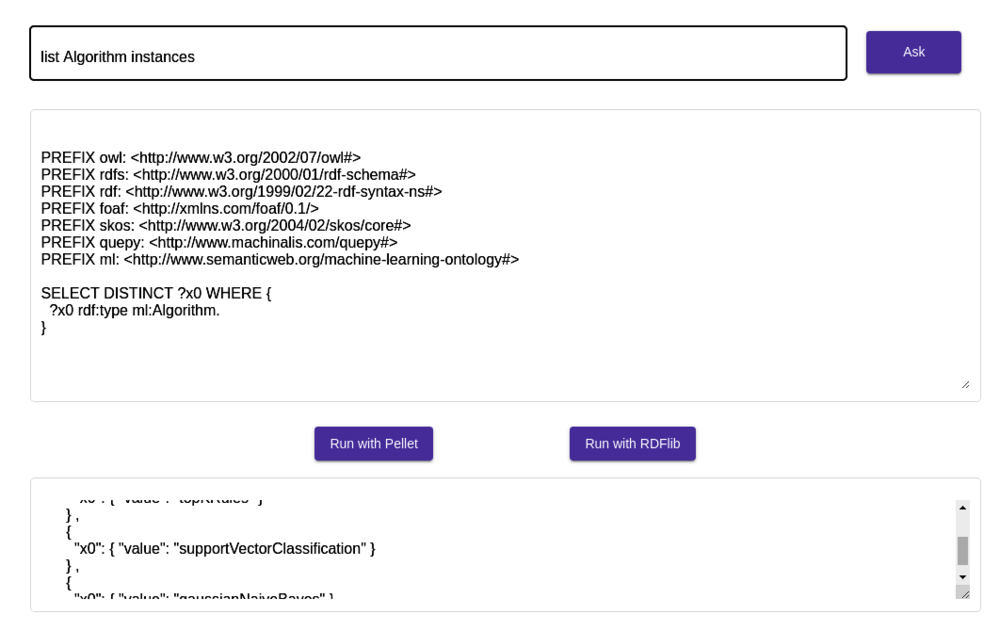
\includegraphics[width = 0.65 \linewidth]{img/pg1_cut.png}
        \caption{Pagina pentru adresarea 'intreb'arilor}
    \label{fig:ui1}
\end{figure}

Utilizarea paginii pentru ob'tinerea r'aspunsurilor prin limbaj natural ce poate fi observat'a 'in figura ~\ref{fig:ui1} se face prin urm'atorii pa'si:
\begin{itemize}
    \item Utilizatorul va accesa tab-ul denumit $Ask\ a\ question$.
    \item Introducerea 'intreb'arii 'si ac'tionarea butonului $Ask$. 'Intreb'arile trebuie s'a fie din lista propus'a din Anexa B. 
    \item Vizualizarea sau modificarea interog'arii SPARQL din caseta destinat'a. Utilizatorii pot vizualiza interogarea, iar cei mai experimenta'tii o pot modifica 'tin\ia nd cont de regulile de scriere ale interog'arilor SPARQL.
    \item Ac'tionarea interog'arii cu Pellet sau RDFLib 'si vizionarea rezultatului. Utilizatorul are la dispozi'tie dou'a butoane $RunWithPellet$ 'si $RunWithRDFLib$ pe care le paote ac'tiona.
\end{itemize}

Sistemul pune la dispozi'tie 'si o pagin'a 'in care utilizatorul poate vedea ce elemente de'tine ontologia, observat'a 'in figura ~\ref{fig:ui2}. Pentru utilizarea acestei pagini, clientul va accesa tab-ul $Ontology\ Details$. 'In aceast'a fereastr'a, va ac'tiona butonul $Individuals$ pentru a ob'tine o list'a cu to'ti indivizii ontologiei. Butonul $Classes$ determin'a afi'sarea unei liste cu conceptele ontologiei, iar butonul $Properties$ va afis'a toate propriet'a'tile ontologiei.


\begin{figure}
    \centering
    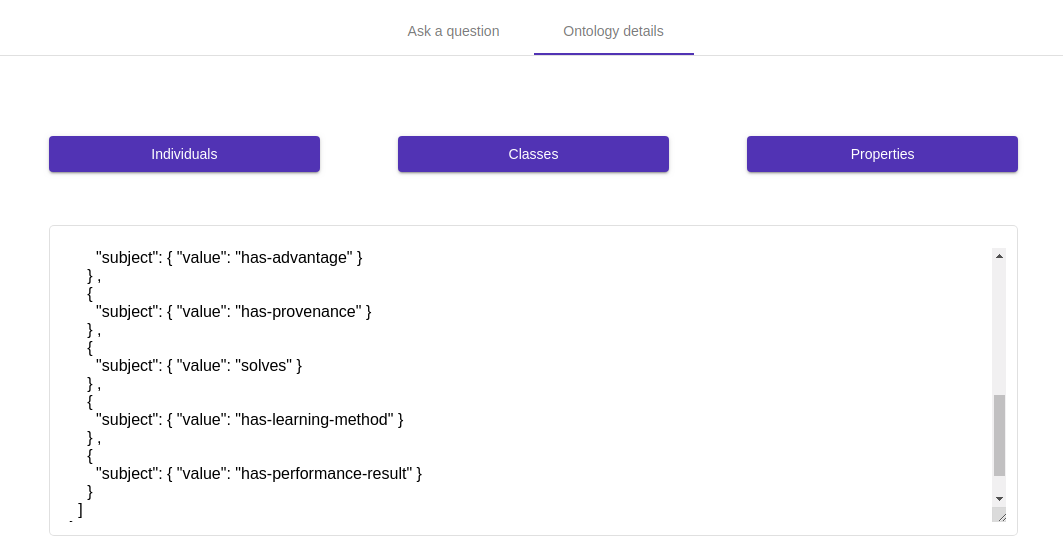
\includegraphics[width = 0.65 \linewidth]{img/ui2.png}
        \caption{Pagina pentru explorarea ontologiei}
    \label{fig:ui2}
\end{figure}

%%%%%%%%%%%%%%%%%%%%%%%%%%%%%%%%%%%%%%%%%%%%%%%%%%%%%%%%%%%%%%%%%%%%%%%%%%
\chapter{Concluzii}
\label{sec:concluzii}

'In prima parte a acestui capitol se prezint'a o retrospectiv'a asupra sistemului, pun'and 'in valoare modul de r'aspuns la 'intreb'arile adresate 'in limbaj natural. O analiz'a a dezvolt'arilor ulterioare ce pot 'imbun'at'a'ti sistemul de r'aspuns vor fi prezentate 'in partea a doua a acestui capitol.

\section{Contribu'tii 'si realiz'ari}
Agentul cu rol 'in explicarea 'inv'at'arii automate are la baz'a o ontologie ce poate fi interogat'a prin intermediul 'intreb'arilor 'in limbaj natural translatate 'in SPARQL. Acesta dore'ste acomodarea utilizatorului cu domeniul 'inv'a't'arii automate pentru a diminua ne'increderea 'si scepticismul 'in sistemele automate. 'In dezvoltarea acestui proiect am contribuit cu:

\begin{itemize}
    \item {\it Dezvoltarea\ unei\ arhitecturi\ ce\ integreaz'a\ explicarea\  'in\ sistemele\ de\ r'aspundere\ la\ 'intrebari} -  Arhitectura propus'a este distribuit'a 'in microservicii, fiecare component'a a sa fiind responsabil'a de executarea unei fun'ctionalit'ati. Aceast'a arhitectur'a se prezint'a ca o arhitectur'a pe nivele, avantajul ei fiind c'a modulele sunt independente 'si pot fi 'intre'tinute cu u'surin't'a. Dat'a fiind nevoia de explicare a procesului de ob'tinere a unui r'aspuns, c\ia t 'si de a m'ari transparen'ta 'in aplica'tie, arhitectura este adaptat'a pentru a face fa't'a acestor cerin'te. Utilizatorul este implicat 'in procesul de extragere a r'aspsunsului, fiind con'stient de pa'sii necesari. Ontologia 'isi expune elementele pentru ca utilizatorul s'a 'in'teleag'a provenien't'a r'aspunsului.

    
    \item {\it Transformarea\ libr'ariei\ Pellet\ pentru\ a\ func'tiona\ ca\ server} - Datorit'a necesit'a'tii de a avea un sistem care 'i'si expune func'tionalit'a'tile online, dat fiind vasta r'asp'andire a aplica'tiilor web, am integrat un modul Spring Boot 'in libr'aria Pellet. Aceast'a strategie are ca principal avantaj men'tinerea modularit'a'tii bazat'a pe limbaj 'si func'tionalit'a'ti. Un alt avantaj major este capabilitatea de expunere a func'tionalit'a'tilor ra'tionatorului Pellet ca endpoint-uri. Acest lucru reprezint'a o facilitate general'a, ce poate fi folosit'a  
  
    \item {\it Extinderea\ framework-ului\ Quepy\ pentru\ a\ permite\ opera'tii\ cu\ operatori\ logici} - Pentru a acoperi nevoia translat'arii din limbaj natural 'in limbaj de interogare SPARQL am implementat un proiect Quepy. Acesta cuprinde o abstractizare a elementelor ontologiei, dar 'si reguli de parsare 'si identificare a 'intreb'arilor care sunt posibile a fi puse. 'Intreb'arile au fost selectate 'si dezvoltate pentru a cuprinde 'si cerin'te mai complexe, c'at 'si probleme des 'int\ia lnite pe forumuri. La acest mod de procesare a limbajului ntural, am extins framework-ul Quepy pentru a suporta operatorii logici $and$, $or$ 'si $not$, c\ia t 'si op'tiunea $filter$ de filtrare a rezultatelor 'in func'tie de o variabil'a. Aceste lucruri ad'augate reprezint'a noi utilit'a'ti care permit implementarea unor 'intreb'ari mult mai complexe. La baza acestuia, Quepy nu de'tinea facilit'a'tile de utilizare a operatorilor logici. Implementarea acestora reprezint'a, 'in mod firesc, o noutate.
    
    \item {\it Proiectarea\ 'si\ dezvoltarea\ unei\ ontologii\ care\ sus'tine\ explicarea\ func'tion'arii\ sistemului\ inteligent} -  Ontologia dezvoltat'a este bazat'a pe schemele existente, dar reprezint'a o noutate 'in abordare 'si con'tinut. Aceasta 'inglobeaz'a o structurare a algoritmilor 'si parametrilor acestora, dar implementeaz'a 'si suport pentru avantajele 'si dezavantajele acestora. Ontologia cuprinde 'si provenient'a datelor. Prin aceste lucruri, nu numai c'a abordeaz'a probleme des 'int\ia lnite, dar 'si 'incearc'a s'a ofere o explica'tie 'in ceea ce prive'ste sursa informa'tiilor din aceasta.
\end{itemize}

Sistemul prezentat 'in aceasta lucrare ofer'a utilizatorului posibilitatea de a pune 'intreb'ari variate 'in limbaj natural 'si de a fi integrat 'in procesul de ob'tinere al r'aspunsului, fiindu-i permis s'a editeze interogarea. Prin transparen'ta ontologiei, utilizatorul are o vedere de ansamblu a 'intregului sistem.
\section{Dezvolt'ari ulterioare}

Agentul explicativ pentru machine learning permite 'in prezent doar 'intreb'ari definite 'si tratate 'in modulul de translatare. Astfel c'a setul de 'intreb'ari permise este limitat 'si sitemul ofer'a un r'aspuns numai 'in cazul unei 'intreb'ari valide. Ca dezvoltare ulterioar'a, trebuie tratat acest aspect prin extinderea proiectului Quepy pentru a permite mai multe 'intreb'ari. O alt'a problem'a referitoare la 'intreb'ari este privitoare la 'indivizii insera'ti 'in cerin'te. Ace'stia nu sunt verifica'ti de c'atre modulul de translatare care returneaz'a o interogare valid''a con'tin\ia nd un individ care nu exist'a. Identificarea gre'selii este f'acut'a doar 'in momentul 'in care interogarea este rulat'a cu un ra'tionator. Modulul de translatare nu permite gre'seli minore ale cuvintelor, cum ar fi litere lips'a. Urm'atoarele versiuni trebuie s'a fie capabile de a cuprinde mai multe 'intreb'ari, c'at 'si verificarea indivizilor 'si flexibilitate 'in erori de scriere.

Ontologia pe care se bazeaz'a agentul explicativ acoper'a o mare parte din algoritmii de 'inv'a'tare automat'a. De'si de'tine diverse informa'tii referitoare la algoritmi, aceasta trebuie extins'a, fiind 'in prezent numai un demonstrativ. Aceasta poate abstractiza 'in viitor mai multe aspecte teoretice ale 'inv'a't'arii automate, nu numai algoritmi 'si propriet'atile lor, respectiv avantaje. Ontologia poate s'a cuprind'a 'in viitor 'si alte no'tiuni care sunt de interes la interview-uri. Acest fapt ar face aplica'tia 'si mai robust'a, put'and s'a ofere mai mult'a 'incredere celor care o utilizeaz'a 'in scopuri educative.

Pentru dezvoltarea continu'a a aplica'tiei, aceast ar putea cuprinde 'in viitor 'si alte resurse pentru sus'tinerea 'intreb'arilor. 'In prezent, num'arul de 'intreb'ari este limitat, la fel ca informa'tiile dispoibile pentru a r'aspunde la acestea. Este neccesar ca urm'atoarele facilit'a'ti s'a fie axate pe ad'augarea unei noi surse de extragere a r'aspunsurilor, cum ar fi cele care utilizeaz'a similaritate semantic'a pentru a da curs unei cerin'te. Obiectivul dezvolt'arii 'in acest sens este acoperirea a c\ia t mai mult din domeniul ales.

'In momentul de fa't'a modulul responsabil pentru translatarea din limbaj natural 'in SPARQL nu este disponibil ca server pentru a rezolva cerin'tele primite. De'si toate apelurile sunt centralizate la un singur server, acesta func'tioneaz'a ca intermediar 'intre interfa'ta grafic'a 'si translator. Toate apelurile primite din interfa'ta utilizator sunt preluate de c'atre serverul principal 'si cele care necesit'a aten'tia translatorului sunt direc'tionate c'atre acesta. Serviciile puse la dispozi'tie de translator sunt script-uri care sunt rulate, de'si pentru execu'tia acestora este nevoie de multe alte fi'siere. Arhitectura prezent'a introduce numeroase 'int\ia rzieri la fiecare cerere de translatare, c'at 'si la fiecare cerere de a r'aspunde la interogare cu RDFLib. Ca dezvoltare ulterioar'a este necesar'a transformarea translatorului 'in serviciu web, capabil de a prelua direct apelurile care 'ii sunt adresate, f'ara a exista necesitatea de a fi intermediate prin alt'a aplica'tie. Schimbarea translatorului 'in server web va rezolva problema 'int\ia rzierilor 'si va face aplica'tia mai rapid'a 'si mai pl'acut de utilizat.
 
Privind din perspectiv'a educativ'a, agentul explicativ 'impa'rt'a'se'ste informa'tii despre 'inv'a'tarea automat'a, unui grup de utilizatori interesa'ti. Pentru a 'imbun'at'a'ti acest proces 'si pentru a se studia c\ia t de valoroase 'si bine reprezentate sunt informa'tiile transmise, exist'a posibilitatea de a ad'auga un modul pentru testarea persoanelor care utilizeaz'a sistemul. Utilizatorul va accesa modul de testare 'in care se pot pune 'intreb'ari cu r'aspuns simplu, sistemul verific\ia nd corectitudinea r'aspunsurilor. O astfel de extindere poate fi realizat'a, arhitectura prezent'a permi't\ia nd extinderea 'in acest sens. O alt'a imbun'at'a'tire, privind mult mai 'in viitor, poate fi crearea unui model al cuno'stin'telor utilizatorului pe baza test'arii 'si prezentarea informa'tiilor viitoare 'in a'sa fel 'inc\ia t s'a se corecteze gre'selile. Pentru o astfel de abordare, va fi necesar'a crearea conturilor pentru utilziatori pentru a re'tine progresul. Astfel de dezvolt'ari privesc aplica'tia pe termen lung 'si ar trebui luate 'in considerare pentru a 'imbun'at'a'ti experien'ta clien'tilor 'in 'in'telegerea 'inv'a't'arii automate 'si reducerea scepticismului. 


%\addcontentsline {toc}{chapter}{Bibliography} 
\bibliographystyle{IEEEtran} 
\bibliography{thesis}%same file name as for .bib

\appendix
\chapter{Sec'tiuni relevante din cod}

\begin{verbatim}
 /** Maps are easy to use in Scala. */
object Maps {
  val colors = Map("red" -> 0xFF0000,
                   "turquoise" -> 0x00FFFF,
                   "black" -> 0x000000,
                   "orange" -> 0xFF8040,
                   "brown" -> 0x804000)
  def main(args: Array[String]) {
    for (name <- args) println(
      colors.get(name) match {
        case Some(code) =>
          name + " has code: " + code
        case None =>
          "Unknown color: " + name
      }
    )
  }
}
\end{verbatim}

\chapter{Alte informa'tii relevante (demonstra'tii etc.)}

\textcolor{green}{LISTA DE INTREBARI PERMISE}

\chapter{Lucr'ari publicate (dac'a exist'a)}

Agentul explicabil pentru 'inv'a'tare automat'a descris 'in aceast'a lucrare a fost prezentat 'si 'in articolul "Towards Explainable Machine Learning Using  Natural Language Processing and Ontologies". Articolul este trimis la "IEEE 15th International Conference on
Intelligent Computer Communication and Processing (ICCP 2019)" 'si se afl'a in curs de verificare. Cu o variant'a restr\ia ns'a a acestuia am participat la "Conferin'ta 'Stiin'tific'a a Studen'tilor Sec'tiilor de Calculatoare 2019".
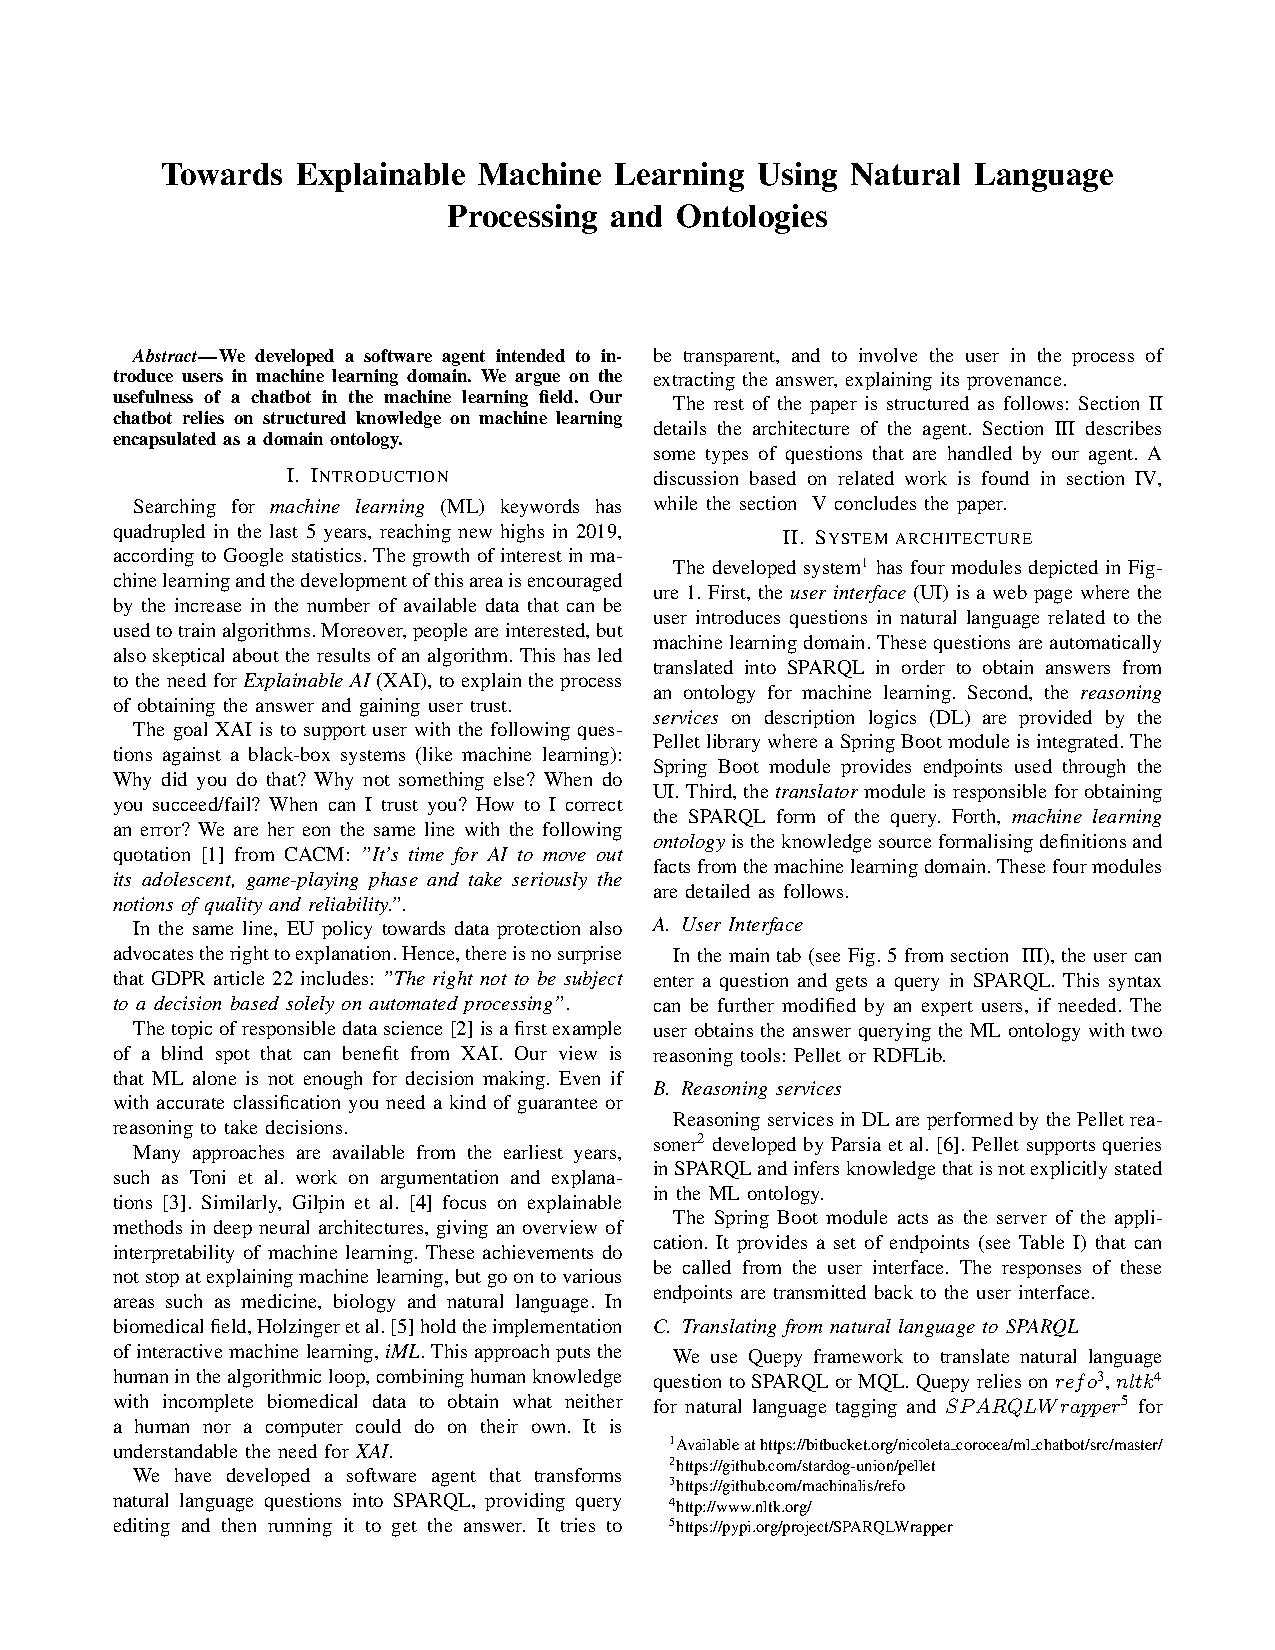
\includepdf[pages=-,pagecommand={},width=\textwidth]{articol_extins.pdf}



\end{document}
